%%%%%%%%%%%%%%%%%%%%%%%%%%%%%%%%%%%%%%%%%%%%%%%%%%%%%%%%%%%%%%%%%%%%%%%%%%%
%
% Trabajo de fin de máster v1.0
% Guillermo Sánchez Brizuela
%
%%%%%%%%%%%%%%%%%%%%%%%%%%%%%%%%%%%%%%%%%%%%%%%%%%%%%%%%%%%%%%%%%%%%%%%%%%%

% Qué tipo de documento estamos por comenzar:
\documentclass[a4paper, 11pt]{article}
% Esto es para que el LaTeX sepa que el texto está en español:
\usepackage[spanish,es-tabla]{babel}
\selectlanguage{spanish}
% Esto es para poder escribir acentos directamente:
\usepackage[utf8]{inputenc}
\usepackage[T1]{fontenc}
% Para texto tachado
\usepackage[normalem]{ulem}
% Imágenes en el lateral
\usepackage{wrapfig}
% Tablas
\usepackage{booktabs}
% Anexos
\usepackage{appendix}
%Tablas
\usepackage{float}
\usepackage{tabularx}
%\usepackage{subcaption}
% Leyendas
\usepackage{caption}
\captionsetup{justification=centering}
% Bibliografia en la tabla de contenidos
\usepackage[nottoc,notlot,notlof]{tocbibind}
% Tablas
\usepackage{booktabs}
\usepackage[table,xcdraw]{xcolor}

%\setlength{\parskip}{\baselineskip}
\edef\restoreparindent{\parindent=\the\parindent\relax}
\usepackage{parskip}
\restoreparindent

% Definición de un nuevo comando
\newcommand{\textbfit}[1]{\textbf{\textit{#1}}}



%% Asigna un tamaño a la hoja y los márgenes
\usepackage[a4paper,top=3cm,bottom=2cm,left=2.5cm,right=2.5cm,marginparwidth=2cm]{geometry}

%% Paquetes de la AMS
\usepackage{amsmath, amsthm, amsfonts}
%% Para añadir archivos con extensión pdf, jpg, png or tif
\usepackage{graphicx}
\usepackage[colorinlistoftodos]{todonotes}
\usepackage[colorlinks=true, allcolors=blue]{hyperref}
%% Simbolo de grado
\usepackage{gensymb}
%% Imágenes en vertical
\usepackage{subfig}
\usepackage{graphicx}
%% Algoritmos y pseudocódigo
\usepackage{algorithm}
\usepackage[noend]{algpseudocode}

\usepackage{nomencl}
\makenomenclature
\nomenclature{Estática}{(Imagen) Capturada o generada de forma individual y no como parte de un vídeo.}
\nomenclature{Vídeo}{Sucesión de imágenes continua que aporta ilusión de movimiento.}
\nomenclature{Online}{(Procesamiento) Que ocurre a medida que llega nueva información.}
\nomenclature{Offline}{(Procesamiento) Que trabaja sobre información previamente recogida.}
\def\nomname{Terminología}

%% Primero escribimos el título
\title{Borrador TFM/Memoria de prácticas: Estimación de Profundidad Monocular Online con Transformers Eficientes}
\author{Guillermo Sánchez Brizuela\\
  \small Universidad de Valladolid\\
  \small Valladolid, España
  \date{}
}

%% Después del "preámbulo", podemos empezar el documento

\begin{document}

\begin{titlepage}
\centering
\begin{figure}[t]
	\centering
	
\includegraphics[scale=0.35]{imagenes/gsi.png}
    \vspace{0.5cm}
\end{figure}%
	{\LARGE Memoria del trabajo realizado durante la estancia en el Grupo de Sistemas Inteligentes\par}
	\vspace{3cm}
	{\huge\bfseries Estimación de Profundidad Monocular Online con Transformers Eficientes\par}
	\vspace{0.5cm}
    {\LARGE Contexto y estado del arte\par}
    \vspace{3cm}
	{\Large\itshape Guillermo Sánchez Brizuela\par}
	\vspace{0.5cm}
	{\Large Universidad de Valladolid, curso 2020-2021\par}
	\vfill
\end{titlepage}

%% Imprimimos la nomenclatura
% \todo[inline]{Repasar las definiciones.}
% \printnomenclature[3cm]

%% Tabla de contenidos
{
    \setcounter{tocdepth}{4}
    \setcounter{secnumdepth}{4}
    \hypersetup{linkcolor=black}
    \tableofcontents
}

\newpage

%% Hay que decirle que incluya el título en el documento
% \maketitle

%% Aquí podemos añadir un resumen del trabajo (o del artículo en su caso) 
% \begin{abstract}
% Lorem ipsum.
% \end{abstract}

% \todo[inline]{Hacer portada y buscar normas del tfm. (TFM)}
%% Iniciamos "secciones" que servirán como subtítulos
\section{Introducción}

Cuando usamos una cámara para capturar una imagen o un vídeo, creamos una representación bidimensional de lo que es en realidad una escena tridimensional. Para conseguir esta reducción de dimensiones, se proyectan en un plano, cada uno de los puntos visibles. Al realizar esta proyección, se pierde una gran cantidad de información relacionada con la profundidad. Esto es debido a que los puntos ahora representados en el plano bidimensional podían encontrarse a cualquier distancia siempre y cuando estuviesen situados en la recta que atraviesa el punto verdadero y el centro de la cámara (Figura \ref{fig:proyeccion-perspectiva}). Es decir, existen infinitas escenas tridimensionales con la misma proyección perspectiva.

% TODO: Repasar los finales de línea de esta imagen
\begin{figure}[H]
\centering
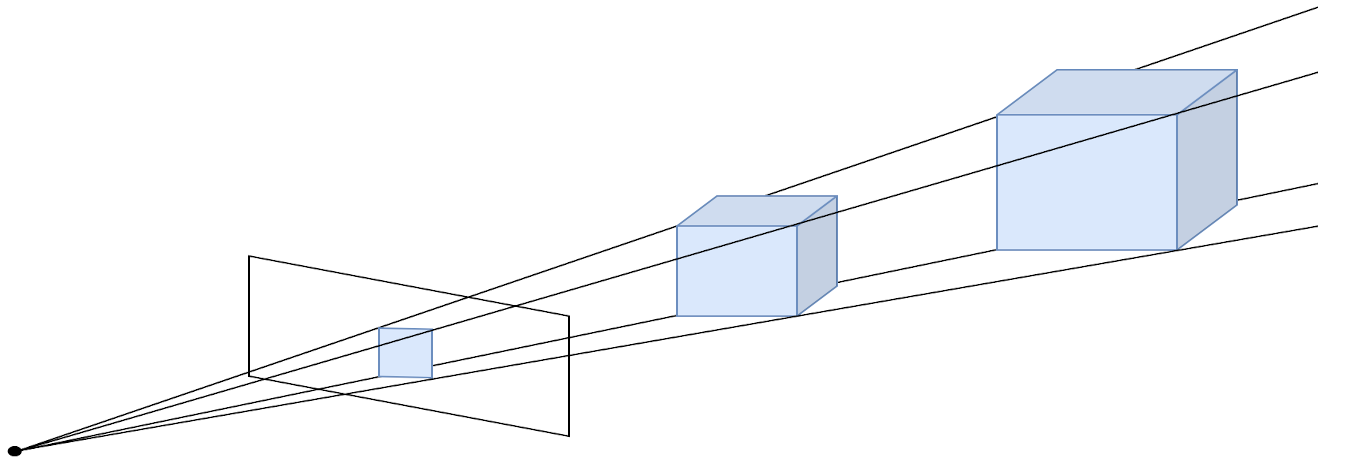
\includegraphics[width=0.65\linewidth]{imagenes/proyeccion-perspectiva.png} 
\captionsetup{width=.8\linewidth}
\caption{Proyección perspectiva y ambigüedad de escala.}
\label{fig:proyeccion-perspectiva}
\end{figure}

Existen soluciones \textit{hardware} capaces de capturar escenas tridimensionales sin esta perdida de información, por ejemplo: sensores LiDAR, cámaras de tiempo de vuelo, o conjuntos de cámaras para llevar a cabo estereovisión\footnote{Con una pareja de cámaras de posiciones conocidas, es posible estimar la profundidad a partir de la disparidad geométrica entre las dos imágenes capturadas.}\cite{hartley_zisserman_2004}. Sin embargo, estas soluciones requieren de sensores adicionales, con el incremento de material, coste y peso que esto conlleva. Es por esto por lo que recuperar la profundidad (o una estimación de esta) a partir de una imagen obtenida con una cámara corriente sería de gran utilidad, por ejemplo:

\begin{itemize}
    \item En diferentes tareas dentro de múltiples campos de aplicación: Navegación robótica y conducción autónoma, empleando la profundidad para reconstruir mapas o calcular el cambio en la posición del agente (odometría visual, VSLAM); detección de superficies y capacidad de incluir oclusión en aplicaciones de realidad aumentada; generación de modelos 3D a través de fotografías (fotogrametría); efectos fotográficos en aplicaciones móviles (efecto \textit{Bokeh}); etc.
    \item Como información adicional o etapa intermedia en otras tareas típicas en visión artificial: detección de objetos, segmentación, clasificación, etc.
\end{itemize}

% https://www.ncbi.nlm.nih.gov/books/NBK11512/
Si observamos, nunca mejor dicho, el sistema visual de los humanos, podemos comprobar como este es un sistema estereoscópico compuesto por dos  ``cámaras''  (los ojos) y un cerebro que interpreta la disparidad entre estas imágenes para obtener una estimación de la profundidad a la que se encuentra cada objeto que vemos. No obstante, si nos tapamos un ojo, aunque con peores resultados, somos capaces de estimar la distancia a la que se encuentran los elementos que están dentro de nuestro campo visual, manteniendo, en una gran mayoría de las ocasiones, la capacidad de distinguir cuáles están más cerca y cuáles más lejos. Esto se debe en gran parte a una serie de sesgos cognitivos que los humanos hemos aprendido a medida que crecemos, conocidos como pistas monoculares (pueden ser dinámicas o estáticas, en función de si consideran la información a lo largo del tiempo, por ejemplo, objetos en movimiento), y que no solo se emplean cuando nos tapamos un ojo, si no que también los emplea el cerebro cuando vemos con los dos ojos. Algunas de las principales pistas monoculares (estáticas) \cite{Kalloniatis2005-pc} son: el tamaño relativo con el que observamos un objeto en función de la distancia a la que se encuentre; la oclusión de los elementos que están más próximos que otros; la convergencia de líneas paralelas a medida que se alejan, por ejemplo, en carreteras o vías; el cambio en el tono del color de los objetos lejanos debido a la dispersión de la luz; o la forma de los reflejos y las sombras que producen los elementos, originados por las fuentes de luz de la escena.

No obstante, realizar este análisis de las imágenes monoculares que tan eficientemente llevamos a cabo los humanos en un ordenador de forma automática empleando técnicas de visión artificial tradicional roza lo imposible. 

Las limitaciones de este tipo de técnicas no solo aparecen en la estimación de profundidades, si no que están presentes en una gran parte de las tareas propias de la visión artificial. Buscando dejar atrás estas limitaciones, en los últimos años se han desarrollado un gran número de sistemas de aprendizaje automático profundo diseñados para trabajar con imágenes. Estos sistemas, pese a tener ciertos inconvenientes, han conseguido ofrecer unos muy buenos resultados junto a una mucho mayor robustez y capacidad de generalización ante modificaciones en las entradas (cambios de entorno, color, luz, orientación de los elementos, etc.), muy frecuentes en los entornos reales no controlados.

Dentro de estas técnicas, en general, y especialmente para la estimación de profundidades, las redes neuronales convolucionales han prevalecido como las arquitecturas que mejores resultados aportaban. No obstante, en los últimos años han surgido otro tipo de arquitecturas, los \textit{transformers} \cite{NIPS2017_3f5ee243}, que presentan resultados muy competitivos. En vista de esto, este trabajo revisa el estado del arte actual en estimación de profundidad monocular y explora una de las arquitecturas que mejores resultados consigue, DPT \cite{visiontransformersDPT}, reproduciendo su entrenamiento y modificándola para disminuir su tamaño y acelerar la inferencia de resultados, es decir, reducir el tiempo necesario para estimar la profundidad en una imagen dada. 

\subsection{Motivación}

Este trabajo tiene dos motivaciones claramente diferenciadas, la primera, académica y la segunda más aplicada. En primer lugar, para poder trabajar en el campo de la estimación de profundidades, es necesario explorar y conocer las distintas técnicas que han surgido a lo largo de los años, tanto las bases y los primeros enfoques para resolver el problema, como las soluciones especializadas que conforman el estado del arte. Por lo tanto, en este trabajo se pretende resumir y agrupar las principales técnicas para poder, posteriormente, revisar y estudiar los temas que se tratan de una manera dirigida y ordenada.

Por otro lado, los modelos del estado del arte tienden a ser (con excepciones) cada vez más complejos, tienen un mayor número de parámetros, y precisan de grandes cantidades de datos para ser entrenados. Esto conlleva una perdida de accesibilidad al desarrollo y experimentación con dichas arquitecturas, que necesitan una infraestructura costosa para ejecutarse. Además, este incremento en tamaño de los modelos hace que sus velocidades de ejecución e inferencia de resultados se vea afectada. En muchas de las aplicaciones mencionadas en el apartado anterior, el tiempo de inferencia es un factor crítico, ya que muchas veces el procesamiento de las imágenes debe llevarse a cabo en entornos con recursos computacionales limitados y de forma \textit{online}, es decir, procesar las imágenes a medida que están disponibles (sin considerar las restricciones de un entorno de tiempo real). En el caso de que la inferencia de los modelos no se lleve a cabo en dispositivos embebidos y recaiga en servidores a los que los clientes hacen peticiones, un mayor tiempo de ejecución se traduce directamente en un incremento de costes, por lo que tampoco es despreciable. Por estas razones, en este trabajo se busca modificar una de los modelos del estado del arte en estimación de profundidades a partir de imágenes monoculares para reducir su tamaño y tiempo de inferencia reduciendo lo mínimo posible la calidad de los resultados.

\subsection{Objetivos}
Los objetivos principales de este Trabajo Fin de Máster, son:
\begin{enumerate}
	\item Llevar a cabo una revisión del estado del arte relacionado con la estimación de profundidades en imágenes monoculares. Más concretamente, en aquellas técnicas que empleen aprendizaje automático, prestando especial atención a las arquitecturas basadas en \textit{transformers} y sus variantes eficientes.
    \item Estudiar una arquitectura del estado del arte de estimación de profundidades y modificar su estructura para acelerar la inferencia hasta obtener modelos capaces de procesar imágenes de forma \textit{online}. Además, una vez definidos los modelos con las variaciones planteadas, comparar sus resultados tras ajustarles a un \textit{dataset} concreto.
    \item Explorar diferentes técnicas generales para acelerar el entrenamiento e inferencia de los modelos de aprendizaje automático profundo. \todo{Checkear esto}
    \item Diseñar una solución en la nube que permita desplegar de forma automática instancias que ejecuten los experimentos necesarios, es decir, entrenando los distintos modelos planteados.
\end{enumerate}


\subsection{Estructura del documento}
Este trabajo Fin de Máster está organizado de la siguiente manera: Primero, se han expuesto en esta sección de Introducción tanto la motivación detrás del proyecto como los objetivos que se plantearon al comenzarlo; a continuación, en el segundo capítulo se contextualiza el trabajo repasando las bases teóricas sobre las que se apoya su desarrollo, revisando también el Estado del Arte de estos campos; en el tercer capítulo, se presentan y justifican tanto los materiales empleados para el desarrollo del trabajo como la metodología que se ha seguido; después, en el cuarto capítulo, se definen y explican aquellos desarrollos especialmente significativos dentro del trabajo para continuar en el quinto capítulo con los resultados que se han obtenido, haciendo especial hincapié en la influencia en estos resultados de cada uno de los desarrollos llevados a cabo. Por último, se incluye en el capítulo seis una discusión de los resultados y en el capítulo siete las conclusiones del documento junto a una serie de líneas de investigación futuras que podrían explorarse para continuar trabajando en el contexto de este proyecto. 

\todo[inline]{Poner algo de los anexos?}

\clearpage

\section{Marco teórico y Estado del Arte}

\subsection{Inteligencia Artificial, Aprendizaje automático, y Aprendizaje Profundo}
La Inteligencia Artificial (IA), engloba el estudio de agentes que perciben un entorno y actúan en consecuencia. Este campo, comprende multitud de disciplinas y técnicas aplicables en incontables escenarios. Dentro de los subcampos que conforman la IA están por ejemplo los sistemas expertos, los modelos probabilísticos, la lógica difusa, o, de especial importancia en este trabajo, el aprendizaje automático (\textit{Machine Learning} - \textit{ML}). 

El aprendizaje automático estudia diferentes modelos que son capaces de extraer información de forma automática a partir de un conjunto de datos. En función de qué información tengan estos datos y qué se busque hacer con ella, es posible distinguir entre aprendizaje supervisado (donde los datos están etiquetados con lo que se quiere aprender), aprendizaje no supervisado (donde los datos no tienen anotaciones y se busca encontrar relaciones o extraer información sobre ellos), aprendizaje semisupervisado (si se usan datos etiquetados y no etiquetados) o aprendizaje por refuerzo (si se emplea una función de recompensa y se deja al modelo elegir las acciones que lleva a cabo).

Más centrado aún en el proyecto está el aprendizaje profundo (\textit{Deep Learning} - \textit{DL}), un subcampo del aprendizaje automático donde se emplean modelos y técnicas con una complejidad computacional mayor que, en consecuencia, requieren de una cantidad de datos acorde para poder aprender satisfactoriamente.

Cabe mencionar que pese a que muchos de los conceptos explicados a continuación son perfectamente validos en otras modalidades, este trabajo se centra en el aprendizaje profundo supervisado y por lo tanto el marco teórico se ajusta y limita a este. 

\subsection{Redes neuronales}
Las redes neuronales (en inglés, \textit{Neural Networks} - NN), son sistemas computacionales inspirados en una versión simplificada de las neuronas biológicas. Estas neuronas artificiales, están definidas por una serie de elementos: entradas, \textbf{pesos}, \textbf{bias}, \textbf{función de activación} y salida. El valor que toma la salida, siguiendo la notación de la Figura \ref{fig:neurona}, viene dado por la ecuación $y = f(Wx + b)$.

\begin{figure}[H]
\centering
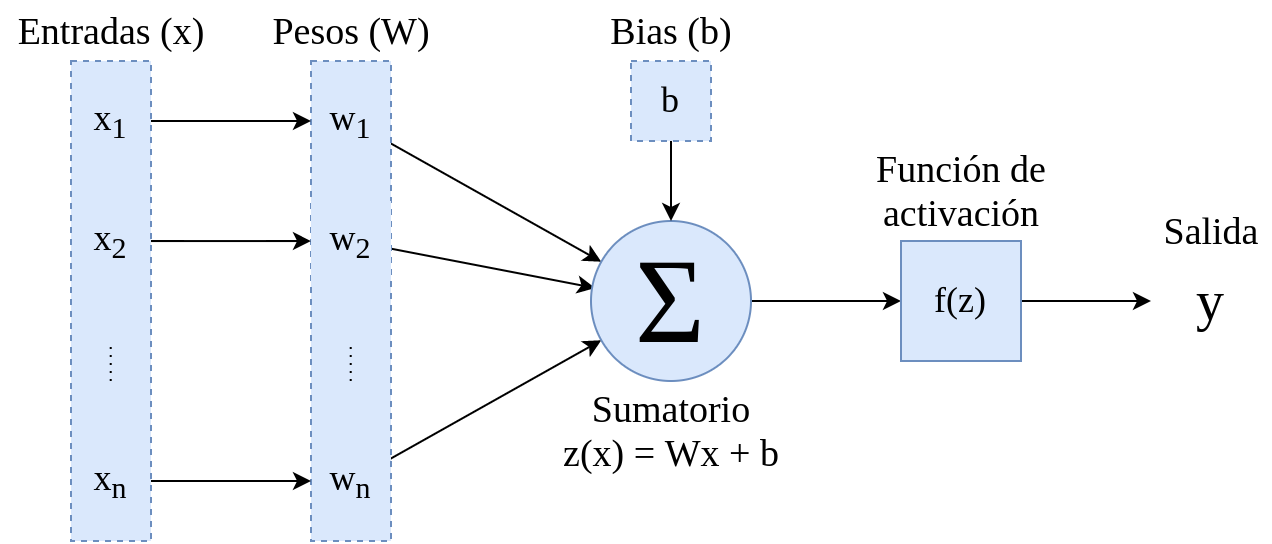
\includegraphics[width=.75\linewidth]{imagenes/neurona.png} 
\captionsetup{width=.5\linewidth}
\caption{Estructura de una neurona artificial.}
\label{fig:neurona}
\end{figure}

Uno de los puntos más importantes de las NN, es que con un conjunto de neuronas lo suficientemente grande y funciones de activación no lineales, las NN pueden aproximar cualquier función continua (\textit{Universal approximation theorem} \cite{}). Por desgracia, ajustar los parámetros (pesos y bias) de cada una de las neuronas de dicha red para aproximar la función deseada no es un problema trivial. 

Una de las soluciones más comunes, es, de forma iterativa, modificar los parámetros de forma que minimicen la distancia entre la salida de la red y la función que se busca aproximar. Para esto, se emplea la propagación hacia atrás (\textbfit{backpropagation}) \cite{}, que necesita: un \textbf{optimizador} (en los que se profundiza en la sección TODO), un \textbf{conjunto de entradas con salidas conocidas} y una \textbf{función de perdida} que se emplea como aproximación optimizable de la distancia previamente mencionada. Este algoritmo, de forma simplificada, consiste en:

\begin{enumerate}
\item Calcular la salida de la red a partir de las entradas de las cuales conocemos la salida esperada (\textbfit{forward pass}).
\item Emplear una \textbf{función de pérdida} para calcular una medida del error entre la salida obtenida y la salida esperada.
\item Calcular las derivadas parciales del error respecto de cada uno de los parámetros (\textbf{pesos} y \textbfit{bias}) que se quieren ajustar.
\item Ajustar los valores de los parámetros en función de su influencia en el error empleando un optimizador concreto.
\end{enumerate}

Estos pasos, normalmente se repiten varias veces para cada ejemplo disponible (entendiendo como ejemplo las parejas entrada-salida conocida). En el contexto de las redes neuronales, este proceso de ajuste se conoce como \textbf{entrenamiento} y cada una de las iteraciones que la red realiza sobre el conjunto de ejemplos se conoce como época (\textit{epoch}, en inglés). 

El proceso de entrenamiento, sin embargo, hay que controlarlo y validarlo de alguna forma, ya que existe el riesgo de sobreajustar los parámetros de la red neuronal a los datos de entrenamiento, siendo el modelo incapaz de generalizar a datos no antes vistos, este sobreajuste se conoce en inglés como \textbfit{overfitting}. Para controlar si el modelo se está sobreajustando, es común dividir el conjunto de datos en tres subconjuntos: entrenamiento, validación, y evaluación. El conjunto de entrenamiento, se emplea para ajustar los parámetros del modelo; el de evaluación, para comprobar si hay \textit{overfitting} y para elegir entre distintas configuraciones de un mismo modelo o distintos modelos; y el de evaluación, para calcular las métricas finales del modelo elegido para un problema concreto. En el trabajo de ... \cite{El paper ese de 50 páginas con splits} se presentan distintas formas de hacer estas particiones, en este trabajo, no obstante, se emplearán particiones establecidas en la literatura para los conjuntos de datos empleados (Ver sección TODO).

%TODO ? sesgo/varianza

En esta introducción, se han mencionado algunos conceptos en los que se profundiza a continuación prestando especial atención a los elementos que aparecen en este trabajo.

\subsubsection{Funciones de activación}
Tal y como se puede ver en la Ecuación \ref{}, la función de activación transforma la suma del \textit{bias} y el producto de los pesos y las entradas para obtener el valor de salida. En la Figura \ref{fig:funciones-activacion}, es posible observar varias de estas funciones junto con sus ecuaciones.

\begin{figure}[H]
\centering
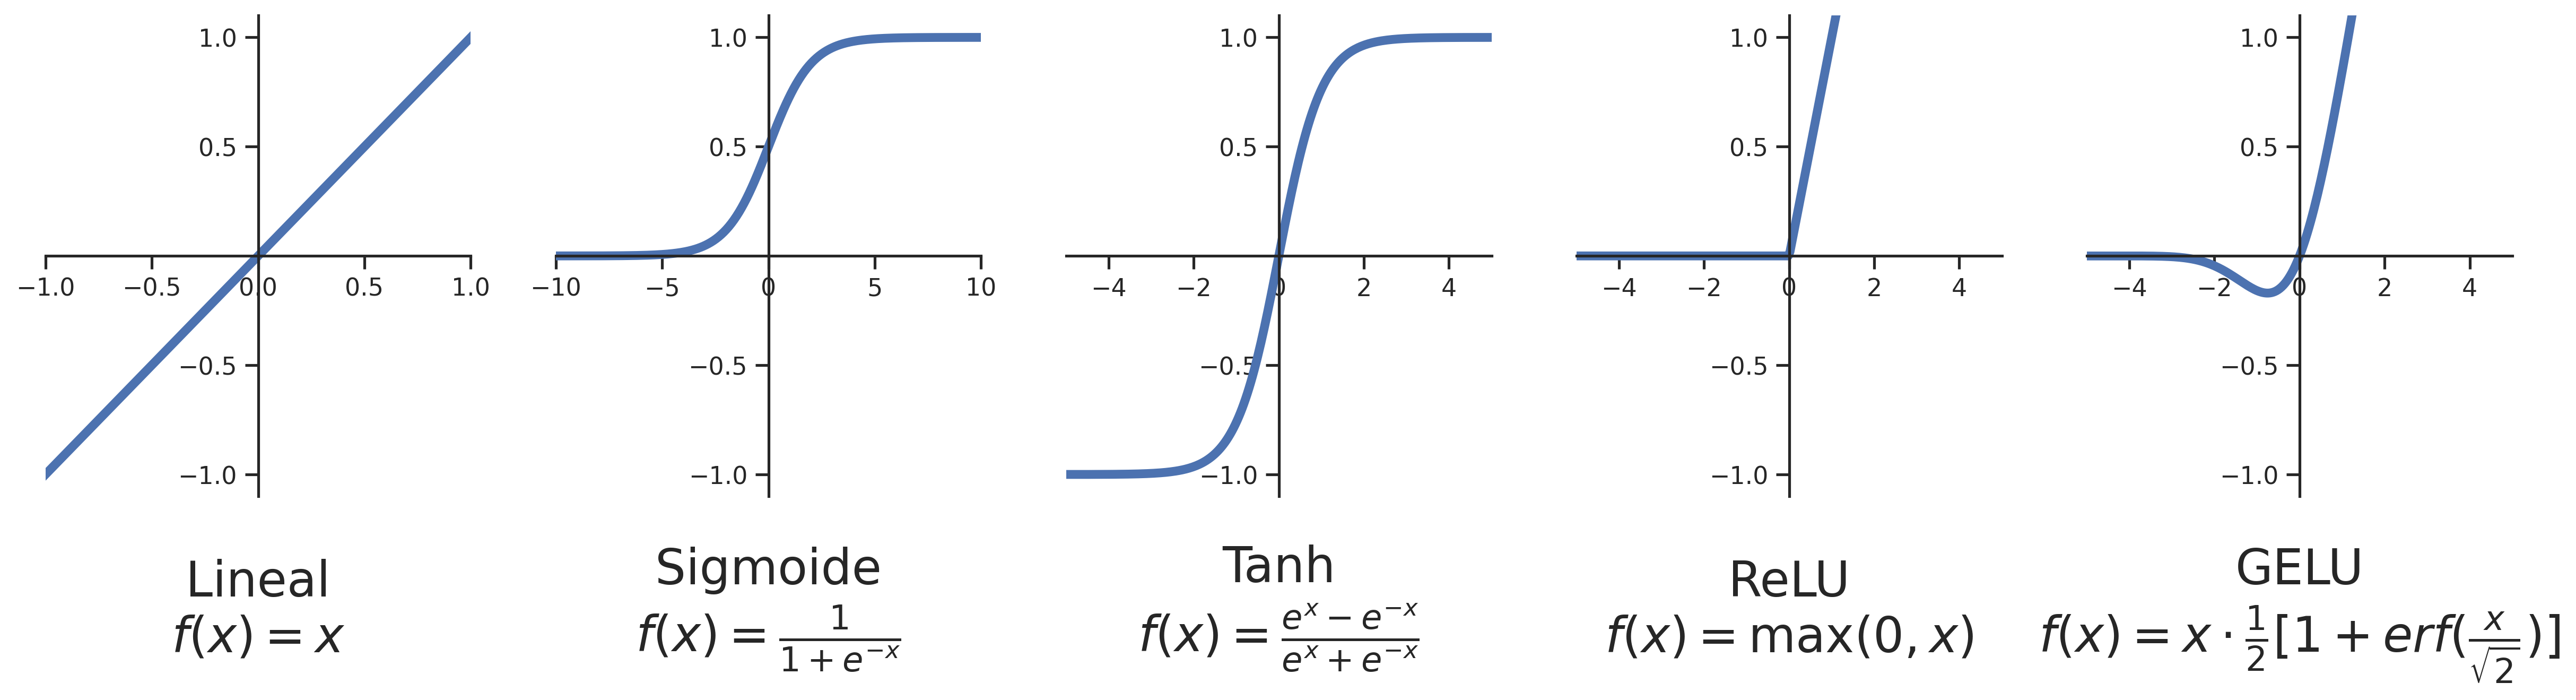
\includegraphics[width=\linewidth]{imagenes/funciones_activacion.png} 
\captionsetup{width=.8\linewidth}
\caption{Funciones de activación.}
\label{fig:funciones-activacion}
\end{figure}

La primera de estas funciones de activación es la función de activación lineal. Esta función, no suele emplearse, ya que si concatenamos múltiples neuronas con activaciones lineales, serían equivalentes a una sola neurona con la función lineal equivalente. Por esta razón, son funciones no lineales como la sigmoide, la tangente hiperbólica, ReLU (\textit{Rectified Linear Unit}) \ref{} o GELU \cite{} (\textit{Gaussian Error Linear Unit}) las que suelen aparecer en las arquitecturas más populares. 

Cada una de estas funciones de activación tiene características propias que las hacen diferentes entre si. La tangente hiperbólica, aún siendo similar a la sigmoide, es simétrica y tiene unos gradientes más fuertes en las zonas cercanas al cero, lo que origina que sus salidas sean valores pequeños centrados en cero y que el entrenamiento sea más rápido \cite{paper-lecun-efficient-backprop}. La función ReLU, por otro lado, pese a ser parcialmente lineal, puede aproximar funciones no lineales gracias a su definición a trozos, además, el gradiente para los valores positivos es constante $(1)$, reduciendo en gran medida el desvanecimiento de los gradientes cuando se definen redes neuronales con un gran número de capas. Por último, la función GELU, es comúnmente empleada en las arquitecturas basadas en \textit{transformers} (Ver sección TODO) y mantiene el gradiente constante en valores positivos a la vez que añade una ligera ponderación a los valores negativos cercanos al cero.

\subsubsection{Funciones de pérdida}
Las funciones de pérdida, tal y como se ha mencionado previamente, son aproximaciones optimizables de la distancia o error entre el valor real a predecir y la predicción realizada. Dentro de estas funciones, cuyo valor se busca minimizar, existen diferentes situaciones que pueden dificultar el aprendizaje de los modelos, por ejemplo, los mínimos locales, donde los valores de la función de pérdida son menores que los valores de su entorno, originando que los gradientes se desvanezcan y detengan el proceso de optimización, o los puntos de silla (\textit{saddle points}), donde, pese a no haber un mínimo local, los gradientes también se desvanecen deteniendo la minimización.

\subsubsection{Optimizadores}
Los optimizadores son algoritmos que minimizan el valor de la función de pérdida ($f(\theta)$) ajustando los parámetros ($\theta$) de los modelos, entre otras cosas, en base a la influencia de estos parámetros en el error obtenido en dicha función. Esta influencia se obtiene calculando las derivadas parciales del error respecto de cada parámetro (gradiente: $\nabla_{\theta} f_t(\theta_{t-1})$), y, en función del algoritmo que se elija, puede verse afectada por distintos factores. Algunos de los optimizadores más empleados son SGD \cite{}, AdaGrad \cite{}, RMSProp \cite{}, Adam \cite{} o Adamw \cite{}.

El descenso de gradiente tradicional promedia los gradientes del error en todos los ejemplos disponibles para actualizar los parámetros. La modificación que introduce el \textbf{SGD (\textit{Stochastic Gradient Descent})}, es actualizar los parámetros tras ver cada uno de los ejemplos. De esta forma, se acelera el entrenamiento ya que aunque cada ajuste no es óptimo, se actualizan mucho más frecuentemente. Además, el ruido intrínseco de cada ejemplo tiene un efecto regularizador que puede ayudar a salir de mínimo locales.

No obstante, gracias a la capacidad de procesamiento paralelo de las tarjetas gráficas es muy común promediar el cálculo del error en pequeños subconjuntos (\textbfit{batch}) de todos los datos disponibles. Esto se conoce como \textit{Mini Batch Gradient Descent} y el tamaño (\textbfit{batch size}) que se elija influye directamente en diferentes factores como son la velocidad de entrenamiento, la rapidez para converger, o el punto al que se converge \cite{on batch size paper}.

Estos tres algoritmos, y en general la mayoría de los optimizadores, controlan el cambio de los parámetros mediante un hiperparámetro conocido como tasa de aprendizaje (\textit{learning rate}: $\gamma$), que se multiplica por el valor del gradiente de la función de pérdida respecto de los parámetros (Ecuación \ref{eqn:sgd}).

\begin{equation}
\label{eqn:sgd}
\theta_t = \theta_{t-1} - \gamma (\nabla_{\theta} f_t(\theta_{t-1}))
\end{equation}

En el caso del \textit{Mini Batch Gradient Descent}, al promediar los gradientes de varios ejemplos se reduce el ruido del SGD. Inspirado por el concepto físico de \textbf{Momento}, es posible añadir a estos optimizadores una modificación para que se consideren también los gradientes de los pasos anteriores del optimizador. De esta forma, se reduce el ruido y se hace más robusta la optimización frente a mínimos locales. El momento se controla con un hiperparámetro $\mu$ siguiendo la Ecuación \ref{eqn:momento}, donde $v_t$ es el Momento en un paso concreto y $g_{t, t-1}$ los gradientes correspondientes a este paso. 

\begin{equation}
\label{eqn:momento}
v_t = \mu v_{t-1} + g_{t, t-1}
\end{equation}

Este cálculo multiplica los momentos anteriores de forma recursiva por un valor menor que uno, de forma que influyen todos los gradientes anteriores, pero cada vez con menos fuerza. Esto se puede ver comprobar matemáticamente desarrollando la Ecuación \ref{eqn:momento} (Ecuación \ref{eqn:momento2}). Finalmente, este momento toma la posición del gradiente en la actualización de los parámetros (Ecuación \ref{eqn:momento3}).

\begin{equation}
\label{eqn:momento2}
v_t = \mu^2 v_{t-2} + \mu g_{t-1, t-2} + g_{t, t-1} = \sum_{i=0}^{t-1}\mu^{i}g_{t-i, t-i-1}
\end{equation}
\begin{equation}
\label{eqn:momento3}
\theta_t = \theta_{t-1} - \gamma (v_t)
\end{equation}

\textbf{AdaGrad (\textit{Adaptative Gradients})}, otro optimizador, también modifica el descenso del gradiente para reducir las tasas de aprendizaje en aquellos parámetros que han tenido mayores derivadas parciales dividiendolas entre la suma de los gradientes ($g$) anteriores (Ecuaciones \ref{eqn:adagrad} y \ref{eqn:adagrad2}). Estos gradientes se acumulan durante toda la optimización, por lo que es especialmente efectivo en datos dispersos donde no en todos los ejemplos se dispone de todas las características, donde las características que no se hayan visto tan frecuentemente tendrán actualizaciones mayores. Esto, sin embargo, también ralentiza el algoritmo, ya que según avanza el proceso, las actualizaciones de los parámetros son menores, llegando incluso a impedir que se alcance a un mínimo aceptable.

\begin{equation}
\label{eqn:adagrad}
acumulaci\acute{o}n_t = acumulaci\acute{o}n_{t-1} + g^{2}_{t}
\end{equation}
\begin{equation}
\label{eqn:adagrad2}
\theta_t = \theta_{t-1} - \gamma \frac{g_t}{\sqrt{acumulaci\acute{o}n_t}}
\end{equation}

% https://towardsdatascience.com/a-visual-explanation-of-gradient-descent-methods-momentum-adagrad-rmsprop-adam-f898b102325c

\textbf{RMSProp (\textit{Root Mean Square Propagation})} soluciona el problema de la velocidad de AdaGrad añadiendo un factor de decaimiento. Este factor de decaimiento (\textit{decay rate}: $\alpha$), escala de forma recursiva la suma acumulada de los gradientes anteriores (media movil exponencialmente ponderada - \textit{Exponential weighted moving averages}), por lo que a medida que el optimizador avanza, la influencia de los gradientes anteriores disminuye. De esta forma, se mantienen los beneficios de AdaGrad evitando reducir indefinidamente la magnitud de la actualización de los parámetros (Ecuaciones \ref{eqn:RMSProp} y \ref{eqn:RMSProp2}).

\begin{equation}
\label{eqn:RMSProp}
acumulaci\acute{o}n_t = (\alpha) acumulaci\acute{o}n_{t-1} + (1-\alpha) g^{2}_{t}
\end{equation}
\begin{equation}
\label{eqn:RMSProp2}
\theta_t = \theta_{t-1} - \gamma \frac{g_t}{\sqrt{acumulaci\acute{o}n_t}}
\end{equation}

Por último, \textbf{Adam} y \textbf{AdamW} son dos optimizadores que fusionan las ideas y ventajas detrás del momento y de RMSProp. Para conseguir esto, se vuelve a aplicar la media móvil exponencialmente ponderada, esta vez tanto para el primer como el segundo momento, controlado por dos parámetros $\beta$ (Ecuaciones \ref{eqn:Adam} y \ref{eqn:Adam2}).

\begin{equation}
\label{eqn:Adam}
m_t = \beta_1 m_{t-1} + (1-\beta_1) g_{t}
\end{equation}
\begin{equation}
\label{eqn:Adam2}
v_t = \beta_2 v_{t-1} + (1-\beta_2) g^{2}_{t}
\end{equation}

Además, para reducir la influencia del valor inicial (igual a cero) de $m_0$ y $v_0$, se añade una normalización que sigue las Ecuaciones \ref{eqn:Adam3} y \ref{eqn:Adam4}.

\begin{equation}
\label{eqn:Adam3}
\hat{m}_t = \frac{m_t}{(1-\beta^{t}_{1})}
\end{equation}
\begin{equation}
\label{eqn:Adam4}
\hat{v}_t = \frac{v_t}{(1-\beta^{t}_{2})}
\end{equation}

Una vez calculados estos dos términos, se actualizan los parámetros de forma similar a como se hacía en RMSProp, con la diferencia de que esta vez se multiplica por el momento acumulado y no por los gradientes (Ecuación \ref{eqn:Adam5}).

\begin{equation}
\label{eqn:Adam5}
\theta_t = \theta_{t-1} - \gamma \frac{\hat{m}_t}{\sqrt{\hat{v}_t}}
\end{equation}

En cuanto a la diferencia entre Adam y AdamW, TODO

\subsection{MLP}
El Perceptrón Multicapa, o por sus sigles en ingles, \textbf{MLP} (\textit{Multi Layer Perceptron}), es una de las arquitecturas de red neuronal más básicas y está formado por una capa de entrada, una capa de salida, y un bloque de capas intermedias u ocultas. Estas capas intermedias, son agrupaciones de neuronas donde cada una de las neuronas (normalmente) se conecta con todas las neuronas de la capa anterior y con todas las neuronas de la capa posterior (Figura \ref{fig:mlp}). De esta forma, se crea una sucesión donde las entradas de una neurona son las salidas de las neuronas de la capa anterior y la salida de dicha neurona es una de las entradas de todas las neuronas de la capa siguiente. 

\begin{figure}[H]
\centering
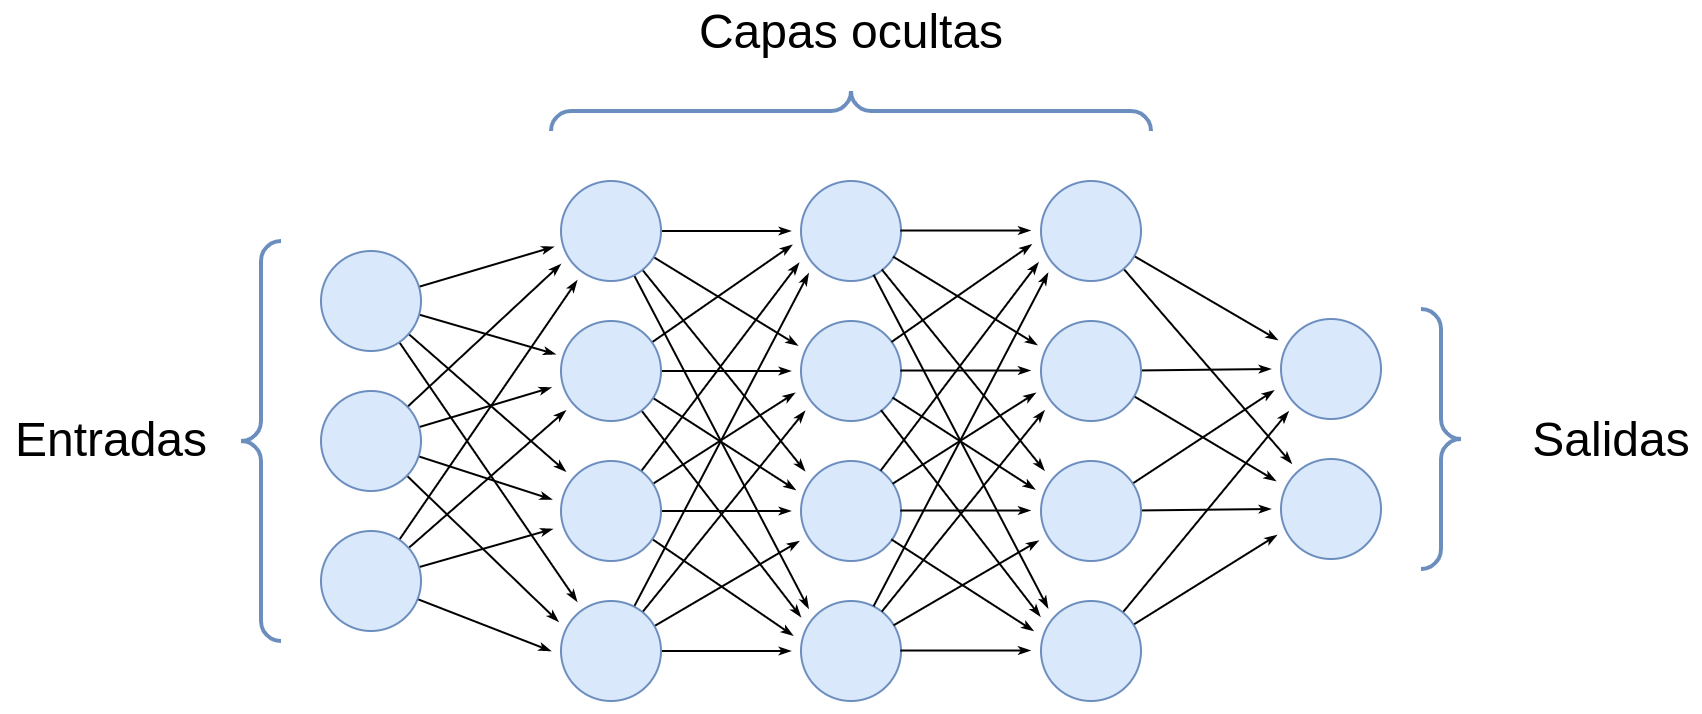
\includegraphics[width=0.8\linewidth]{imagenes/mlp.png} 
\captionsetup{width=.8\linewidth}
\caption{Perceptrón Multicapa.}
\label{fig:mlp}
\end{figure}

\todo[inline]{Este parrafillo no me convence mucho}
Con este tipo de arquitectura, comienza a desdibujarse la linea entre el aprendizaje automático y el aprendizaje profundo, ya que a medida que aumentamos el número de capas intermedias del modelo nos adentramos en el campo del \textit{Deep Learning} y su capacidad de ajuste aumenta.

\subsection{RNN}
Las redes neuronales recurrentes (RNN - \textit{Recurrent Neural Networks}) son un grupo de redes neuronales, introducidas por TODO \cite{rnn}. La arquitectura de estas redes se fundamenta en la utilización repetida de la salida de la propia red en un instante como entrada adicional de la red en el instante siguiente. Para conseguir esto, se mantiene la información en forma de estado escondido (\textit{hidden state}). Gracias a esta transmisión recurrente, es posible transferir información entre entradas sucesivas de la red.

Este tipo de redes está especialmente diseñado para trabajar con entradas secuenciales de valores (series temporales, texto, señales de audio y video, etc.) ya que su arquitectura aprovecha la información de los datos previos y no tiene limitaciones en el tamaño de la secuencia de entrada.

Sin embargo, la ejecución y entrenamiento de este tipo de redes requiere ejecutarlas individualmente con cada uno de los valores de la entrada, haciendo que el proceso sea temporalmente costoso. Además, pese a que se han presentado distintas modificaciones como las celdas GRU (\textit{Gated Recurrent Units}) \cite{gru} o LSTM (\textit{Long Short-Term Memory}) \cite{lstm} que los mitigan, también sufren tanto de desvanecimientos de gradientes por las activaciones sucesivas como de pérdida de información en cadenas de gran tamaño (al codificar toda la información anterior en un estado oculto, llega un punto en el que la información almacenada en instantes alejados temporalmente deja de ser representativa).

\begin{figure}[H]
\centering
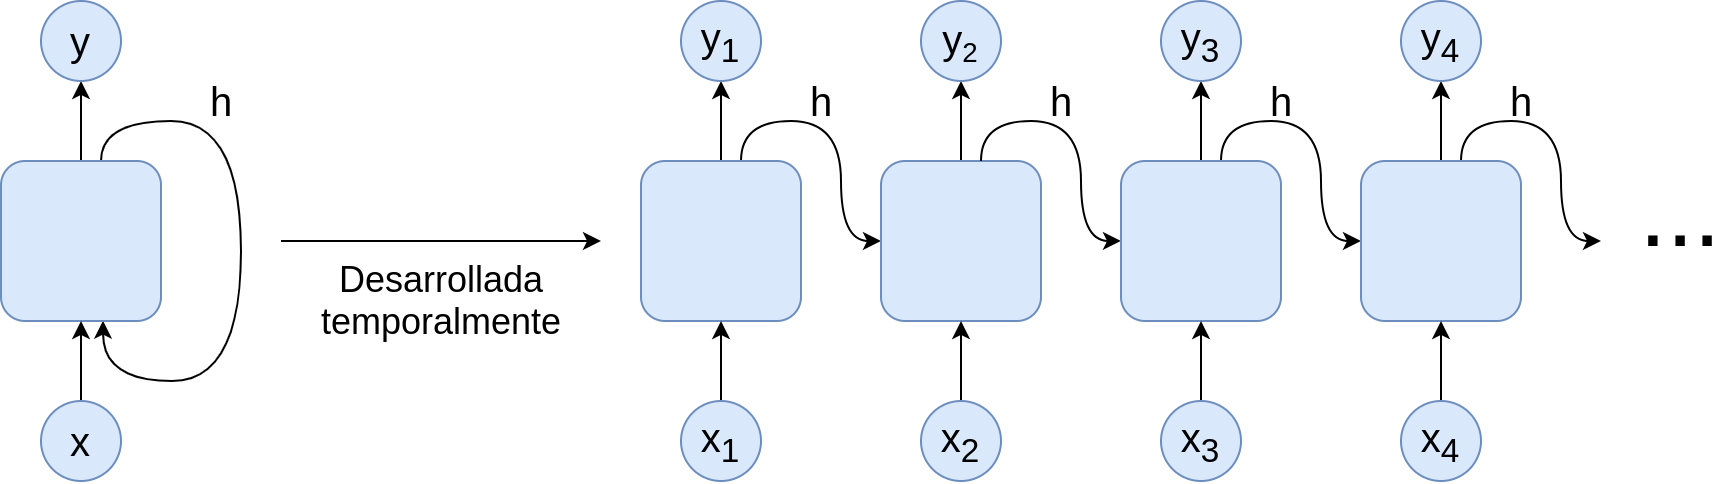
\includegraphics[width=0.8\linewidth]{imagenes/rnn.png} 
\captionsetup{width=.8\linewidth}
\caption{Red recurrente.}
\label{fig:rnn}
\end{figure}

\subsection{CNN}
A la hora de trabajar con imágenes (matrices de dos o tres dimensiones), el número de conexiones, y por lo tanto, parámetros, que tendrían que existir para conectar cada valor de entrada con cada neurona crece enormemente. Las redes convolucionales, no solo lidian con este problema, si no además lo hacen proporcionando muy buenos resultados. Este tipo de redes, se basan en el concepto de núcleo (\textit{kernel}) proveniente del procesamiento digital de imágenes y la operación de convolución, y su origen se atribuye al trabajo de LeCun et al. \cite{}.

Los \textit{kernels} (Figura \ref{fig:convolucion}) son pequeñas matrices (cuyos valores son equivalentes a los pesos vistos anteriormente, y por lo tanto son ajustados durante el entrenamiento) que se convolucionan sobre la imagen de entrada, extrayendo de esta forma mapas de características (también conocidos como mapas de activaciones) que son a su vez la entrada de las siguientes capas convolucionales tras aplicar una función de activación y puede que otras operaciones. En cuanto a la convolución (o correlación cruzada\footnote{La operación matemática de convolución entre dos funciones incluye voltear una de las funciones. Sin embargo, en el campo del Deep Learning, voltear la entrada o el filtro requeriría una operación adicional que solo conllevaría que los pesos obtenidos tras el descenso de gradiente estuvieran también volteados. Por lo tanto, la operación de convolución en redes neuronales realmente es una operación de correlación cruzada donde no se voltea ninguna de las funciones.}), es una operación cuya salida se obtiene desplazando una de las dos matrices y calculando su producto escalar con la otra matriz (Figura \ref{fig:convolucion}). Estas capas, están definidas principalmente por el tamaño del \textit{kernel}, el número de \textit{kernels} que se aplican y la zancada o \textit{stride}, que es el desplazamiento del \textit{kernel} para calcular cada valor de salida y por lo tanto afecta directamente en su tamaño. 

\begin{figure}[H]
\centering
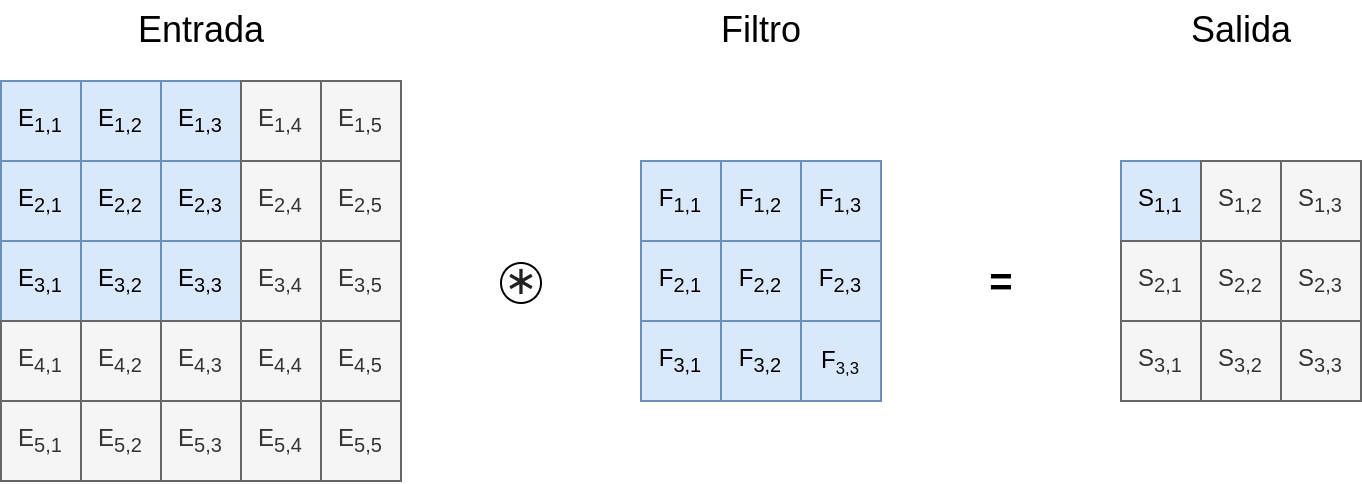
\includegraphics[width=0.8\linewidth]{imagenes/convolucion.png} 
\captionsetup{width=.8\linewidth}
\caption{Operación de convolución con un \textit{kernel} de $3\times3$ y un \textit{stride} de $1$ para uno de los valores de salida.}
\label{fig:convolucion}
\end{figure}

Los \textit{kernels}, normalmente tienden a extraer características de más alto nivel cuanto más adelante están en la red. Esto significa que los mapas de características resultantes en las capas iniciales son características de muy bajo nivel (lineas verticales, horizontales, curvas, esquinas, etc.), mientras que las de las últimas capas extraen características más complejas propias de cada dominio de aplicación \cite{Visualizing and Understanding Convolutional Networks}.

En las redes convolucionales, es común encontrar otras operaciones como son:
\begin{itemize}
\item Pooling: Las capas de \textit{Pooling} se emplean principalmente para reducir el tamaño de los mapas de características resultantes de las capas convolucionales. Para conseguirlo, agrupan un conjunto de valores en un solo valor aplicando una función que normalmente es el máximo (\textit{MaxPooling} - se escoge el máximo valor) o la media (\textit{AveragePooling} - se calcula la media de los valores). La operación de \textit{Pooling} está definida principalmente por dos valores similares a los de la convolución: el tamaño del \textit{kernel}, que define el tamaño del subconjunto de valores; y la zancada o \textit{stride}, que define el número de valores que se traslada el \textit{kernel} cada paso. En la Figura \ref{fig:pooling}, se puede observar una operación de \textit{Pooling} con un \textit{kernel} y un \textit{stride} de $2\times2$ donde cada uno de los valores de la salida se calcula a partir de los valores de la entrada con el mismo color.

\begin{figure}[H]
\centering
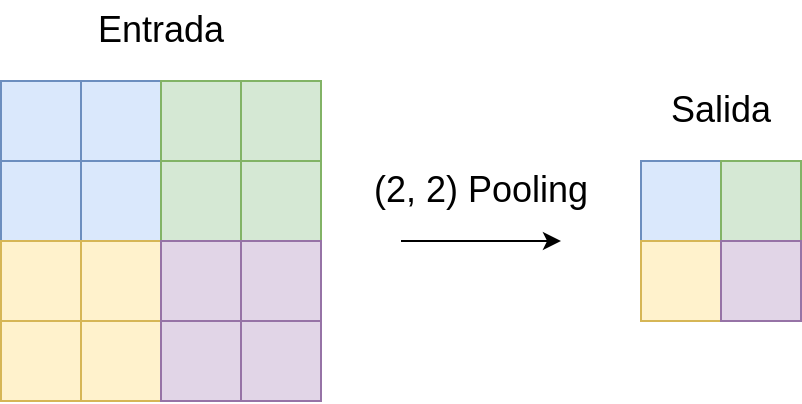
\includegraphics[width=0.5\linewidth]{imagenes/pooling.png} 
\captionsetup{width=.5\linewidth}
\caption{Operación de Pooling2D.}
\label{fig:pooling}
\end{figure}

\item Deconvolución / Convolución transpuesta: TODO
\end{itemize}

\pagebreak

\subsubsection{Conexiones residuales y ResNets}

En el artículo publicado por He et al. \cite{resnet} se presentan las conexiones residuales y la familia de redes ResNet, compuesta por distintos modelos en función de su número de capas. En el momento en el que se publicó dicho estudio, gracias a las conexiones residuales, se consiguió aumentar el número de capas en los modelos del estado del arte en cerca de un orden de magnitud (de las 22 capas de GoogleLeNet \cite{googlelenet} a las 152 capas de ResNet152). Para conseguir esto, las ResNet se apoyan en las conexiones residuales (Figura \ref{fig:residual}), que permiten aumentar tanto la capacidad de aprendizaje de las redes como la calidad de sus resultados.

%\begin{figure}[H]
%\centering
%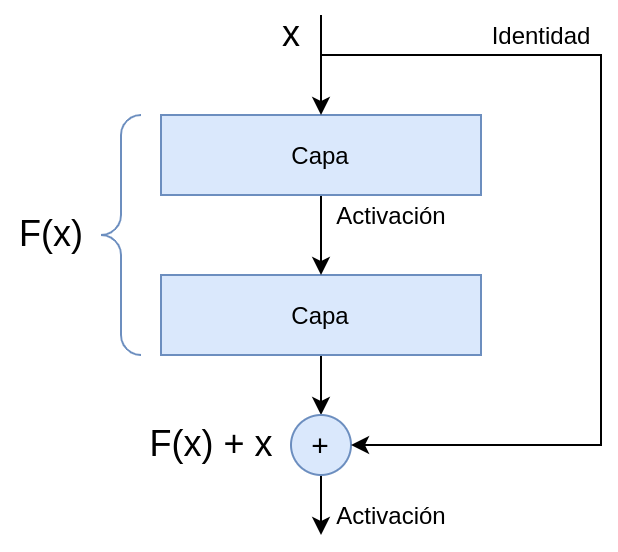
\includegraphics[width=0.5\linewidth]{imagenes/residual-connection.png} 
%\captionsetup{width=.5\linewidth}
%\caption{Conexión residual básica.}
%\label{fig:residual}
%\end{figure}

\begin{wrapfigure}{r}{0.4\textwidth}
\vspace{-10pt}
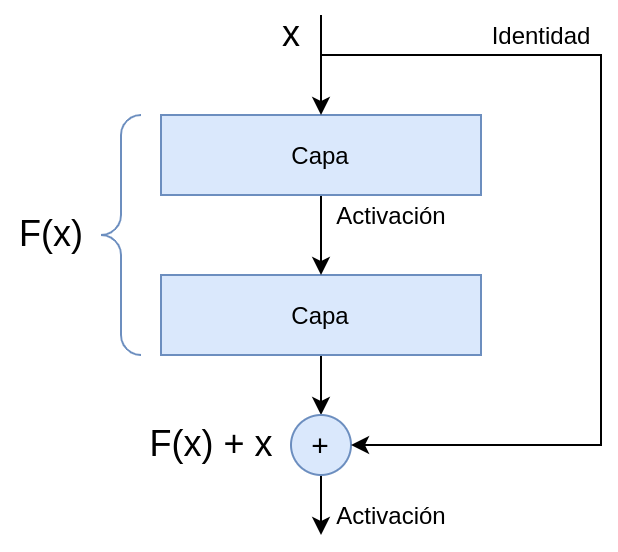
\includegraphics[width=0.95\linewidth]{imagenes/residual-connection.png} 
\caption{Conexión residual básica.}
\label{fig:residual}
\end{wrapfigure}

Las conexiones residuales están motivadas por la idea de que dada una red con una profundidad óptima para una tarea, en teoría, por muchas capas que se incluyesen, el descenso del gradiente sería capaz de hacer que las capas adicionales convergiesen en una función identidad y no perjudicasen los resultados. No obstante, empíricamente se ha comprobado que con las redes neuronales llega un punto en el que añadir más profundidad hace que los resultados empeoren. Aquí es donde entran las conexiones residuales, ya que al pasar hacia adelante la entrada de un bloque de capas y sumarlo a su salida (Figura \ref{fig:residual}), se facilita que el descenso del gradiente reste importancia a la señal que ha atravesado dicho bloque ($F(x)$) en caso de que no mejore a la salida final de la red.

Además, para reducir el uso de recursos computacionales al incrementar el número de capas, las ResNet utilizan conexiones residuales con cuellos de botella (\textit{bottleneck}) para reducir el tiempo de ejecución. Este sistema, en vez de usar como $F(x)$ (Figura \ref{fig:residual}) dos capas convolucionales, emplea tres, siendo la primera y la tercera convoluciones de filtros $1\times1$ (Sección TODO) que se encargan de reducir el número de canales y posteriormente incrementarlo para que se pueda sumar con la entrada. De esta forma, se reducen en gran medida el número de operaciones a realizar en la capa convolucional central, con filtros de tamaño $3\times3$. 

% Aunque se supone que es resnetv2, https://github.com/rwightman/pytorch-image-models/blob/b669f4a5881d17fe3875656ec40138c1ef50c4c9/timm/models/resnetv2.py#L194 en ViT no se usa el bloque con preactivación.


\subsubsection{Efficientnet}
Lorem ipsum

\subsection{Transformers}
La arquitectura inicial del \textit{transformer} (Figura \ref{fig:arquitectura-transformer}), propuesta en \textit{Attention is All You Need} \cite{NIPS2017_3f5ee243}, se basa en una estructura \textit{encoder-decoder}. Es decir, un conjunto de capas (\textit{encoder}) que codifica la entrada en una representación latente, que después es tomada como entrada del \textit{decoder}, otro conjunto de capas que decodifica esta representación latente en una salida útil. En la propuesta inicial, destinada a procesamiento de lenguaje natural, el \textit{encoder} se encarga de trasladar una secuencia de entrada $(x_1, ..., x_n)$ - una frase - en una secuencia de representación $(z_1, ..., z_n)$. Esta secuencia $z$, es la entrada del \textit{decoder}, que la convierte en una secuencia de salida $(y_1, ..., y_m)$ - otra frase -. Una de las principales diferencias frente a los modelos \textit{encoder-decoder} basados en redes recurrentes, es que a pesar de que el modelo sigue siendo auto-regresivo, es decir, sigue utilizando los elementos generados por la salida del modelo como entrada para el siguiente elemento a generar, en este caso la secuencia de entrada no está alineada temporalmente con la ejecución del modelo y por lo tanto puede paralelizarse todo el procesamiento de dicha secuencia, acelerando entrenamiento e inferencia.
% Las redes recurrentes, especialmente aquellas que emplean celdas LSTM \cite{HochSchm97} y GRU \cite{cho-etal-2014-learning}, son modelos establecidos como estándar a la hora de trabajar con secuencias, sin embargo, 
% \todo[inline]{Hilar con las redes recurrentes para compararlo después con ellas.}

\subsubsection{Arquitectura}

\vspace{2mm}

\begin{wrapfigure}{r}{0.5\textwidth}
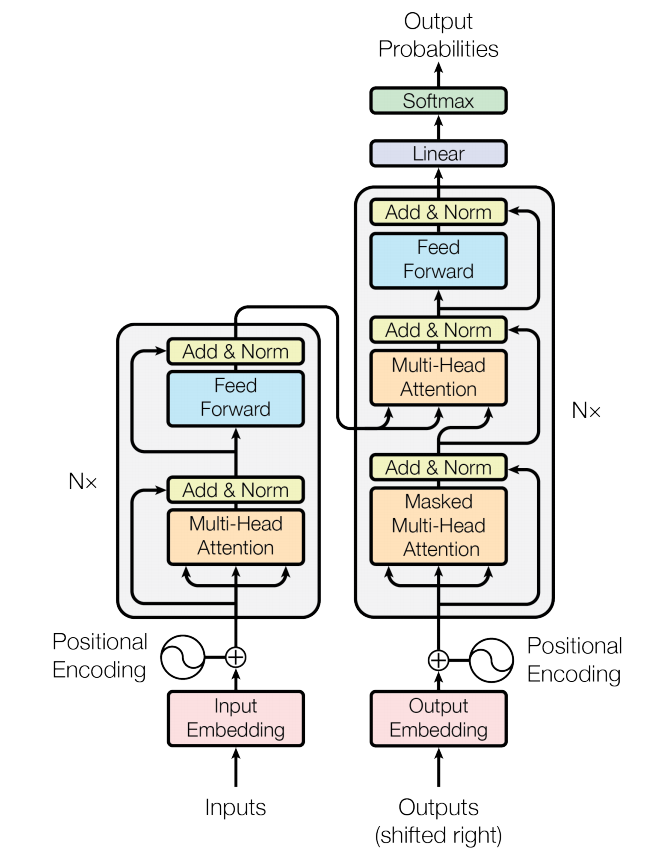
\includegraphics[width=0.95\linewidth]{imagenes/transformer-arquitectura.png} 
\caption{Arquitectura del \textit{transformer}.\\Fuente: \cite{NIPS2017_3f5ee243}}
\label{fig:arquitectura-transformer}
\end{wrapfigure}

\vspace{2mm}
En el \textbf{encoder} (parte izquierda de la Figura \ref{fig:arquitectura-transformer}), se encuentra un \textit{stack} de 6 capas. Cada una de estas, está compuesta por dos subcapas: una capa de \textit{Multi-Head Self-Attention} (un mecanismo de atención que se explicará más adelante); y una capa que contiene una red \textit{feed-forward} totalmente conectada. Cada una de estas subcapas, cuenta además con una conexión residual, que conecta la entrada de la subcapa con su salida de forma que puedan ser sumadas y normalizadas. Para facilitar la suma y normalización de entradas y salidas, todas las capas del modelo producen elementos de dimensión $d=512$. Antes de estas 6 capas, cada uno de los \textit{tokens} - elementos de la secuencia - de entrada (en la propuesta inicial, palabras), se convierten a vectores de dimensión $d$ a través de un \textit{embedding}\footnote{Operación que transforma, en el caso de la publicación original, palabras, en una representación numérica en un espacio vectorial donde las palabras con significado similar se encuentran próximas entre sí} previamente entrenado y se les añade una codificación posicional (en esta propuesta, generada a partir de funciones seno y coseno de distintas frecuencias) que aporta al modelo información sobre la posición de cada \textit{token} dentro de la secuencia inicial.

\vspace{2mm}
Por otro lado, en el \textbf{decoder} (parte derecha de la Figura \ref{fig:arquitectura-transformer}), se vuelve a encontrar un \textit{embedding} previamente entrenado que transforma las salidas del modelo desplazadas una posición. Al resultado de este \textit{embedding}, se le añade una codificación posicional similar a la del \textit{encoder}. A continuación, hay otro \textit{stack} de 6 capas, que esta vez está compuesto por las dos subcapas que están presentes en el \textit{encoder} (en este caso la capa de \textit{Multi-Head Self-Attention} es en realidad \textit{Multi-Head Masked Self-Attention} ya que se aplica una máscara para evitar que influyan en la red los \textit{tokens} siguientes al \textit{token} que se va a predecir), y una subcapa adicional de \textit{Multi-Head Cross-Attention}, situada entre las otras dos subcapas, donde las salidas de la subcapa de \textit{masked self-attention} del \textit{decoder} pueden acceder a las salidas del conjunto de capas del \textit{encoder}. (\textbf{La entrada de esta última capa de atención proviene de la última capa del \textit{encoder}, no de sus capas intermedias}). Por último, a la salida del \textit{stack} de capas del \textit{decoder}, se encuentra una transformación lineal (entrenada) y una función softmax para predecir la salida de la red.

% \paragraph{Mecanismos de atención}\mbox{}\\
\subsubsection{Mecanismos de atención}
% \todo[inline]{Hablar de los mecanismos de atención, y aunque se mencionen sus comienzos y sus aplicaciones en redes recurrentes y convolucionales, centrarse en que son la principal baza de los transformers y su "novedad", ya que solo funcionan con esto básicamente, si queda muy pegado aquí se puede sacar como subapartado de Redes Neuronales y distintas topologías.}

\vspace{2mm}
Los mecanismos de atención, presentados por primera vez en \cite{neuralmachinetranslationalignandtranslate}, buscan simular la atención cognitiva y han sido previamente empleados en redes recurrentes \cite{pmlr-v37-xuc15} y convolucionales \cite{7298685, 7410695} para aprender qué partes de la entrada son más relevantes en la tarea a completar. Sin embargo, en \cite{NIPS2017_3f5ee243}, con los \textit{transformers}, se propone por primera vez una arquitectura basada solamente en estos mecanismos. 
% \sout{De esta forma, se eliminan los sesgos cognitivos \cite{} que se han introducido en arquitecturas anteriores para facilitar su aprendizaje y mejorar su funcionamiento. Dichos sesgos cognitivos, son, por ejemplo, el uso de convoluciones para tratamiento de imágenes, donde se presupone que los elementos más cercanos a un píxel serán de mayor interés; o el uso de redes recurrentes secuenciales para procesamiento de lenguaje natural, donde se almacena toda la información que precede a un elemento de forma conjunta.} 
Las funciones de atención más empleadas son la atención aditiva \cite{neuralmachinetranslationalignandtranslate} y multiplicativa, siendo esta última la empleada en los \textit{transformers}, donde la atención se consigue a través de un producto escalar dentro de un bloque con múltiples cabezas llamado \textit{Multi-Head Attention}, elementos principales de los \textit{transformers}, que aparecen de dos formas distintas:
\begin{itemize}
    \item Bloques de \textit{Self-Attention}, en el \textit{encoder} y en el \textit{decoder}, con todas las entradas dentro de sus respectivas capas.
    \item Bloques de \textit{Cross-Attention}, en las capas del \textit{decoder}, con entradas provenientes del final de la pila de capas del \textit{encoder} y de la subcapa anterior del \textit{decoder}.
\end{itemize}
Cada una de las cabezas que componen estos bloques basan su funcionamiento en multiplicar sus entradas por una serie de matrices $W^V$, $W^K$ y $W^Q$ que son aprendidas durante el entrenamiento, de donde se obtienen, respectivamente, vectores \textit{Value} (V), \textit{Key} (K) y \textit{Query} (Q). Estos vectores, permiten que cada uno de los elementos de la secuencia de entrada, con el cálculo asociado a la atención (Figura \ref{fig:multi-head-attention}) soliciten a través de su vector \textit{Query} la información que determinen más importante de la secuencia. Esto se consigue al calcular el producto escalar de todos los vectores Q con todos los vectores K, que resultará mayor cuanto más alineados estén ambos vectores - mayor similitud entre las \textit{Queries} (consultas) y las \textit{Keys} (claves) -. A los resultados de estos productos escalares, se les aplica una función \textit{SoftMax} para asegurar que sumen una unidad y finalmente se multiplican por los vectores V para obtener el resultado final de la atención. Los resultados de todas las cabezas, se concatenan en una sola matriz para aprovechar al máximo el procesamiento en paralelo y atraviesan una última proyección linear.
% \todo[inline]{Hablar de la operación de atención y de como permite que se configuren los pesos automáticamente y acabar lo de softmax}
% \todo[inline]{En el anexo 1, hacer algo similar a \url{https://youtu.be/4Bdc55j80l8} + \url{https://jalammar.github.io/illustrated-transformer/}}
\begin{figure}[H]
\centering
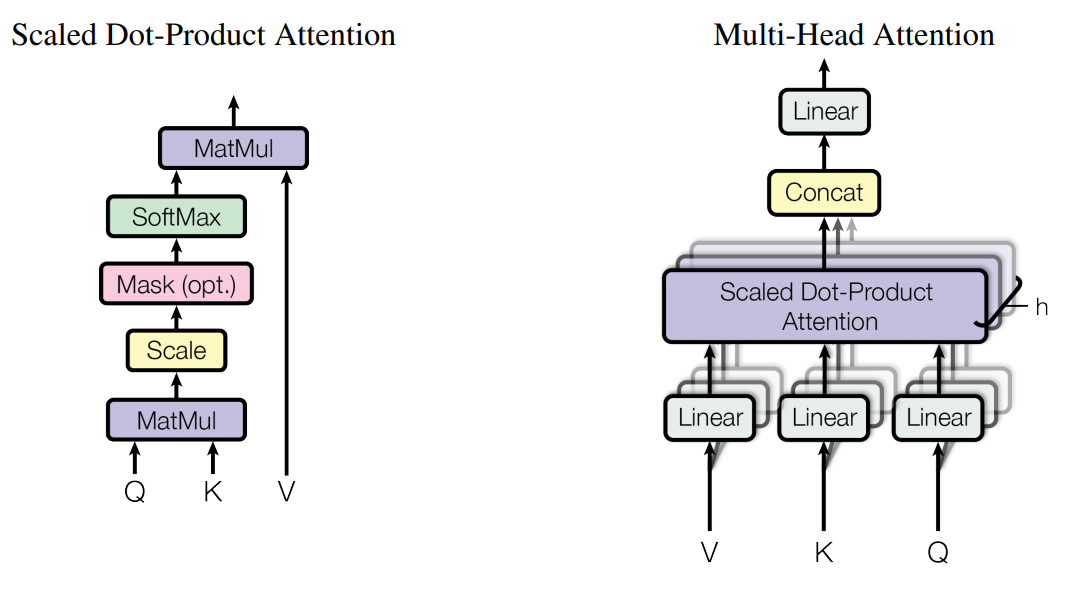
\includegraphics[width=0.65\linewidth]{imagenes/multi-head-attention.png} 
\captionsetup{width=.8\linewidth}
\caption{Producto escalar para el cálculo de la atención (izquierda) y bloque de \textit{Multi-Head Attention} (derecha). Fuente: \cite{NIPS2017_3f5ee243}}
\label{fig:multi-head-attention}
\end{figure}

Estos mecanismos de atención, sin embargo, son costosos, ya que tienen una complejidad $O(n^{2})$ tanto en tiempo como en memoria, siendo n el número de elementos de la secuencia de entrada (al bloque de atención). Es por esto por lo que han ido surgiendo una serie de propuestas para reducir dicha complejidad computacional, algunas de las cuales se exponen en la siguiente sección.



\subsubsection{Atención eficiente}
% \todo[inline]{Hablar de los distintos mecanismos que hay para reducir la complejidad computacional del self attention (se puede seguir la línea de \cite{2020arXiv200906732T} pero quitando los modelos que no nos interesen y profundizando en los papers de los modelos que sí. Ver si hay papers especificos de pruning en transformers que cuenten algo interesante ; https://arxiv.org/abs/1910.14488}



Para reducir los requisitos de memoria y el coste computacional de los \textit{transformers}, que tal y como se ha mencionado anteriormente, obtienen sus resultados gracias a los mecanismos de atención, pero que sin embargo son muy costosos computacionalmente, surgen distintas técnicas que buscan aproximar el resultado de la multiplicación de matrices que se lleva a cabo en los bloques de atención. Siguiendo el esquema propuesto en \cite{2020arXiv200906732T}, estas modificaciones de las capas de atención pueden agruparse en:

\todo[inline]{Hablar del performer en más detalle}

\subsubsection{Patrones fijos - Fixed Patterns (FP)}
En los patrones fijos, la longitud de la secuencia de entrada a los mecanismos de atención se reduce, por ejemplo: accediendo a ella en bloques de un tamaño determinado, en esto se basan \textbfit{Blockwise Attention} \cite{qiu-etal-2020-blockwise} y \textbfit{Local Attention} \cite{localattention}; accediendo a la secuencia en intervalos previamente definidos, como en \textbfit{Sparse Transformer} \cite{sparse-transformers} o \textbfit{Longformer} \cite{beltagy2020longformer} donde se emplean ventanas dilatadas o con un determinado \textit{stride} (zancada); o también empleando operaciones de \textit{pooling} para reducir la longitud de la entrada, en \textbfit{Compressed Attention} \cite{j.2018generating}.

% \subsubsection{Combinación de patrones - Combination of Patterns (CP)}
% Este grupo de métodos, se basa principalmente en la combinación de diferentes patrones de acceso a los elementos que componen la secuencia de entrada y aparece en \textbfit{Sparse Transformer} \cite{sparse-transformers} donde se combinan \textit{Local Attention} y \textit{strided attention} asignando la mitad de las cabezas del bloque de \textit{multi-head attention} a cada uno de los métodos. También aparece en \textbfit{Axial Transformer} \cite{ho2019axial}, donde la atención se aplica de forma independiente en cada uno de los ejes de la entrada (en este caso, el tensor de entrada debería ser multidimensional).

\subsubsection{Aprendizaje de patrones - Learnable Patterns (LP)}
Pese a ser similar a los dos casos anteriores ya que siguen basándose en diferentes formas de acceder a la secuencia de entrada para hacerla más dispersa, estos métodos son capaces de aprender en la etapa de entrenamiento del modelo qué patrones de acceso son más adecuados. Algunas de las propuestas que emplean este tipo de patrones son \textbfit{Reformer} \cite{Kitaev2020Reformer:}, que agrupa los elementos de la secuencia de entrada (\textit{tokens}) empleando una medida de similitud en grupos de elementos (para posteriormente aplicar el mecanismo de atención de forma independiente en cada grupo) o \textbfit{Routing Transformer} \cite{routingtransformer} que emplea k-medias para agrupar los \textit{tokens}, ambos modelos, reducen la complejidad a $O(n \log n)$. Dentro de estos modelos también destaca \textbfit{ResT} \cite{zhql2021ResT}, que está enfocado a imágenes y emplea convoluciones separables para reducir las dimensiones de las entradas al mecanismo de atención.

% \subsubsection{Memoria}
% Las técnicas que emplean elementos de memoria, reservan un modulo que puede acceder a todos los \textit{tokens} de la secuencia. De esta forma, este modulo puede recoger y almacenar información relevante del conjunto general de entrada. En \textbfit{Set Transformers} \cite{set-transformer} se introduce como un elemento de contexto temporal sobre toda la secuencia, también empleado en \textbfit{ETC} \cite{ainslie-etal-2020-etc} y \textbfit{Longformer} \cite{beltagy2020longformer}.

\subsubsection{Disminución de rango}
Este conjunto de arquitecturas, incluyen una proyección para conseguir una aproximación de la matriz resultante del cálculo de la atención, esta aproximación, pese a tener el mismo número de elementos (filas), obtiene una representación de los vectores menor (columnas), por lo que la dimensión de la matriz pasa de ser $n \times n$ a ser $n \times k$, con la consecuente disminución de coste computacional. El principal ejemplo de este tipo de arquitectura es \textbfit{Linformer}, \cite{wang2020linformer} que presenta una complejidad $O(n)$

\subsubsection{Kernels}
Por último, y aunque podrían entrar dentro del grupo de disminución de rango, existen enfoques que emplean kernelización en los mecanismos de atención para evitar el cálculo explicito de la matriz $n \times n$. Un ejemplo de este tipo de enfoques es el propuesto en \cite{kernel-transformer}, que de nuevo reduce la complejidad a $O(n)$.

%% La primera aparición de las depthwise separable convolutions parece ser en MobileNets: Efficient Convolutional Neural Networks for Mobile Vision Applications pero no lo tengo nada claro.
\subsubsection{Performer}
Este trabajo se centra en el mecanismo propuesto por .., el performer, para...

\subsection{Transformers para visión artificial - ViT}
A la hora de aplicar la arquitectura de los \textit{transformers} a procesamiento de imágenes, surge un problema importante. La complejidad del mecanismo de atención es $O(n^{2})$, siendo n el número de elementos en la secuencia de entrada, por lo que para una imagen de dimensiones $lado \times lado$, el número de píxeles que conformarían la secuencia de entrada al mecanismo de atención es $n = l^2$, disparando la complejidad de la atención a $O(l^{4})$. Para lidiar con este problema, se han propuesto distintas soluciones como limitar el mecanismo de atención al entorno de cada píxel (presentado en \textit{Image Transformers} \cite{image_transformer}) o aplicar convoluciones para reducir el tamaño de la secuencia de entrada \cite{detrfacebookdetectiontransformers}. 

Sin embargo, la solución propuesta en \textit{An Image is Worth 16x16 Words} con el \textit{Vision Transformer} \cite{image16x16words} es la que mejores resultados ha obtenido y por lo tanto aquella que más popularidad ha ganado como base de arquitecturas para otros problemas de visión artificial \cite{visiontransformersDPT, bhat2020adabins, chen2021transunet, liu2021Swin}. Esta solución, consiste en dividir la imagen original en fragmentos de tamaño fijo y convertir con una proyección cada fragmento en un vector de valores (\textit{embedding}). Estos vectores, son equivalentes al resultado del \textit{embedding} de palabras en la arquitectura original y se introducen al modelo como tal, es decir, cada fragmento extraído de la imagen correspondería a una palabra de una frase (Figura \ref{fig:vit}). Esta arquitectura, al ser inicialmente propuesta para realizar clasificación, solamente emplea el \textit{encoder} del \textit{transformer}.

\begin{figure}[H]
\centering
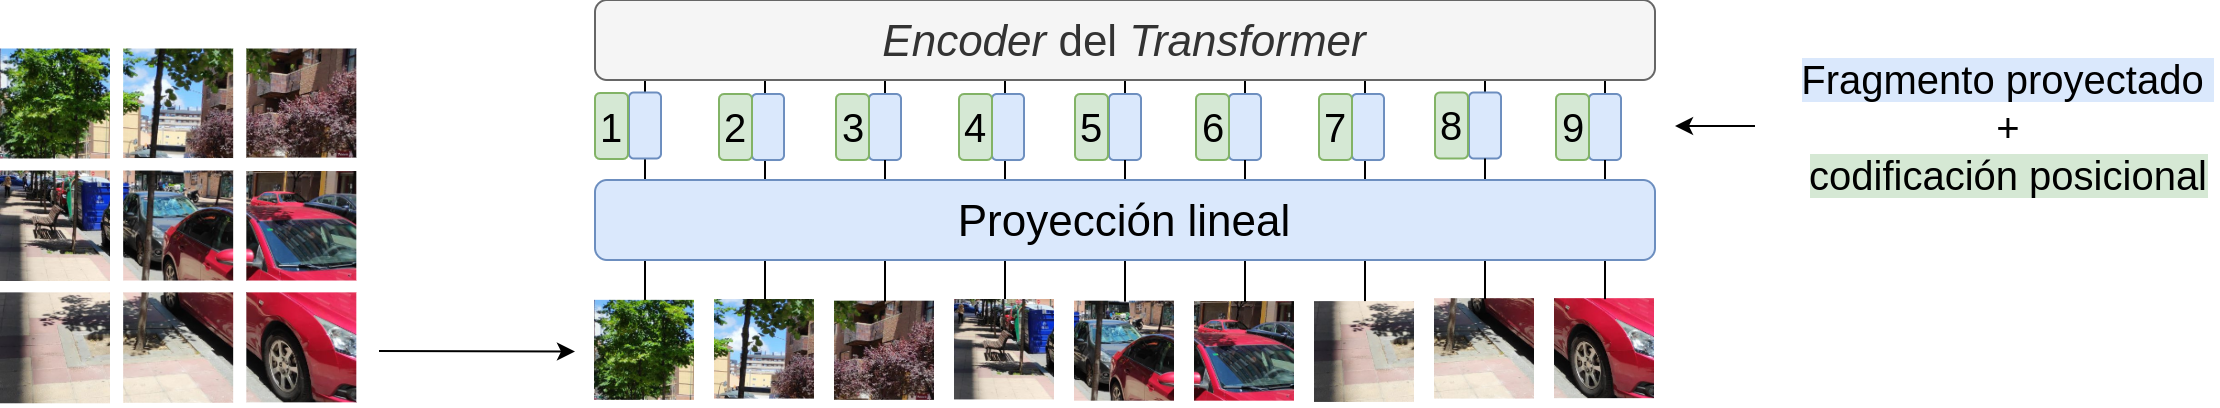
\includegraphics[width=1\linewidth]{imagenes/vit.png} 
\captionsetup{width=.8\linewidth}
\caption{\textit{Backbone} basado en fragmentos y proyección lineal del ViT. Figura inspirada en \cite{image16x16words}}
\label{fig:vit}
\end{figure}

En esta publicación, además, se presenta una variante del \textit{Vision Transformer}, el \textbfit{Hybrid Vision Transformer}. La diferencia entre esta arquitectura y la original es la sustitución del \textit{backbone} del ViT, es decir, de la separación en fragmentos y la proyección lineal, por una red convolucional de cuyos mapas de características se extraen los vectores que pasan a los bloques de atención (Figura \ref{fig:hybrid-vit}). Para formar estos vectores, en la implementación usada en este trabajo, se agrupan los mapas de características en función de sus píxeles, por lo tanto, si hay $n$ mapas de características, el píxel número 1 de cada uno de ellos formará un vector de dimensión n. De esta forma, la dimensión del vector viene dada por el número de mapas de características y el número de \textit{tokens} será equivalente al número de píxeles de los mapas de características (imágenes mayores conllevan un mayor número de \textit{tokens}).

\begin{figure}[H]
\centering
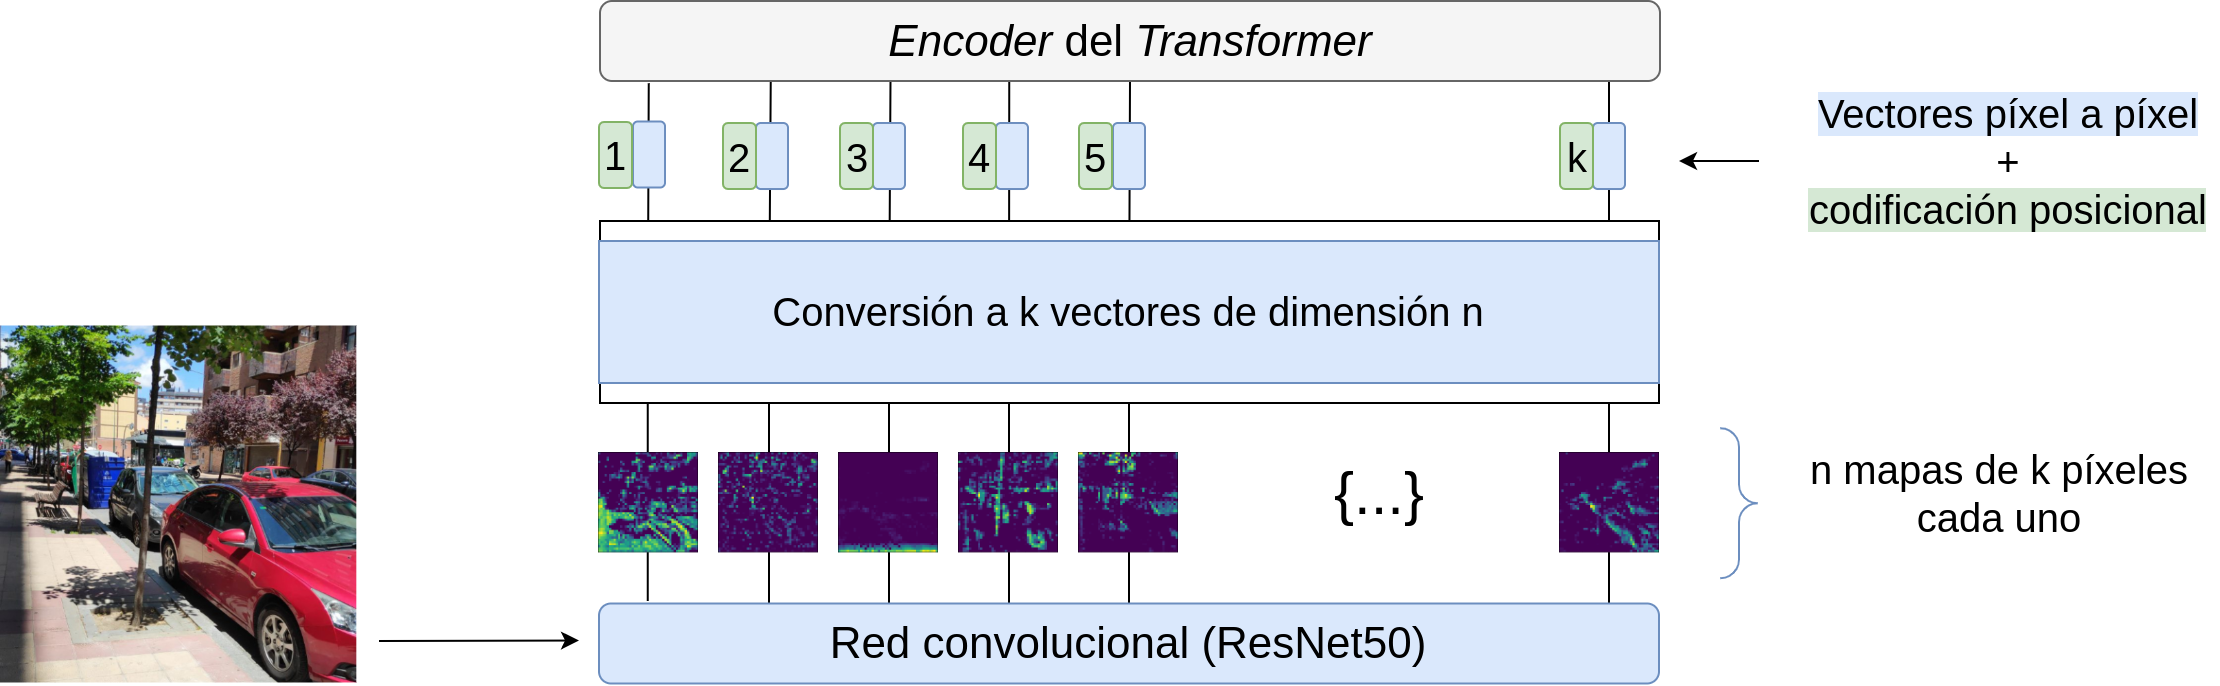
\includegraphics[width=1\linewidth]{imagenes/vit-hybrid.png} 
\captionsetup{width=.8\linewidth}
\caption{\textit{Backbone} convolucional del Hybrid-ViT.}
\label{fig:hybrid-vit}
\end{figure}

\subsection{Estimación de profundidades}
\todo[inline]{Repasar estos tres parrafo}
La estimación de profundidades, tanto cuando es llevada a cabo por humanos como por máquinas, consiste en detectar la distancia relativa entre todo aquello que se ve. Tal y como se ha mencionado en el capítulo de Introducción TODO, el cerebro humano se apoya principalmente en la disparidad existente entra las imágenes que capturan cada uno de los ojos (estereovisión), ya que las cosas que están más lejanas ven su posición menos alterada entre la vista de un ojo y de otro que las cosas cercanas. Sin embargo, el cerebro es también capaz de, a partir de nuestro conocimiento previo del mundo y nuestro entorno (pistas monoculares), estimar la profundidad en una sola imagen. 

Las técnicas de visión artificial tradicional (basadas en dos cámaras - visión estereoscópica) no pueden lidiar con este problema, por lo que la estimación monocular (con una sola cámara) es prácticamente imposible. Para este tipo de estimación (monocular), entran en juego los modelos de aprendizaje automático, que han demostrado una gran capacidad para explotar el conocimiento sobre el entorno en todo tipo de tareas, no siendo la estimación de profundidades diferente. 

A continuación, aunque haciendo especial hincapié en aquellos basados en aprendizaje automático, se enumeran los distintos enfoques existentes, incluyendo aquellos propios de la visión artificial tradicional, las soluciones \textit{hardware}, y las técnicas de aprendizaje profundo.

\subsubsection{Técnicas de estimación de profundidades} \label{estimacion-profundidades-sota}

La estimación de profundidades se ha intentado resolver de múltiples maneras \cite{Zhao_2020}. Dentro de estas metodologías, existen tres enfoques principales en función del tipo de \textit{software} o \textit{hardware} que se emplea.
\begin{itemize}
    \item \textbf{Soluciones geométricas}: Este grupo de métodos, extrae información de las restricciones geométricas que existen entre parejas de imágenes. Principalmente se agrupan en técnicas de \textit{SfM (Structure from Motion}) donde se reconstruye la tercera dimensión a partir de imágenes tomadas por una sola cámara en movimiento, y en técnicas de estereovisión, donde la profundidad se obtiene de la disparidad entre las imágenes capturadas por una pareja de cámaras con posiciones fijas entre sí y conocidas. Estos métodos, sin embargo, basan su funcionamiento en el emparejamiento de puntos claves (\textit{feature points}) que deben encontrarse en ambas imágenes, y por lo tanto necesitan texturas o formas características que poder emparejar.
    \item \textbf{Soluciones hardware}: Por otro lado, existen una serie de soluciones basadas en distintos sensores como son los LIDAR, las cámaras de tiempo de vuelo (ToF) o los escáneres de luz estructurada. Estas soluciones, no obstante, cuentan con ciertas limitaciones como son la densidad de sus capturas (representaciones de puntos dispersos en el caso del LIDAR\footnote{Por representaciones dispersas se entiende la captura de la profundidad en forma de una nube de puntos discretos separados entre sí, mientras que una representación densa tiene una mayor cantidad de puntos de información.}), la sensibilidad a la iluminación (en las cámaras ToF) o su rango de acción y la necesidad de un entorno controlado (luz estructurada).
    \item \textbf{Aprendizaje automático}: Debido a las restricciones de los métodos existentes y a los resultados obtenidos empleando aprendizaje automático en otros campos de la visión artificial, en los últimos años han surgido múltiples arquitecturas enfocadas a recuperar la profundidad a partir de imágenes. Este documento, pese a revisar superficialmente otras opciones, se centra en las \textbf{soluciones monoculares} debido al interés detrás de obtener una representación de la profundidad a partir de una sola cámara (por múltiples factores, coste, espacio, consumo, etc.).
\end{itemize}

% \todo[inline]{¿Contar un poco la historia siguiendo el review y luego ya profundizar? 
% Buen resumen para estirar -> \url{https://towardsdatascience.com/depth-estimation-1-basics-and-intuition-86f2c9538cd1}}

% https://openaccess.thecvf.com/content_CVPR_2020/papers/Johnston_Self-Supervised_Monocular_Trained_Depth_Estimation_Using_Self-Attention_and_Discrete_Disparity_CVPR_2020_paper.pdf

\subsubsection{Aprendizaje automático no supervisado}

Estas propuestas, ofrecen soluciones que emplean datos sin etiquetar debido a la dificultad que entraña la obtención de este tipo de datos. Normalmente, estas soluciones emplean secuencias (vídeos) de imágenes monoculares, extrayendo automáticamente a partir de estas una señal supervisora con distintos métodos. En \cite{zhou2017unsupervised} se propone una arquitectura que emplea una red neuronal para calcular la posición (y movimiento) de la cámara entre \textit{frames} consecutivos (\textit{ego-motion}), que a su vez se emplea para calcular la profundidad de la imagen. Sin embargo, da por hecho que ningún objeto ha cambiado de posición y que el entorno es estático. 

Esto, no es aplicable a entornos reales, por lo que surgen diferentes arquitecturas que generan máscaras, tanto basadas en redes neuronales \cite{zhou2017unsupervised, vijayanarasimhan2017sfmnet} como en técnicas geométricas \cite{geo_mask_egomotion, monodepth}, para lidiar con los objetos dinámicos. Otros enfoques, con la misma idea subyacente, sustituyen la red de estimación de posición con métodos de odometría visual\footnote{La odometría agrupa aquellas técnicas que estiman el cambio de posición a partir de las lecturas de sensores. En el caso de la odometría visual, estos cambios de posición se estiman empleando principalmente imágenes capturadas por una cámara.} tradicional \cite{visualodometryunsupervised}, que puede aportar posiciones más exactas y mejorar el funcionamiento final. Por último, algunos enfoques calculan elementos adicionales como por ejemplo el flujo óptico de la escena (cálculo de los patrones de movimiento para cada punto de la imagen) que aporta información relevante sobre la posición relativa de los objetos \cite{vijayanarasimhan2017sfmnet, geonet}. 

\subsubsection{Aprendizaje automático semisupervisado}

Debido a la escasez de datos etiquetados, también son populares los enfoques semi supervisados. Estas soluciones, emplean información parcial como señal supervisora, que complementan con información no etiquetada. Algunos ejemplos característicos de este tipo de aprendizaje son: 
\begin{itemize}
    \item Síntesis artificial de parejas a partir de imágenes monoculares para emplear técnicas de estereovisión, entrenando los modelos con parejas de imágenes obtenidas por conjuntos de cámaras preparados para estéreo \cite{monocularstereosynthesis, single-view-stereo-matching}.
    \item Generación de los mapas de disparidad entre parejas de imágenes para estereovisión \cite{importancestereo, deep3d}, donde la señal supervisora es la disparidad obtenida mediante técnicas tradicionales de estereovisión.
    \item Utilización de datos etiquetados de forma dispersa (frecuentemente obtenidos con dispositivos LIDAR), que o bien emplean imágenes no etiquetadas para densificar dichas representaciones \cite{lidarcompletion, sparse-to-dense, hu2020PENet} o añaden la información del LIDAR en la función de perdidas para después inferir a partir de imagen monocular \cite{lidarlossfunction}.
\end{itemize}

\subsubsection{Aprendizaje automático supervisado} \label{aprendizaje-supervisado}
% Ver CRFs en condiciones
Pese a la dificultad para obtener datos etiquetados correctamente, los enfoques supervisados siguen siendo los que mejores resultados ofrecen y por lo tanto han sido y siguen siendo extensamente estudiados. El primero de estos modelos fue propuesto en \cite{eigen-multi-scale}, y empleaba dos conjuntos de capas, uno para generar una estimación tosca de la profundidad y otro para refinar esa primera estimación. Enfoques posteriores propusieron modificaciones en la función de perdidas para fomentar la consistencia en las predicciones \cite{surfacenormals} a través del cálculo de los gradientes de la diferencia entre el resultado y el objetivo. Otra función de de perdidas popular es la perdida \textit{Berhu} \cite{zwald2012berhu}. Además de aquellos basados en arquitecturas \textit{encoder-decoder}, también hay propuestas con arquitecturas de aprendizaje adversario \cite{gan} donde el discriminador trata de distinguir entre la profundidad generada y la real \cite{gan-depth}.

% DPT ajusta mínimos cuadrados la predicción con el ground truth para sacar un factor de escala, AdaBins da profundidades en metros.
Todas estas soluciones, basan su funcionamiento en redes convolucionales, sin embargo, los \textit{transformers} han presentado muy buenos resultados en los últimos años y también se han propuesto soluciones que emplean estas arquitecturas. Entre estos modelos, destacan:
\begin{itemize}
    \item \textbfit{Dense Prediction Transformers}: Propuesto en \cite{visiontransformersDPT}, emplea como \textit{backbones} los distintos modelos propuestos en \cite{image16x16words}, de donde se extraen representaciones intermedias de diferentes resoluciones que posteriormente se fusionan empleando capas convolucionales. Esta red, cuenta con dos cabezas, una pre-entrenada para estimación de imágenes monocular y otra para segmentación semántica. Este modelo, proporciona distancias relativas, es decir, no aporta información métrica.
    \item \textbfit{AdaBins}: Presentado en \cite{bhat2020adabins}, también emplea como base los \textit{vision transformers} propuestos en \cite{image16x16words}. A diferencia del modelo anterior, \textit{AdaBins (Adaptative Bins)} propone un bloque adicional que clasifica cada píxel en un histograma de profundidades cuyas barras (\textit{bins}) son parametrizadas (centro y rango) dinámicamente para cada imagen. El resultado final se consigue con la suma ponderada de la predicción de pertenencia a cada barra y el valor medio de dicha barra, consiguiendo así una estimación de profundidad más suavizada. A diferencia del anterior, aunque con ligeramente peores resultados, \textit{AdaBins} sí que proporciona distancias en metros.
\end{itemize}
Los tiempos de inferencia de estos modelos han sido evaluados en distintos dispositivos y se presentan en la sección \ref{resultados}.


\subsubsection{DPT}
\textbf{Introducción}

\todo[inline]{Añadir citas aquí}
Las arquitecturas de estimación de profundidades se basan en redes convolucionales, normalmente de tipo \textit{encoder-decoder}. Las líneas de investigación actuales se centran en el \textit{decoder} y sus estrategias de agregación de información, sin embargo, DPT centra su estudio en la modificación del \textit{encoder}, debido a la gran influencia que tiene este en la información que llega a la segunda parte de la red.

\todo[inline]{Esto puede que haya que moverlo a otra zona del documento para argumentar por qué se usan transformers y no redes convolucionales}
En el artículo, argumentan que los \textit{backbones} convolucionales reducen dimensionalmente la imagen de forma progresiva para extraer sus mapas de características con distintos niveles de abstracción mientras se mantienen razonables los requisitos computacionales y de memoria. Este tipo de operaciones, que han ofrecido muy buenos resultados en todo tipo de tareas de visión artificial, presentan ciertos inconvenientes críticos en la estimación de profundidades, principalmente la resolución y granularidad de los mapas de características extraídos. Esto, es un problema debido a que para estimar la profundidad de una imagen con la mayor exactitud posible, sería conveniente que los mapas de características extraídos de la imagen mantuvieran su resolución original (o cercana a esta).

Pese a que se han planteado distintos métodos para reducir la perdida de resolución en los mapas de características (emplear imagenes más grandes, convoluciones dilatadas, skip connections, conexión de representaciones internamente, etc.) \todo[inline]{citar todo esto si se queda}, esta perdida de granularidad es inherente a la operación de convolución tál y como se aplica en este tipo de redes. Para solucionar esto, DPT emplea transformers (en concreto, vision transformers) como \textit{backbone} para evitar una reducción explicita de la resolución de las características extraidas de la imagen y ampliar el campo receptivo con el que opera la red (es posible usar información de toda la imagen en cualquier etapa de la arquitectura - campo receptivo global -, mientras que las capas convolucionales tienen campos receptivos locales mucho menores).

\todo[inline]{El trabajo previo repartirlo por el fundamento teórico}

\textbf{Arquitectura}

Como ya se ha comentado, DPT tiene por \textit{backbone} un vision transformer (ViT), es decir, fragmenta la imagen original en parches, extrae un \textit{embedding} de cada parche, y pasa este conjunto de vectores como entrada al transformer, de forma similar a como se pasarían los \textit{embeddings} de palabras cuando se aplican estas arquitecturas a texto. El artículo proporciona dos versiones de DPT en función del vision transformer que emplean. La primera tiene por \textit{backbone} una arquitectura ViT large (proyección lineal, x capas,,,) \todo[inline]{hablar del número de capas de vit large}; y la segunda emplea un ViT Hybrid (que emplea una ResNet50 para extraer el \textit{embedding} de los parches iniciales).

En la parte del \textit{decoder}, se forman representaciones de distintas resoluciones en forma de imagen a partir de los tokens que se encuentran en ciertas capas del transformer. Estas representaciones, se combinan de forma progresiva para obtener la predicción final de la red (la estimación de profundidad para cada píxel).

La operación que convierte los \textit{tokens} de capas intermedias del \textit{transformer} en imágenes se define de la siguiente manera:

\todo[inline]{Ecuación y probablemente imagen en algún sitio del decoder}

\begin{enumerate}
\item{Read: Integración del readout token: ...}
\item{Concatenate: ...}
\item{Resample: ...}
\end{enumerate}

Una vez se han extraido estas representaciones intermedias a diferentes resoluciones, se fusionan empleando una arquitectura de tipo RefineNet \todo[inline]{citar y explicar la arquitectura}. El resultado de este último bloque, es una imagen con la mitad de resolución que la imagen de entrada que pasa por una cabeza entrenada para proporcionar la predicción final. 

Los modelos publicados, han sido entrenados en MIX 6, un dataset elaborado por Intel ampliando MIX 5, también empleado por la empresa en MiDas, el modelo precursor de DPT. Este dataset está compuesto por los siguientes datasets:
\todo[inline]{Hablar de los dataset de entrenamiento y test, citandoles y haciendo una tabla de número de imágenes, espacio, etc. También se puede mencionar que hay algunos que son dificiles de conseguir debido a las leyes actuales que no se han publicado.}

Además de los modelos entrenados en MIX 6, se proporcionan los parámetros de la variante DPT-Hybrid tras realizar un \textit{fine tuning} en los conjuntos de entrenamiento de los datasets NYU Depth v2 y KITTI (cuyos conjuntos de test se emplean posteriormente en este trabajo para comparar los resultados de los distintos modelos resultantes). 

\todo[inline]{Hablar del proceso de entrenamiento que llevan a cabo en el paper de DPT?}

\todo[inline]{Copiar los resultados del paper en ambos datasets y aclarar que esos resultados son los que se presentan en el paper, después en la sección de resultados pondremos los que consigamos nosotros con un proceso de prueba más cercano a lo que sería un entorno de producción, sin dobles predicciones ni cosas similares.}

\subsection{Optimización de modelos}
% \todo[inline]{https://heartbeat.fritz.ai/the-5-algorithms-for-efficient-deep-learning-inference-on-small-devices-bcc2d18aa806}

% \todo[inline]{Hablar de las formas no especificas con las que se pueden acelerar las redes neuronales, sería mencionar las de la presentación de la quinta reunión hablando un poco de cada una de ellas. También se podría meter un pequeño apartado de hardware hablando de TPUs y FPGAs, habría que ver como se cuadra y como encaja con el resto del apartado. Esto puede que para el TFM haya que recortarlo un poco también de cara a acotar un poco el estudio si no se va a hacer nada de esto (centrarnos en velocidad sin entrar en restricciones de memoria, por ejemplo)}
% \paragraph{Basadas en Hardware}\mbox{}\\
% \todo[inline]{Mencionar que hay TPUs (ASICs), GPUs, ... A lo mejor es conveniente sacar esto a un apartado de aceleración por hardware distinto de los mecanismo de eficiencia. La clasificación que hacen en las diapositivas de la clase de Stanford está bastante bien, se puede hablar de las cuatro cosas centrandonos en software para inferencia. ; \url{https://youtu.be/eZdOkDtYMoo} ; \url{http://cs231n.stanford.edu/slides/2017/cs231n_2017_lecture15.pdf}}

% \paragraph{Basadas en Software}\mbox{}\\
Los modelos de aprendizaje automático más novedosos, son cada vez más grandes, lo que generalmente conlleva un tiempo de entrenamiento y de inferencia mayor, así como unos requisitos de memoria y consumos de energía mayores. Para solucionar algunos de los problemas asociados, como por ejemplo la necesidad de proporcionar buenos resultados con restricciones temporales o restricciones de \textit{hardware} (modelos embebidos, dispositivos móviles, etc.) han ido surgiendo a lo largo de los años una serie de soluciones que tratan estos aspectos, buscando siempre perjudicar lo mínimo posible los resultados de los modelos originales. A continuación, se presentan algunas de las más generales, aplicables en una gran variedad de arquitecturas.
% \todo[inline]{Hablar de las que son aplicables a más de un tipo de red, si encontramos alguna que sea solo para convolucionales, por ejemplo, podemos mencionarlas todas de corrido diciendo que existen también técnicas que son aplicables a arquitecturas concretas pero que dado que nos vamos a centrar en los transformers no se entra en esto.}

% \todo{Ver en el correo de gmail de papers tfm practicas el deep compression}

\begin{itemize}
    \item \textbf{Poda / Pruning}: Consiste en eliminar de los modelos aquellas conexiones o neuronas que son redundantes o menos relevantes para la red, con el objetivo principal de reducir el tamaño del modelo, ya que las redes neuronales suelen estar sobredimensionas y son redundantes. Al reducir el tamaño del modelo, aumentar la velocidad con la que se realiza la inferencia\footnote{Dependiendo de las técnicas utilizadas para llevar a cabo la poda, pueden aparecer limitaciones en el hardware de uso general para trabajar con matrices dispersas, pero existen soluciones tanto hardware como software para trabajar con estos datos.} sin sacrificar la exactitud del modelo en exceso. Siguiendo la clasificación presentada en \cite{vadera2020methods}, los métodos más empleados de poda se pueden agrupar en dos grandes grupos: Basados en magnitud y basados en sensibilidad.
    \begin{itemize}
        \item \textbf{Métodos basados en magnitud}:  Estas técnicas, eliminan los parámetros basándose en su valor o en la influencia que tienen en la siguiente capa. Por ejemplo, un peso con un valor muy próximo a cero apenas influirá en la capa siguiente, y por lo tanto puede eliminarse. Estas técnicas, suelen llevarse a cabo eliminando parámetros y reentrenando la red de forma iterativa, repitiendo este proceso hasta encontrar un equilibrio entre reducción de tamaño y pérdida de exactitud. Han et al. \cite{NIPS2015_ae0eb3ee} presentaron, empleando este entrenamiento recursivo, resultados donde se eliminan más de un 90\% de los parámetros aumentando solamente en unas décimas el porcentaje de error en comparación con los modelos sin podar. 
        % En este trabajo, también se probaron dos puntos importantes: la regularización L1 proporciona mejores resultados antes del reentrenamiento, pero sin embargo la regularización L2 genera mejores resultados después de el reentrenamiento; y que estos entrenamientos sucesivos del modelo (siempre con un \textit{learning rate} menor que en el entrenamiento inicial), convergen en mejores valores para los pesos que han permanecido sin podar si se parte de los resultados del primer entrenamiento y no se reinicializan aleatoriamente \todo{Ver lo de la inicialización con pesos de entrenamientos posteriores y puede que quitar estos dos últimos puntos}. 
        Además de la poda de conexiones y neuronas, existen también distintas técnicas destinadas a podar con una menor granularidad, por ejemplo, mapas de características y filtros. Algunas de estas técnicas incluyen las basadas en la varianza entre canales \cite{7303876} o en el número medio de ceros que tienen los mapas de características \cite{2016arXiv160703250H} entre otras.
        
        \item \textbf{Métodos basados en sensibilidad}: Estos métodos, a diferencia de los basados en magnitud, buscan analizar el efecto de la modificación de los pesos en la función de perdida. Para ello, suelen centrarse en aproximar los cambios en la función de perdida a través de una serie de Taylor. Esta serie de Tylor, incluye una matriz hessiana, que se obtiene a partir de las segundas derivadas de la perdida respecto de los pesos. 
        % \todo{Poner las dos ecuaciones?} 
        Dado que el cálculo de la matriz hessiana es computacionalmente costoso, Lecun et al. en \textit{Optimal Brain Damage (OBD)} \cite{NIPS1989_6c9882bb} ignora los elementos que no están situados en la diagonal de la matriz, reduciendo la complejidad del cálculo considerablemente. Posteriormente, Hassibi et al. plantearon no descartar dichos valores en \textit{Optimal Brain Surgeon (OBS)} \cite{NIPS1993_b056eb15} pero sus cálculos son prohibitivos con el número de parámetros de las arquitecturas actuales. Estas series de Taylor, también se han empleado para la poda de canales y mapas de características en redes convolucionales, tanto con aproximaciones de primer orden \cite{molchanov2017pruning} como de segundo orden \cite{pmlr-v97-wang19g}. 
        % Por último, cabe mencionar que existen también métodos que emplean agentes en cada capa para aprender que filtros eliminar para maximizar una función dada por el rendimiento y el tamaño de la red \cite{8354187}.
        
        % \item \textbf{Métodos de \textit{clustering} y semejanza}: Mirar a ver si estos tienen algo que ver con el weight sharing, y o mencionarlos muy por encima o no mencionarlos.
    \end{itemize}
    % \item \textbf{Weight sharing}: Lorem ipsum.
    \item \textbf{Quantization}: La cuantificación tiene como objetivo convertir los parámetros de las redes almacenados en 32 bits en representaciones más pequeñas como son los números enteros (normalmente en 8 bits). Esta transformación, conlleva una perdida de calidad en los resultados de los modelos, pero reduce sus requisitos de memoria y acelera la inferencia de resultados. Esta aceleración viene dada por la velocidad a la que se pueden realizar operaciones con números enteros comparado con las operaciones con números en coma flotante. Existen principalmente tres tipos de cuantificación, dinámica, estática (estas dos se aplican sobre un modelo ya entrenado) y durante el entrenamiento (\textit{Quantization Aware Training}).
    \begin{itemize}
        \item \textbf{Cuantificación dinámica}: En este caso, no solo se convierten los pesos del modelo ya entrenado a enteros, sino que también se transforman las activaciones buscando los parámetros de dichas conversiones de forma dinámica durante la inferencia. Este tipo de cuantificación no requiere de datos pero sin embargo no es tan rápida como las otras dos al tener que realizar las transformaciones durante la inferencia.
        \item \textbf{Cuantificación estática}: De forma similar al caso dinámico, las activaciones de las capas se cuantifican durante la inferencia, sin embargo, en este caso una vez se ha entrenado la red se le pasan bloques adicionales de datos con los que se estiman los parámetros de estos procesos de cuantificación para acelerar la inferencia cuando se haya desplegado el modelo. De esta forma, pese a que es necesario tener datos adicionales (no hace falta que estén etiquetados), se alcanza una mayor velocidad de inferencia.
        \item \textbfit{Quantization Aware Training}: Por último, esta opción tiene en cuenta la cuantificación durante todo el proceso de entrenamiento simulando el efecto de la cuentificación en los pesos y activaciones de forma que influyan en la función de perdidas (las operaciones durante el entrenamiento siguen haciéndose en coma flotante). Este método, debido a la consideración de la cuantificación durante el entrenamiento, resulta en una inferencia más rápida y resultados superiores a los de los métodos anteriores. Sin embargo, no siempre es aplicable al requerir el entrenamiento del modelo.
    \end{itemize}
    % \todo[inline]{Esto se puede mirar en las referencias que hace Method for Pruning Deep Neural Networks al principio de la página 3 ; https://leimao.github.io/article/Neural-Networks-Quantization/}
    \item \textbfit{Weight clustering}: El \textit{clustering} de pesos, o \textit{weight sharing}, agrupa los pesos del modelo en un número determinado de \textit{clusters} para asignar a cada peso el valor del centroide de su grupo correspondiente. De esta forma, se reducen los requisitos de memoria del modelo, ya que solamente es necesario almacenar los índices que apuntan al vector de centroides, que al ser números enteros se pueden representar con un número de bits mucho menor (por ejemplo, en 8 bits, reduciendo el tamaño de la matriz de pesos original (cada uno 32 bits) a un cuarto de su tamaño).
    
    \item \textbf{Mixed-precision training}: Propuesto por primera vez en \cite{micikevicius2018mixed}, el entrenamiento con precisión mixta almacena los pesos, activaciones y gradientes en formato de coma flotante de media precisión (16bits - IEEE 754) en vez de simple precisión (32 bits). De esta forma, sin perder precisión, se reducen a cerca de la mitad los requisitos de memoria en el entrenamiento, que además se ve acelerado en las últimas arquitecturas de GPUs. 
    %Para esto se llevan a cabo tres estrategias: Mantener una copia maestra de los pesos almacenada en FP32, escalar el resultado de la función de perdida y acumular ciertos resultados en FP32.
    % \begin{itemize}
        % \item \textbf{Copia maestra de los pesos en FP32}: A pesar de que en el \textit{forward} y \textit{backward pass} del entrenamiento se usan valores FP16, se debe almacenar una copia maestra en FP32 de los pesos, que son los empleados en el optimizador para multiplicar por gradientes y \textit{learning rates}. Si bien es cierto que esto aumenta los requisitos de memoria de los pesos en un 50\%, el impacto en el conjunto global es mucho menor ya que el consumo de memoria durante el entrenamiento está dominado por las activaciones de cada capa.
        % \item \textbf{Escalado de la perdida}: Por otro lado, al calcular los gradientes de los pesos, también podrían resultar demasiado pequeños como para representarse correctamente en FP16. Esto se soluciona escalando el resultado de la función de perdidas al finalizar el \textit{forward pass} y antes de empezar el \textit{backpropagation} para que tengan una magnitud mayor. De esta forma, todos los gradientes resultan escalados por la misma magnitud al derivar y basta con reescalarlos a FP32 una vez finalizado el \textit{backpropagation} y antes de la etapa del optimizador.
        % \item \textbf{Precisión aritmética}: Para poder asegurar los mismos resultados que con FP32, las multiplicaciones parciales de los productos escalares y las reducciones (sumas de todos los elementos) de vectores FP16 tienen que acumularse en valores FP32, que antes de escribirse en memoria se convierten a FP16.
    % \end{itemize}
    % \item \textbf{Destilación de conocimiento}: Lorem ipsum 
\end{itemize}

% \subsection{Conjuntos de datos?}
% \todo[inline]{No en el marco teórico, se van a usar tanto realmente como para dedicarles una sección? es posible que sobre.}

\clearpage










----

% Dado que este trabajo se centra en los modelos basados en \textit{transformers}, una arquitectura de red neuronal relativamente nueva (2017), se describen primero estas arquitecturas.
\subsection{Redes neuronales - Transformers}
%\paragraph{Transformers para visión}\mbox{}
\subsubsection{Transformers para visión}
% \todo[inline]{Esto es susceptible de moverse a la sección de estado del arte, se podría introducir las técnicas generales sin centrarnos en los papers.}
% \subsubsection{Mecanismos? de eficiencia} \label{eficiencia-general}
\subsection{Estimación de profundidades}
\subsection{Técnicas de mejora de eficiencia} \label{eficiencia-general}
\subsection{Estimación de profundidades eficiente}
%\todo[inline]{Hablar de:\\
%\url{https://github.com/intel-isl/MiDaS/tree/master/ros} - es convolucional aunque midas sea ahora transformer, atender a las versiones.}
% \todo[inline]{Preguntar lo del link a towardsdatascience, no me convence pero es una explicación mucho más clara que en el paper de mobilenets}
% \todo[inline]{Meter imágenes de las arquitecturas de cada uno, si no es en la memoria de practicas (por reducir), en el TFM}
Empleando (junto a otras) las técnicas de optimización comentadas, se han propuesto distintos modelos que aceleran o fusionan distintas arquitecturas dedicadas a la estimación de profundidades, aparentemente, todos convolucionales. El estudio realizado, si bien es cierto que existen modelos dedicados a la aceleración y reducción de tamaño para hacer estimación de profundidades basados en imágenes de estéreo con aprendizaje supervisado \cite{faststereodepth} o que emplean imágenes monoculares con aprendizaje no supervisado \cite{pydnet18, mininet}, se centra en aquellos que funcionan sobre imágenes monoculares y cuyo aprendizaje ha sido de tipo supervisado. Los principales modelos con estas características son:
\begin{itemize}
    \item \textbfit{FastDepth} \cite{icra_2019_fastdepth}: Basado en una arquitectura de tipo \textit{encoder-decoder} convolucional, \textit{FastDepth} emplea como \textit{encoder} la red \textit{MobileNet} \cite{mobilenets} y construye el \textit{decoder} con convoluciones separables en profundidad\footnote{Partiendo de que las convoluciones separables permiten descomponer el \textit{kernel} en \textit{kernels}  de menor dimensión, las convoluciones separables en profundidad, permiten descomponer el \textit{kernel} original por canales, reduciendo drásticamente el número de operaciones. Se puede encontrar más información sobre el funcionamiento de este tipo de convoluciones en \cite{mobilenets}.} (\textit{depthwise separable convolutions}) y bloques de \textit{upsample} mediante interpolación de tipo vecino más cercano para aumentar el tamaño del resultado hasta el tamaño de la imagen de entrada. Posteriormente, se poda la red con \textit{NetAdaptV1} \cite{eccv_2018_yang_netadapt}, un algoritmo capaz de adaptar automáticamente una red al presupuesto de memoria definido. Algo que los autores destacan en el artículo, es cómo normalmente se optimiza solamente el \textit{encoder} en este tipo de arquitecturas, mientras que su propuesta optimiza también el \textit{decoder}.
    
    \item \textbfit{MobileDepth} \cite{wang2020mobiledepth}: De forma similar al modelo anterior, \textit{MobileDepth} se basa en una arquitectura \textit{encoder-decoder} convolucional. En este caso, el \textit{decoder} está compuesto por una red \textit{RegNetY06} \cite{regnety} mientras que el \textit{decoder} está formado por bloques \textit{split-concatenate shuffle}, inspirados en \textit{ShuffleNet v2} (este tipo de bloque, cuenta con una modificación de las convoluciones separables en profundidad que lo hace ligeramente más rápido). Este modelo, evaluado en NYU Depth v2 \cite{nyudepthv2}, presenta mejores resultados que \textit{FastDepth} (Tabla \ref{tab:comparacion-fastdepth-mobile-depth}), pero es cerca de un 10\% más lento (55ms y 62ms en CPU).
    
    \begin{table}[H]
    \centering
    \begin{tabular}{@{}ccccc@{}}
    \toprule
    Red                            & MACs {[}G{]}  & RMSE           & $\delta1$ & CPU {[}ms{]} \\ \midrule
    \textit{FastDepth (sin podar)} & 0.74          & 0.599          & 0.775                  & \textbf{55}  \\
    \textit{MobileDepth}           & \textbf{0.70} & \textbf{0.497} & \textbf{0.827}         & 62           \\ \bottomrule
    \end{tabular}
    \caption{Resultados comparativos presentados en \cite{wang2020mobiledepth}, siendo MAC el número de operaciones de multiplicación y acumulación, RMSE la raíz del error cuadrático medio, $\delta1$ la exactitud bajo umbral \cite{depth-estimation-metrics} y CPU el tiempo de inferencia.}
    \label{tab:comparacion-fastdepth-mobile-depth}
    \end{table}
    % \todo[inline]{Hablar de las métricas en el TFM\\
    % \url{https://arxiv.org/pdf/1805.01328.pdf}\\
    % \url{https://ylatif.github.io/papers/IROS2016_ccadena.pdf} \cite{depth-estimation-metrics}\\}
    
    % \item \textbfit{Domain Adaptation via Image Style Transfer} \cite{realtime-monocular-style-transfer}: En otro marco distinto a los dos enfoques anteriores, esta arquitectura realiza la inferencia en 22.7ms, si bien es cierto que lo consigue con una tarjeta gráfica de escritorio (GTX 1080 Ti) y no con CPUs móviles como en los casos anteriores. Este modelo, basa su entrenamiento en imágenes generadas sintéticamente y soluciona el problema del cambio de dominio (pasar de imágenes artificiales en el entrenamiento a imágenes reales en la inferencia) empleando transferencia de estilo desde una imagen real a las imágenes generadas sintéticamente. En cuanto a la red, se emplea una arquitectura de tipo GAN (\textit{Generative Adversarial Network}) \cite{gan}.
    % \todo[inline]{Ampliar esto un poco? Es el menos interesante y el que más largo está de momento pero queda un poco corto la parte de la arquitectura.}
\end{itemize}



\clearpage

\section{Material y Métodos}

En este tercer capítulo se introducen los materiales empleados para la realización del Trabajo Fin de Máster, tanto a nivel informático (\textit{software} y \textit{hardware}) como a nivel de datos. Después, se detalla las metodología seguida durante el proyecto para definir los distintos modelos de que se entrenarán, y por último se describen las herramientas empleadas durante el proceso de evaluación.

\subsection{Software}

\textbf{Lenguaje de programación y librerías}

Para el desarrollo de este proyecto, se ha elegido como lenguaje de programación \textbf{Python 3.7.10} debido a su ecosistema de librerías y código abierto orientado al aprendizaje profundo. Junto con Python, se han empleado principalmente una serie de librerías y paquetes que pueden distinguirse en dos grupos: 
\begin{itemize}
\item Uso de CPU: \textbf{Numpy 1.20} \cite{numpy}, para trabajar con matrices y acelerar operaciones matemáticas; \textbf{OpenCV 4.5.2} \cite{opencv_library}, para la carga y manipulación de imágenes antes de convertirlas en tensores, \textbf{fvcore 0.1.5} \cite{fvcore}, para calcular el número de operaciones de los modelos de aprendizaje profundo, y \textbf{Matplotlib 3.4} \cite{matplotlib} / \textbf{Seaborn 0.11} \cite{seaborn}, para graficar resultados y otras figuras de este documento.
\item Uso de GPU: \textbf{PyTorch 1.9.0} \cite{pytorch}, para la creación, modificación, entrenamiento y evaluación de modelos de aprendizaje profundo acelerados por \textit{hardware} (es decir, ejecutados en GPUs); \textbf{timm (PyTorch Image Models) 0.4.9} \cite{timm}, desarrollado y mantenido por Ross Whigtman, que pone a disposición del usuario un gran número modelos del estado del arte preentrenados e implementados en PyTorch; el \textbf{repositorio de DPT} \cite{visiontransformersDPT}, modelo que se modifica a lo largo del proyecto; y por último, el repositorio \textbf{performer-pytorch 1.1.3} \cite{pwperformer} de Phil Wang, que ofrece una implementación, también en PyTorch, de la arquitectura Performer y sus mecanismos de atención.
\end{itemize}

Algunas de estas librerías tienen alternativas que podrían haberse empleado perfectamente en este proyecto. La elección más importante es probablemente el uso de PyTorch frente a Tensorflow/Keras, ya que ambas librerías permiten construir y entrenar modelos de \textit{Deep Learning} a partir de funciones y abstracciones que representan distintos tipos de capas, funciones de activación o procesos de transformación de datos, entre otras. Además, ambos paquetes de software ofrecen la posibilidad de ejecutar estos modelos, así como sus entrenamientos y evaluaciones en tarjetas gráficas dedicadas (GPU), reduciendo de forma drástica el tiempo necesario para completar entrenamiento e inferencia. Esta decisión, se ha tomado principalmente por la cada vez más frecuente elección de PyTorch en proyectos de investigación debido a su mayor flexibilidad. Consecuencia directa de esto, es que gran parte de los repositorios de código relacionados con publicaciones científicas recientes (por ejemplo, DPT) usan PyTorch para crear sus modelos.

\textbf{Aceleración por \textit{hardware}}

En el párrafo anterior, se ha mencionado que PyTorch acelera por hardware el entrenamiento y la inferencia de los modelos de aprendizaje profundo. Para esto, se apoya principalmente en \textbf{CUDA} y \textbf{cuDNN}. El primero, es una plataforma de computación paralela desarrollada por NVIDIA para sus tarjetas gráficas dedicadas que permite desarrollar código para ejecutarlo en dichos dispositivos, aprovechando así el gran número de procesadores que tienen estos componentes. El segundo, también desarrollado por NVIDIA, es una librería de primitivas aceleradas por GPU preparadas para construir redes neuronales. Pese a que en este proyecto no se ha trabajado directamente con ninguna de estas herramientas, es necesario disponer de ellas ya que PyTorch las utiliza. Las versiones empleadas son, respectivamente, CUDA 11.1 y cuDNN 8.

\textbf{Gestión y seguimiento de experimentos}

Dada la naturaleza del proyecto, era de esperar que el número de experimentos y de variaciones de modelos a entrenar fuese numeroso, por esta razón, se elige \textbfit{Weights and Biases (wandb)} \cite{wandb} para gestionar y monitorizar dichas pruebas, es decir, visualizar y controlar su evolución, registrando métricas y resultados para su posterior utilización. \textit{Weight and Biases} es un servicio de seguimiento de experimentos, gratuito para uso académico y personal, que se ejecuta en la nube, dispone de una interfaz gráfica web (\Cref{fig:wandb-ui}) y permite registrar de forma sencilla variables y métricas durante las distintas ejecuciones que se lleven a cabo. Además, ofrece también un gestor de búsqueda de hiperparámetros, donde es posible configurar los valores que se quieren probar para que wandb se encarge de inicializar los scripts de entrenamiento con las configuraciones correspondientes de forma automática y coordinada en todas las máquinas en las que se ejecute su cliente. Ya que para el entrenamiento se han empleado varios equipos en paralelo, esta última característica se ha valorado muy positivamente al compararlo con otro \textit{software} de monitorización como por ejemplo Tensorboard.

\begin{figure}[H]
\centering
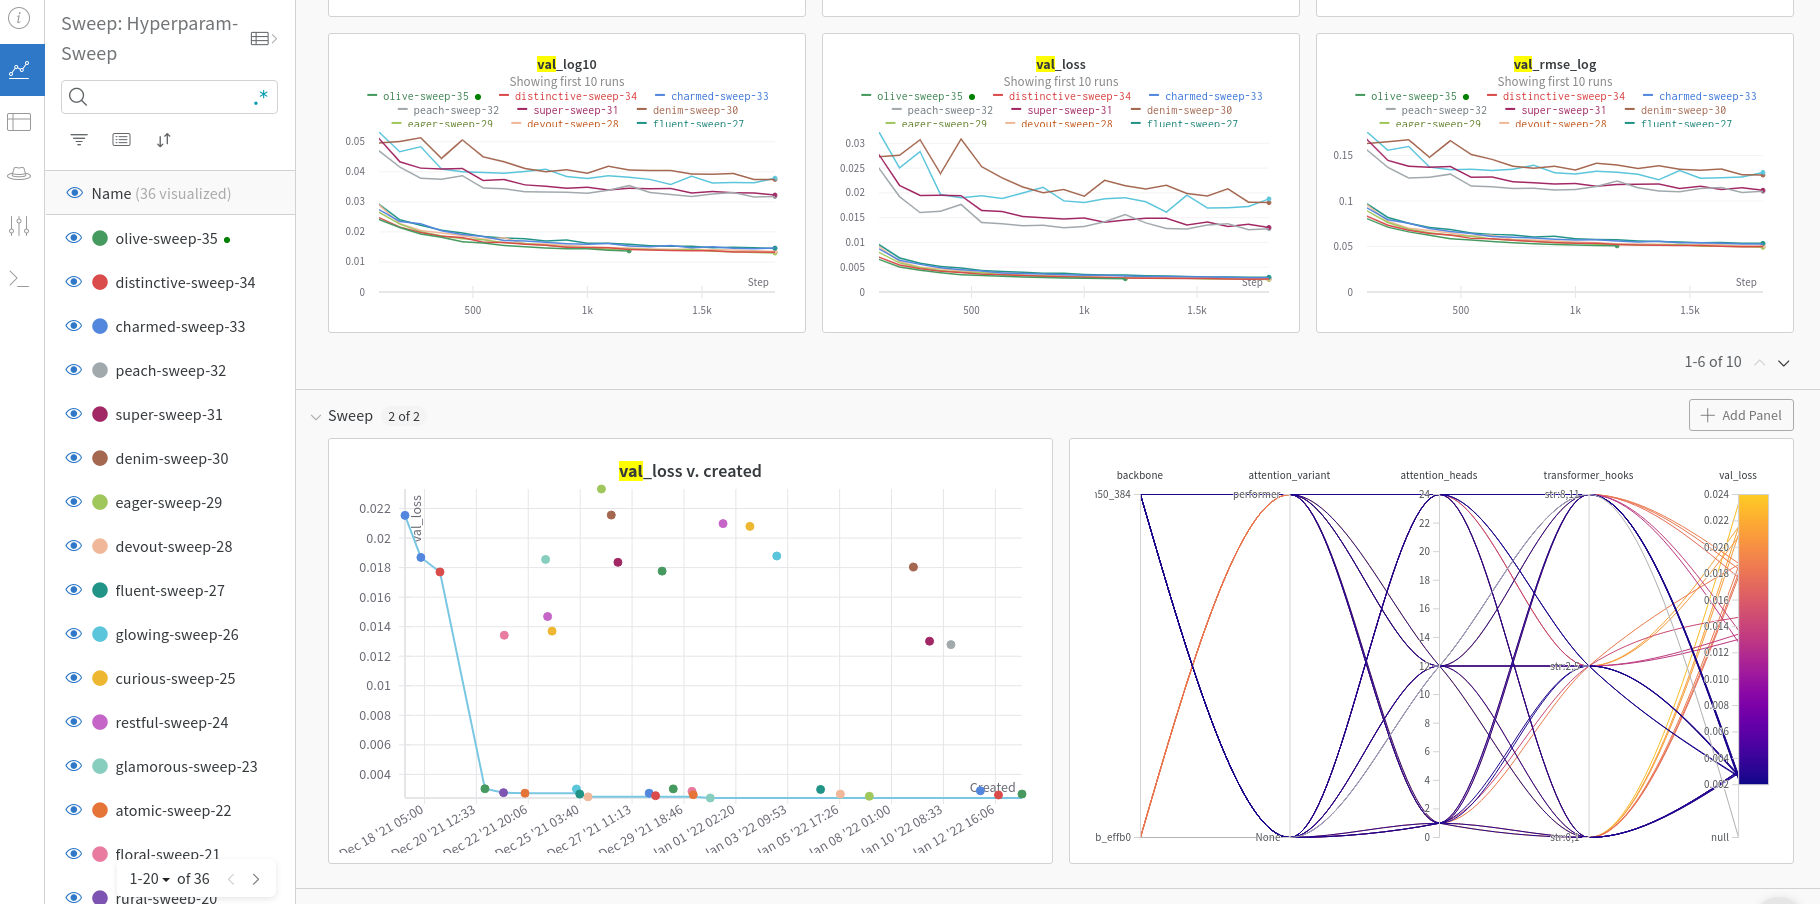
\includegraphics[width=\textwidth]{imagenes/wandb-ui.png}
\caption{Interfaz web de \textit{Weights and Biases}.}
\label{fig:wandb-ui}
\end{figure}

\textbf{Entorno de desarrollo}

Para gestionar la instalación y ejecución de este conjunto de \textit{software} en un entorno controlado, limitado, y fácilmente replicable, se ha elegido \textbf{Docker} junto al \textbf{NVIDIA Container Toolkit}. Docker proporciona una capa de abstracción virtualizando a nivel del sistema operativo. Esto significa que es capaz de utilizar el kernel de Linux de la máquina anfitrión, consiguiendo de esta forma ser mucho más rápido y eficiente que una máquina virtual. Por otro lado, el NVIDIA Container Toolkit envuelve el Docker Engine y mapea las primitivas de CUDA desde el interior del contenedor hasta el driver de la GPU del sistema anfitrión. De esta forma, la máquina anfitrión solo necesita tener actualizados los drivers de la(s) tarjeta gráfica para que puedan ser empleados de manera transparente por CUDA. Para el desarrollo, se parte de una de las imágenes proporcionadas por PyTorch con la versión de PyTorch y de CUDA necesarias donde se instalan todas las librerías requeridas. 

Si bien es cierto, existen otras opciones para conseguir entornos de desarrollo funcionalmente similares: Conda, por ejemplo, también gestiona las dependencias de CUDA de las librerías de aprendizaje profundo, pero puede entrar en conflicto con las librerías instaladas usando pip (el instalador de paquetes de Python) en su mismo entorno virtual, ya que no todas las librerías están disponibles en los repositorios de conda; otra opción que nos permite usar pip sin riesgo de dañar otras instalaciones en el equipo es el uso de entornos virtuales como venv, pero estos no gestionan correctamente el software y las dependencias de los paquetes relacionados con CUDA. 

No obstante, Docker ofrece una ventaja más que es decisiva, la portabilidad que ofrece entre sistemas. En caso de querer ejecutar los scripts en cloud (\ref{cloud}) o en dispositivos embebidos (p.e. los dispositivos Jetson de NVIDIA, que incluyen el NVIDIA Container Toolkit) sería suficiente con usar la misma imagen para tener un entorno idéntico. 

Los ficheros necesarios para crear el entorno empleado en el proyecto están disponibles tanto en el repositorio del proyecto como en el Anexo TODO.

% https://developer.nvidia.com/embedded/jetson-cloud-native
% https://github.com/NVIDIA/nvidia-docker/issues/1268

\textbf{Otros}

Por último, para la redacción de este documento se ha empleado \textbf{LaTeX} como sistema de composición de texto, \textbf{diagrams.net} para el diseño de figuras e ilustraciones, y \textbf{BibTeX} para gestionar las referencias bibliográficas. Tanto esta memoria como el desarrollo del código relacionado con el proyecto se han llevado a cabo empleado \textbf{Git} como software de control de versiones y se pueden encontrar en los repositorios TODO y TODO respectivamente.


\subsection{Hardware}
Para el desarrollo de este proyecto, se ha utilizado principalmente el Equipo 1 de la \Cref{tab:computer-specs}. No obstante, para el entrenamiento y la evaluación de los distintos modelos de aprendizaje profundo, se han empleado también instancias en la nube con la configuración del Equipo 2 en la \Cref{tab:computer-specs}.

\begin{table}[H]
\centering
\begin{tabular}{ccc}
\hline
\rowcolor[HTML]{FFFFFF} 
           & \begin{tabular}[c]{@{}c@{}}Equipo 1\\ (Sobremesa)\end{tabular}                   & \begin{tabular}[c]{@{}c@{}}Equipo 2\\ (Google Cloud)\end{tabular}      \\ \hline
\rowcolor[HTML]{EFEFEF} 
Procesador & \begin{tabular}[c]{@{}c@{}}AMD Ryzen 7 3800x \\ 8 núcleos @ 3.9 GHz\end{tabular} & \begin{tabular}[c]{@{}c@{}}Intel Xeon\\ 4 vCPU @ 2.30 GHz\end{tabular} \\
\rowcolor[HTML]{FFFFFF} 
GPU &
  \begin{tabular}[c]{@{}c@{}}NVIDIA RTX 3070 \\ 8 GB GDDR6\\ 5888 CUDA cores\\ 184 Tensor cores\\ Arquitectura Ampere\end{tabular} &
  \begin{tabular}[c]{@{}c@{}}NVIDIA Tesla T4\\ 16 GB GDDR6\\ 2560 CUDA cores\\ 320 Tensor cores\\ Arquitectura Turing\end{tabular} \\
\rowcolor[HTML]{EFEFEF} 
Memoria    & 32 GB DDR4                                                                       & 15 GB                                                                  \\ \hline
\end{tabular}
\caption{Especificaciones de los equipos empleados durante el trabajo de fin de máster.}
\label{tab:computer-specs}
\end{table}

\subsection{Datasets}
Durante este trabajo, de forma directa o indirecta, se emplean ciertos conjuntos de datos. Más concretamente, ImageNet \cite{imagenet_cvpr09, ILSVRC15} y MIX6 \cite{visiontransformersDPT} han sido empleados (no durante el desarrollo de este trabajo) para preentrenar los distintos modelos usados, mientras que KITTI \cite{KITTI-dataset, KITTI-benchmarks, KITTI-road-benchmark, KITTI-sceneflow-benchmark} se elige como conjunto de datos con el que comparar y evaluar las distintas modificaciones, implementadas y por lo tanto se utiliza para entrenar los modelos. A continuación se resumen las características de estos tres \textit{datasets}.

\subsubsection{ImageNet}
ImageNet \cite{imagenet_cvpr09, ILSVRC15} es un \textit{dataset} que proporciona un gran número de imágenes etiquetadas en función de la presencia o ausencia de una serie de conceptos definidos como \textit{synsets}. Estos conceptos siguen la jerarquía propuesta por WordNet \cite{wordnet}, donde se agrupan palabras y categorías en función de sus relaciones semánticas. Para construir ImageNet, partiendo de una fracción de la ya mencionada estructura de WordNet, se buscaron imágenes de Internet para poblar cada una de las categorías. Estas imágenes, se filtraron y posteriormente fueron manualmente etiquetadas por humanos. 

Dentro del proyecto de Imagenet, existen dos conjuntos: ImageNet21K e ImageNet1K (este último, normalmente llamado ImageNet). La principal diferencia entre estos dos conjuntos es que el primero, ImageNet21K suma más de 14 millones de imágenes clasificadas en más de 21 mil clases diferentes. Por otro lado, ImageNet1K es un subconjunto de ImageNet21K compuesto por cerca de 1.2 millones de imágenes clasificadas en 1000 categorías diferentes. Además de esto, también cuenta con anotaciones de localización de objetos (\textit{bounding boxes}) en más de medio millón de imágenes. Debido a la gran cantidad de imágenes y la variedad de elementos que abarcan, ImageNet es normalmente empleado para entrenar las arquitecturas de aprendizaje automático profundo. De esta forma, los modelos preentrenados en ImageNet pueden ajustarse de una manera mucho más rápida y efectiva a tareas e imágenes nuevas con otros \textit{datasets}, ya que al haber sido entrenados previamente los modelos han aprendido a extraer características generales (normalmente reutilizables) de las imágenes.

Una muestra de imágenes que conforman ImageNet está disponible en la \Cref{fig:imagenet}.
\begin{figure}[H]
\centering
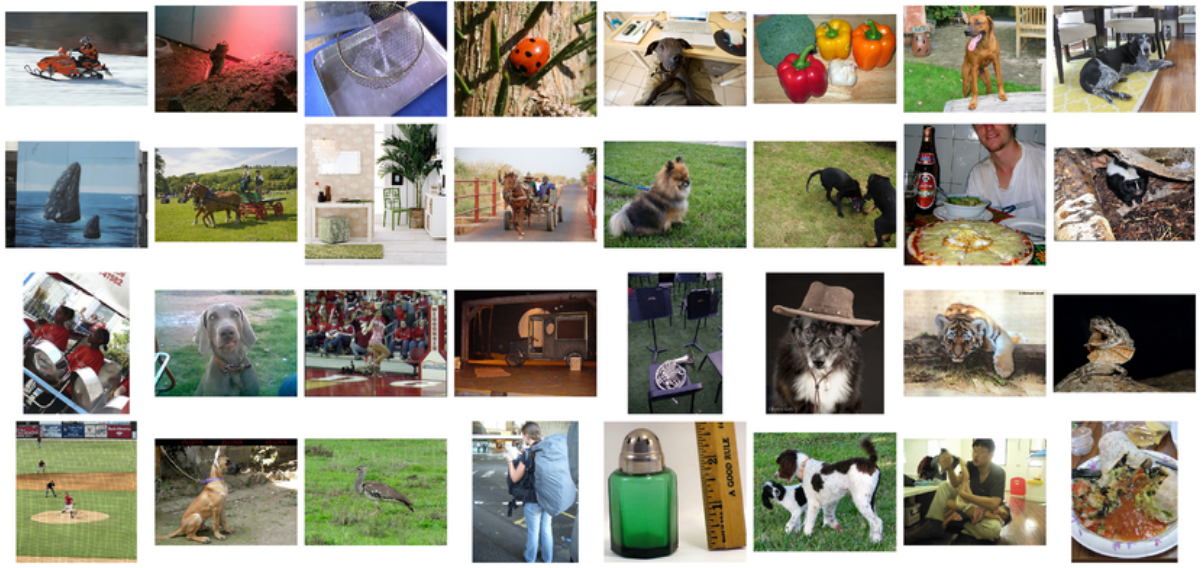
\includegraphics[width=\textwidth]{imagenes/imagenet.png}
\caption{Muestra de las imágenes de ImageNet. Fuente: \cite{ILSVRC15}}
\label{fig:imagenet}
\end{figure}

\subsubsection{MIX6}\label[seccion]{mix6}
%TODO Poner una nota al pie con los links de hacer los datasets piratas.
MIX6 \cite{visiontransformersDPT}, una ampliación de MIX5 \cite{midas-intel}, es en realidad una agrupación de otros \textit{datasets} que proporcionan anotaciones de profundidad de sus imágenes. Estas agrupaciones, consiguen dos características importantes: Primero, suman una cantidad de imágenes considerablemente alta; segundo, al tener datos de naturalezas tan distintas, existe una enorme variedad entre las imágenes, lo que permite entrenar modelos de estimación de profundidades generales, es decir, que no estén especializados en ningún entorno concreto. 

Estas dos características, hacen que MIX6 sea una muy buena opción para entrenar arquitecturas basadas en \textit{transformers} pero también dificultan el entrenamiento de modelos debido a la falta de homogeneidad entre los formatos de las imágenes, sus anotaciones, etc. Un desglose resumido de los \textit{datasets} que componen MIX6 está disponible en la \Cref{tab:mix6-datasets}.

% https://www.sascha-frank.com/Faq/tables_one.html
\begin{table}[H]
\centering
\resizebox{\textwidth}{!}{%
\begin{tabular}{@{}lcc@{}}
\toprule
\textit{Dataset}                                   & Descripción                                                                      & Núm. de imágenes \\ \midrule
Entrenamiento                                      & \multicolumn{1}{l}{}                                                             &                  \\ \midrule
\rowcolor[HTML]{EFEFEF} 
DIML Indoor \cite{DIML}                            & \cellcolor[HTML]{EFEFEF}Imágenes reales anotadas con cámara Kinect de Microsoft. & 220K             \\
MegaDepth \cite{MegaDepthLi18} &
  \begin{tabular}[c]{@{}c@{}}Imágenes reales anotadas con MVS \\ (\textit{Multi View Stereo} - Múltiples puntos de vista en diferentes fotografías)\end{tabular} &
  130K \\
\rowcolor[HTML]{EFEFEF} 
ReDWeb \cite{Xian_2018_CVPR}                       & Imágenes reales anotadas a partir de estereovisión.                              & 3.6K             \\
WSVD \cite{wang2019web} &
  \begin{tabular}[c]{@{}c@{}}Vídeos recuperados de YouTube en formato de estereovisión \\ anotados a partir de dicha pareja de imágenes.\end{tabular} &
  1.5M \\
\rowcolor[HTML]{EFEFEF} 
3D Movies \cite{midas-intel} &
  \begin{tabular}[c]{@{}c@{}}Películas 3D grabadas con cámaras estereoscópicas \\ anotadas a partir de la pareja de imágenes.\end{tabular} &
  75K \\
\underline{TartanAir} \cite{tartanair2020iros}     & Imágenes sínteticas.                                                             & 1M               \\
\rowcolor[HTML]{EFEFEF} 
\underline{HRWSI} \cite{Xian_2020_CVPR} &
  \cellcolor[HTML]{EFEFEF}Imágenes reales anotadas a partir de estereovisión. &
  21K \\
\underline{ApolloScape} \cite{wang2019apolloscape} & Imágenes reales anotadas con sensor LiDAR.                                       & 5.1K             \\
\rowcolor[HTML]{EFEFEF} 
\underline{BlendedMVS} \cite{blendedMVS}           & Imágenes sínteticas.                                                             & 17K              \\
\underline{IRS} \cite{IRS}                         & \cellcolor[HTML]{FFFFFF}Imágenes sínteticas.                                     & 103K             \\ \midrule
Evaluación                                         & \multicolumn{1}{l}{}                                                             &                  \\ \midrule
\rowcolor[HTML]{EFEFEF} 
DIW \cite{DIW} &
  \begin{tabular}[c]{@{}c@{}}Imágenes reales anotadas manualmente con la profundidad \\ relativa entre pares de puntos aleatorios.\end{tabular} &
  495K \\
ETH3D \cite{schoeps2017cvpr}                       & Imágenes reales anotadas con sensor LiDAR.                                       & 5.2K             \\
\rowcolor[HTML]{EFEFEF} 
Sintel \cite{Butler:ECCV:2012}                     & Imágenes sintéticas.                                                             & 1K               \\
KITTI \cite{KITTI-dataset}                         & Imágenes reales anotadas con sensor LiDAR.                                       & 45K              \\
\rowcolor[HTML]{EFEFEF} 
NYUDepthV2 \cite{nyudepthv2}                       & Imágenes reales anotadas con cámara Kinect de Microsoft.                         & 407K             \\
TUM \cite{sturm12iros}                             & \cellcolor[HTML]{FFFFFF}Imágenes reales anotadas con cámara Kinect de Microsoft. & 87K              \\ \bottomrule
\end{tabular}%
}
\caption{Datasets que conforman MIX6. Subrayados aquellos que no forman parte de MIX5.}
\label{tab:mix6-datasets}
\end{table}

\todo{Esta tabla no me convence mucho pero tampoco se me ocurre como resumirlo mejor}

\subsubsection{KITTI}
KITTI \cite{KITTI-dataset, KITTI-benchmarks, KITTI-road-benchmark, KITTI-sceneflow-benchmark} es un proyecto desarrollado por el \textit{Karlsruhe Institute of Technology} y el \textit{Toyota Technological Institute} que engloba un \textit{dataset} y un conjunto de \textit{becnhmarks} enfocados a diferentes tareas relacionadas con la conducción autónoma. Los \textit{benchamrks} que incluye este proyecto evalúan: estereovisión, flujo óptico (\textit{optical flow}), flujo de la escena, \textbf{estimación de profundidades monocular}, \textit{depth completion}, odometría visual/SLAM, localización de objetos (2D, 3D y cenital), seguimiento de objetos, segmentación de carreteras, y por último, segmentación de objetos general, tanto semántica como a nivel de instancia. Debido a la naturaleza de este trabajo, este apartado se centrará en la parte referente a la predicción de profundidad monocular.

\begin{table}[H]
\centering
\begin{tabular}{@{}lcr@{}}
\toprule
Tipo de sensor       & Modelo                & Características                                                                                               \\ \midrule
\rowcolor[HTML]{EFEFEF} 
Cámara escala de grises (x2) & PointGray Flea2 grayscale & \begin{tabular}[c]{@{}r@{}}Sensor: FL2-14S3M 1.4 MP\\ 1/2” Sony ICX267 CCD\\ Global Shutter\end{tabular} \\
Cámara color (x2)    & PointGray Flea2 color & \begin{tabular}[c]{@{}r@{}}Sensor: FL2-14S3M 1.4 MP\\ 1/2” Sony ICX267 CCD\\ Global Shutter\end{tabular}      \\
\rowcolor[HTML]{EFEFEF} 
Escáner láser (x1)   & Velodyne HDL-64E      & \begin{tabular}[c]{@{}r@{}}64 haces a $10 Hz$\\ Resolución en distancia: $2 cm$\\ Rango: $120 m$\end{tabular} \\
Medida inercial (x1) & OXTS RT3003           & \begin{tabular}[c]{@{}r@{}}Posicionamiento GPS\\ Velocímetro\\ Acelerómetro - Giroscopio\end{tabular}         \\ \bottomrule
\end{tabular}
\caption{Sensores equipados en el vehículo empleado para recoger los datos de KITTI.}
\label{tab:sensores-kitti}
\end{table}

\todo{Esta tabla puede que sea un poco demasiado}

Los datos disponibles en KITTI fueron capturados empleando un vehículo equipado con diferentes sensores (\Cref{tab:sensores-kitti}) para realizar diferentes recorridos en distintas zonas urbanas e interurbanas. De esta forma, se capturaron escenarios variados en múltiples condiciones de luz, hora, presencia de vehículos y peatones, etc. Dentro de los sensores equipados, son de especial interés para este trabajo las dos parejas de cámaras para estereovisón (un montaje con dos cámaras en escala de grises y otro montaje con dos cámaras en color) y el escáner láser rotatorio de $360\degree$. Además de estos sensores, el automóvil también equipaba un sensor de medida inercial con sistema de navegación GPS para registrar información relacionada con la odometría que no se ha empleado durante el desarrollo del trabajo.

% (\textit{2x PointGray Flea2 grayscale cameras, FL2-14S3M-C, 1.4 Megapixels, 1/2” Sony ICX267 CCD, global shutter}) 
 
% (\textit{2x PointGray Flea2 color cameras (FL2-14S3M-C), 1.4 Megapixels, 1/2” Sony ICX267 CCD, global shutter}) - 
 
% \textit{Velodyne HDL-64E rotating 3D laser scanner, 10 Hz, 64 beams, 0.09 degree angular resolution, 2 cm distance accuracy, collecting $\sim$ 1.3 million points/second, field of view: $360\degree$ horizontal, $26.8\degree$ vertical, range: 120 m}. 

\paragraph{Datos}\mbox{}\\
Si nos centramos en la información relevante para la estimación de profundidades monocular, KITTI ofrece los siguientes datos:

\textbf{Datos en bruto}

El \textit{dataset} está compuesto por fotogramas muestreados y sincronizados a 10 Hz de los vídeos capturados por las cámaras en diferentes recorridos. Debido a las características del sistema óptico, para cada instante se disponen de cuatro imágenes, derecha e izquierda en escala de grises, y derecha e izquierda en color. Una muestra de estas imágenes puede observarse en la \Cref{fig:kitti-raw}.

\begin{figure}[H]
\centering
	\subfloat[Imagen en escala de grises capturada por la cámara izquierda.]{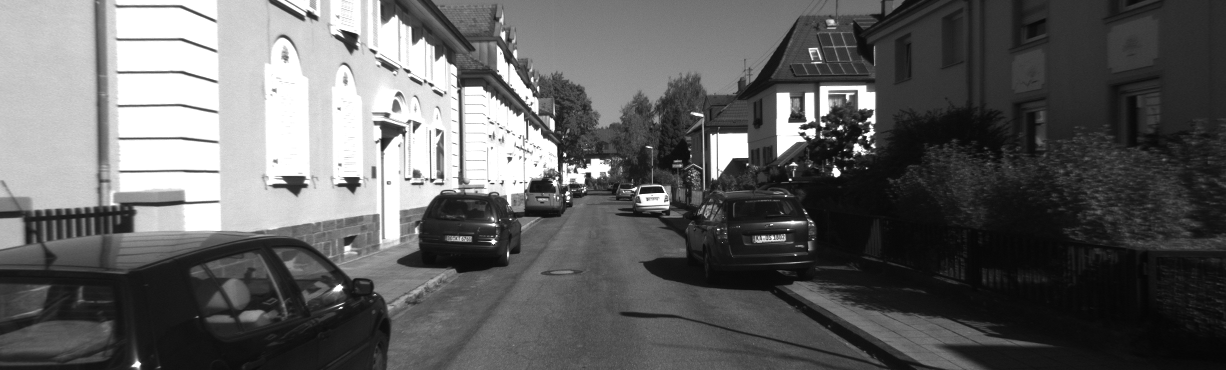
\includegraphics[width=0.48\textwidth]{imagenes/67_img0.png} } 
\hfil
	\subfloat[Imagen en escala de grises capturada por la cámara derecha.]{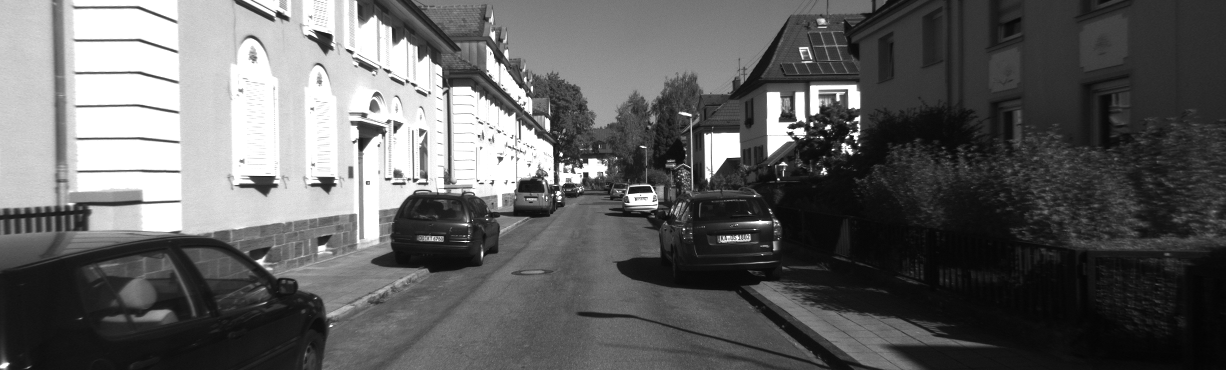
\includegraphics[width=0.48\textwidth]{imagenes/67_img1.png} }\\[-2ex]

	\subfloat[Imagen en color capturada por la cámara izquierda.]{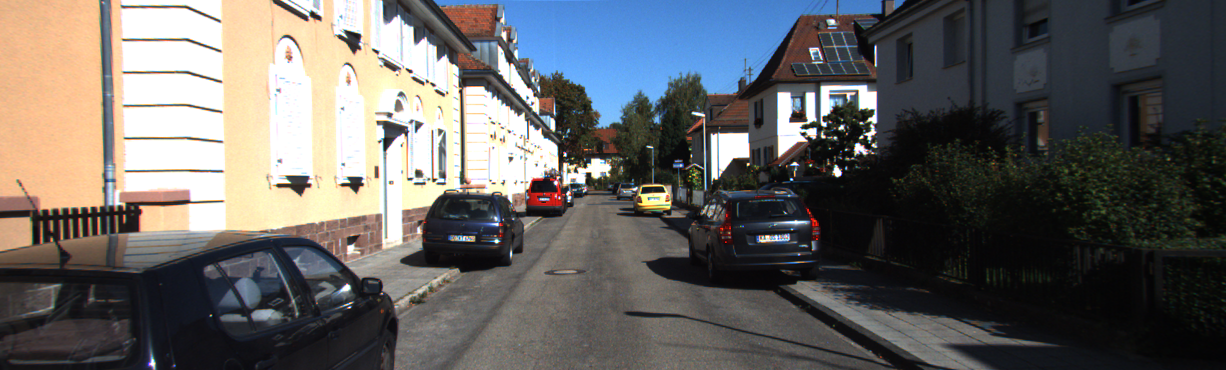
\includegraphics[width=0.48\textwidth]{imagenes/67_img2.png}} 
\hfil
	\subfloat[Imagen en color capturada por la cámara derecha.]{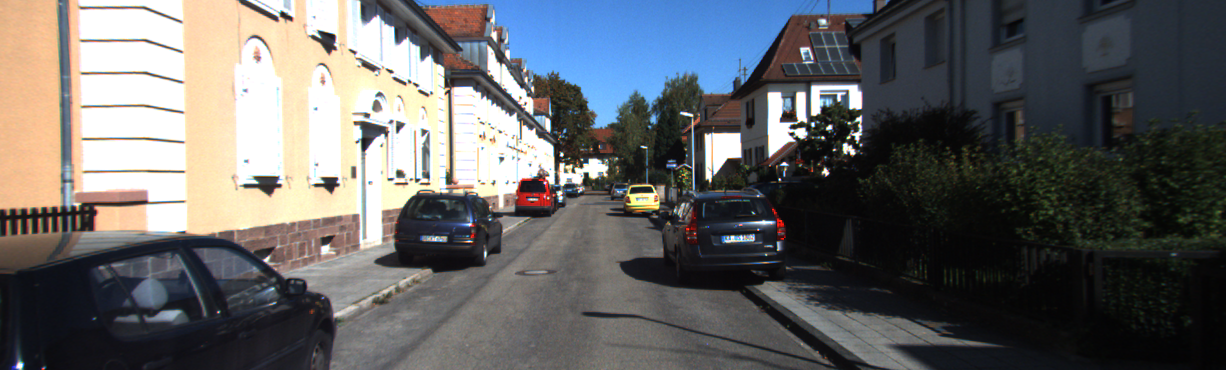
\includegraphics[width=0.48\textwidth]{imagenes/67_img3.png}}\\[-2ex]
	
\caption{Muestra de las cuatro imágenes en bruto disponibles en KITTI para un instante dado.}
\label{fig:kitti-raw}
\end{figure}

En total, se disponen de 192760 imágenes ($\sim$ 196 GB) de tamaño 1242x375 píxeles, de las cuales 96430 (la mitad) corresponden a las cámaras a color. Como el objetivo es la estimación de profundidades monocular, solo se emplea una de las imágenes de cada pareja de imágenes producido por el sistema de estereovisión, por lo que realmente se emplean 48215 imágenes de los datos en bruto (una cuarta parte de la cantidad original).

% Son metros * 256, es decir, un píxel que vale 640 en la imágen son 640/256=2.5 metros. 
\textbf{Anotaciones}

Por otro lado, KITTI proporciona también los valores numéricos de la profundidad para cada uno de los píxeles (de las imágenes presentadas previamente) almacenados como imágenes en formato PNG con un solo canal y 16 bits para cada valor (UINT16). Estos valores son los obtenidos por el escaner láser equipado en el vehículo y pueden considerarse una medida fiable de la profundidad en cada imagen. Por lo tanto serán los datos que se emplearan como anotaciones para entrenar los modelos y evaluar sus capacidades de estimación de profundidades. Un punto importante a considerar sobre las medidas de estas anotaciones es que debido a la naturaleza del sensor con el que fueron tomadas, son anotaciones \textbf{dispersas} (\textit{sparse}), no densas. Esto significa que no todos los píxeles de una imagen tienen anotación, y por lo tanto aquellos píxeles no anotados deberán ser ignorados tanto durante el entrenamiento como durante la evaluación. Una muestra de estas etiquetas y de las anotaciones dispersas puede observarse en la \Cref{fig:kitti_depth}. Estas anotaciones están disponibles tanto como para las imágenes capturadas con las cámaras derechas como para las capturadas con las cámaras izquierdas.

\begin{figure}[H]
\centering
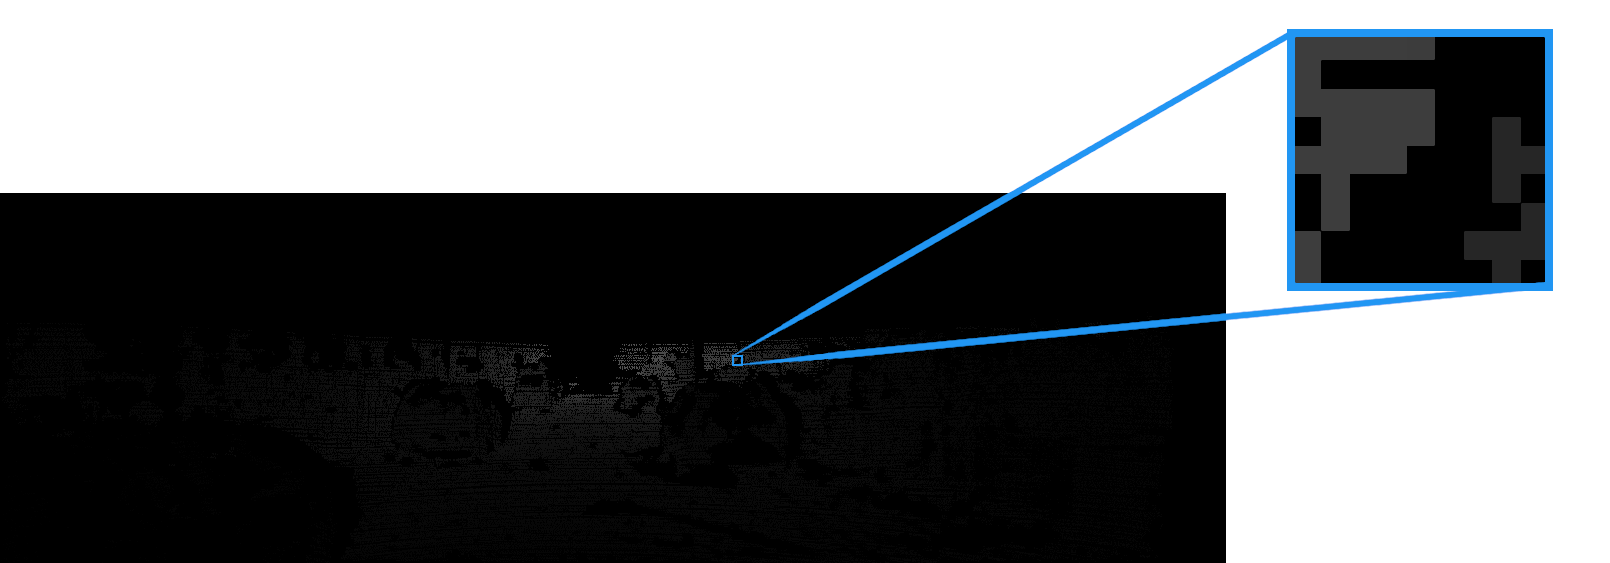
\includegraphics[width=\textwidth]{imagenes/depth67_img3_detail.png}
\caption{Anotación de KITTI y detalle de su carácter disperso para un instante dado.}
\label{fig:kitti_depth}

\end{figure}

\paragraph{Conjuntos de entrenamiento, validación y evaluación}\label[seccion]{conjuntos-kitti}\mbox{}\\
Para el desarrollo de este trabajo es necesario disponer de un conjunto de entrenamiento con el que ajustar los parámetros de los modelos, un conjunto de validación con el que comprobar que no se está sobre ajustando el modelo al primer conjunto y para elegir la combinación de hiperparámetros óptima, y por último, un conjunto de evaluación (\textit{test}) en el que calcular una serie de métricas que nos aportarán información del rendimiento real de los modelos finales.

El \textit{dataset} de KITTI ya está dividido en entrenamiento y validación, e incluye una descarga adicional con el conjunto de test para el cual no están disponibles públicamente las anotaciones. No obstante, en las publicaciones sobre estimación de profundidad monocular \cite{visiontransformersDPT, monodepth,midas-intel, bts} es común encontrar los conjuntos de entrenamiento, validación y evaluación definidos por Eigen et al. \cite{eigen-multi-scale} (conocidos como el \textit{Eigen split}) que no respetan las particiones originales del \textit{dataset} de KITTI. 

Las listas con los archivos que pertenecen a cada uno de las particiones se han descargado desde el repositorio\footnote{\url{https://github.com/nianticlabs/monodepth2/tree/master/splits} - (\textit{Eigen full})} del trabajo de Godard et al. \cite{monodepth}. En estas listas, hay nombres de archivos que no tienen ninguna anotación asociada, por lo que se eliminan de sus respectivas particiones. La distribución del número de imágenes, así como el número de imágenes eliminadas de cada conjunto se muestran en la \Cref{tab:kitti-splits}.

\todo{Adjuntar el código usado para estas cosillas?}

\begin{table}[H]
\centering
\begin{tabular}{@{}cccc@{}}
\toprule
\multicolumn{1}{l}{}       & \multicolumn{1}{l}{} & \multicolumn{1}{l}{Eigen split} & \multicolumn{1}{l}{} \\ \cmidrule(l){2-4} 
\rowcolor[HTML]{FFFFFF} 
                        & Entrenamiento & Validación & Evaluación \\ \midrule
\rowcolor[HTML]{EFEFEF} 
Num. de archivos        & 45200         & 1776       & 697        \\
\rowcolor[HTML]{FFFFFF} 
Imágenes no encontradas & 0 (0\%)       & 0 (0\%)    & 0 (0\%)    \\
\rowcolor[HTML]{EFEFEF} 
Anotaciones no encontradas & 630 (1.39\%)         & 30 (1.69\%)                     & 45 (6.46\%)          \\
\rowcolor[HTML]{FFFFFF} 
Num. imágenes útiles    & 44570         & 1746       & 652        \\ \bottomrule
\end{tabular}
\caption{Distribución de las imágenes y número de imágenes no encontradas en el dataset.}
\label{tab:kitti-splits}
\end{table}

Como comprobación adicional, se han cruzado las listas de archivos descargadas para asegurar que ninguno de los elementos de los conjuntos de entrenamiento y validación se encuentras en el conjunto de evaluación.


\subsection{Definición de modelos a entrenar}
Uno de los objetivos de este Trabajo Fin de Máster es explorar distintas modificaciones en la arquitectura DPT \cite{visiontransformersDPT}. Para poder comparar de forma exhaustiva los efectos y la influencia en el rendimiento de cada una de estas modificaciones, se exploran todas las combinaciones posibles de los valores que se van a estudiar. Por lo tanto, no se detiene el entrenamiento de ningún modelo en caso de que su rendimiento sea peor que los modelos ya entrenados, ni se optimiza la búsqueda en función de la influencia de cada modificación en una métrica concreta.

Para definir tantos modelos como combinaciones sean posibles, se toman los conjuntos de valores elegidos para cada una de las modificaciones planteadas y se calcula su producto cartesiano (\textit{grid search}). De esta forma, se obtienen las arquitecturas de los modelos que se entrenarán durante este trabajo y de los que se obtendrán los resultados finales.


\subsection{Evaluación}
Para la evaluación de los modelos presentados en este trabajo y sus modificaciones, se ha seguido la metodología propuesta en la publicación de Lee et al. \cite{bts} para evaluar los resultados en KITTI que consiste en recortar un pequeño marco alrededor de la imagen de salida y crear una máscara para los píxeles que no tienen una profundidad definida en la anotación. En la publicación de DPT \cite{visiontransformersDPT}, también se emplea el mismo procedimiento.

Al usar esta misma metodología se satisfacen dos objetivos: poder reproducir los resultados presentados en dicho artículo con el modelo original, y evaluar las modificaciones introducidas para comparar sus resultados con los del modelo sin modificar. 

Como se mencionará más adelante, una de las modificaciones introducidas en este trabajo reduce el tamaño de la imagen en la entrada de las arquitecturas. El resultado de estos modelos, no obstante, se escala a su tamaño original antes de llevar a cabo la evaluación para asegurar que la magnitud de las métricas se ajuste a la del modelo original (con entradas de mayor resolución).

\subsubsection{Métricas}
Una vez escaladas y enmascaradas las predicciones y las anotaciones, se calculan una serie de valores cuantitativos que permiten comparar y evaluar el rendimiento de los modelos. Las funciones que nos proporcionan estos valores son conocidas como métricas. Dentro del gran número de funciones que permiten evaluar los resultados de los modelos, se han elegido aquellas comúnmente empleadas en los modelos de aprendizaje profundo dedicados a la estimación de profundidad en imágenes monoculares \cite{visiontransformersDPT,bhat2020adabins,eigen-multi-scale,midas-intel,bts,DORN,evaluation-cnn-depth-estimation, depth-estimation-metrics}.

En las siguientes ecuaciones, $d_p$ representa el valor del mapa de profundidad original (anotación) para cada pixel $p$, mientras que $\hat{d}_p$ representa el valor de la profundidad estimada por el modelo para cada pixel $p$. Por otro lado, $T$ denota el número de píxeles con información de profundidad disponibles en la anotación (al ser anotaciones dispersas, las imágenes no tienen información sobre la profundidad en todos los píxeles).


\paragraph{\textit{Accuracy under a threshold}}\mbox{}\\
La primera de estas métricas, el \textit{accuracy under a threshold}, viene dada por la \Cref{eqn:accuracy_under_thr} y cuantifica el porcentaje de píxeles a los que el modelo ha asignado una profundidad cuya relación de escala respecto de su valor real es menor que un determinado umbral. Los valores que se emplean para este umbral son $1.25$, $1.25^2$ y $1.25^3$.

\begin{equation}
\label{eqn:accuracy_under_thr}
\% \ de \ p \in T : max(\frac{\hat{d}_p}{d_p},\frac{d_p}{\hat{d_p}}) = \delta < umbral 
\end{equation}

\paragraph{\textit{Mean Absolute Value of the Relative Error (Abs Rel)}}\mbox{}\\
Otra métrica usada habitualmente es el promedio del error relativo en todos los píxeles que disponen de valor de profundidad anotada. Para conseguir este error relativo, se calcula el error absoluto y se divide entre el valor real de la profundidad (\Cref{eqn:abs_rel}).

% np.mean(np.abs(gt - pred) / gt)
\begin{equation}
\label{eqn:abs_rel}
\frac{1}{T}\sum_{p\ \in\ T} \frac{|d_p - \hat{d}_p|}{d_p}
\end{equation}

\paragraph{\textit{Mean Squared Relative Error (Sq Rel)}}\mbox{}\\
Similar a la métrica anterior, en este caso el error absoluto se eleva al cuadrado antes de ser dividido entre el valor a estimar y de promediarlo con el resto de píxeles (\Cref{eqn:sq_rel}). De esta forma, por la naturaleza cuadrática de la fórmula, se le da una mayor importancia a los errores mayores que a los menores.

% np.mean(((gt - pred)**2) / gt)
\begin{equation}
\label{eqn:sq_rel}
\frac{1}{T}\sum_{p\ \in\ T} \frac{(d_p - \hat{d}_p)^2}{d_p}
\end{equation}

\paragraph{\textit{Linear Root Mean Squared Error (RMSE)}}\mbox{}\\
El valor del error cuadrático medio proporciona una medida del promedio de la magnitud de la diferencia entre la profundidad predicha para cada uno de los píxeles y su profundidad real (\Cref{eqn:rmse}). Una característica interesante de esta métrica es que sus unidades coinciden con las de la variable predicha, lo que facilita su interpretación. Como los errores se elevan al cuadrado antes de promediarse, estos tienen una importancia relativa directamente relacionada con su magnitud, es decir, cuanto mayor sea el error, más peso tendrá en el promedio. Es por esto por lo que es especialmente útil si se busca penalizar más los errores más grandes en las predicciones.

\begin{equation}
\label{eqn:rmse}
\sqrt{\frac{1}{T}\sum_{p\ \in\ T} (d_p - \hat{d}_p)^2}
\end{equation}

\paragraph{\textit{Logarithmic Root Mean Squared Error (RMSElog)}}\mbox{}\\
Similar a la métrica anterior, en este caso el error cuadrático medio se calcula sobre los logaritmos naturales de las medidas a comparar (\Cref{eqn:rmselog}). Al realizar la resta de los logaritmos, la operación es equivalente a calcular el logaritmo de la división del valor de profundidad estimado y el valor de profundidad anotado, restando de esta forma importancia a la escala del error y obteniendo una aproximación al error relativo de las medidas (frente al \textit{RMSE}, que sería una medida del error absoluto). Además, debido al escalado que realizan los logaritmos, los \textit{outliers} pierden importancia, por lo que es una métrica más robusta frente a este tipo de errores puntuales.

Otra característica a destacar de esta métrica es que está sesgada para penalizar aquellos casos en los que el valor predicho es menor que el valor real (subestimación). De esta forma, el error en dicha situación será mayor que si el valor predicho es mayor que el valor real (sobreestimación) aún cuando la diferencia entre ambos valores sea la misma.

%RMSElog es una medida del error relativo, RMSE es una medida del error absoluto
\begin{equation}
\label{eqn:rmselog}
\sqrt{\frac{1}{T}\sum_{p\ \in\ T} (\ln{d_p} - \ln{\hat{d}_p})^2}
\end{equation}

\paragraph{\textit{Scale Invariant Logarithmic Error (SIlog)}}\mbox{}\\
Esta métrica, es la raíz cuadrada de la función de pérdida propuesta por Eigen et al. \cite{eigen-multi-scale} con $\lambda = 1$ (\Cref{eqn:silog}). Al fijar el valor de $\lambda$ en la unidad, se obtiene una medida totalmente independiente de la escala de la salida. De esta forma, se obtiene una medida de la calidad de los resultados de los modelos ignorando completamente la escala en la que se han producido las predicciones, que como ya se ha comentado es uno de los problemas fundamentales de la estimación de profundidades en imagen monocular.

\todo[inline]{Aquí no sé que hacer, he hecho la demostración matemática de que es invariante a la escala pero es un churro de ecuaciones, no sé si merece la pena poner un anexo solo para eso. La función de pérdida es esta misma así que más abajo cuando hablo de ella vuelvo a tener el mismo dilema}

% np.sqrt(np.mean((np.log(pred) - np.log(gt)) ** 2) - np.mean(np.log(pred) - np.log(gt)) ** 2) * 100
\begin{equation}
\label{eqn:silog}
\sqrt{
	\frac{1}{T} \sum_{p\ \in\ T} (\ln{d_p} - \ln{\hat{d_p}})^2
	-
	{\left(\frac{1}{T} \sum_{p\ \in\ T} \ln{d_p} - \ln{\hat{d_p}}\right)}^2
} * 100
\end{equation}

\paragraph{\textit{Mean Logarithmic Error (Log10)}}\mbox{}\\
Por último, se calculará también el promedio del error (en escala logarítmica) de las profundidades predichas respecto de las profundidades reales siguiendo la \Cref{eqn:log10}.

% np.mean(np.abs(np.log10(pred) - np.log10(gt)))
\begin{equation}
\label{eqn:log10}
\frac{1}{T} \sum_{p\ \in\ T} |\log_{10}{d_p} - \log_{10}{\hat{d}_p}|
\end{equation}

\paragraph{Velocidad de procesamiento}\mbox{}\\
Además de la calidad de los resultados, es de especial interés en este trabajo obtener medidas relacionadas con la velocidad de procesamiento que pueden alcanzar los modelos. Dentro de las medidas empleadas hay dos grupos: condicionadas por el \textit{hardware} utilizado (Tiempo de inferencia y Tasa de transferencia efectiva) e independientes del \textit{hardware} (Número de operaciones en coma flotante).

\subparagraph{Tiempo de inferencia}\mbox{}\\
Esta medida corresponderá al tiempo que tarda el modelo en procesar \textbf{una sola} imagen. Si suponemos que la aplicación de estos modelos es el procesamiento de vídeo de forma online, donde los fotogramas no pueden procesarse en lotes, esta medida es la inversa de los fotogramas por segundo (\textit{FPS}). 
Como se ha mencionado antes, esta métrica estará sujeta al \textit{hardware} en el que se ejecute, y por lo tanto variará de un equipo a otro.

\subparagraph{Tasa de transferencia efectiva \textit{(Throughput)}}\mbox{}\\
Por otro lado, en caso de que el procesamiento de imágenes se haga de forma offline y se disponga de todas las imágenes antes de comenzar el procesamiento, estas se podrían agrupar en lotes (\textit{batches}) para paralelizar su inferencia. Al paralelizar el procesamiento de las entradas, aumenta el número de imágenes que se puede procesar por unidad de tiempo, que es lo que medirá esta métrica. Es decir, la tasa de transferencia efectiva es el número máximo de imágenes que puede procesar un modelo por unidad de tiempo.
De nuevo, como se ha mencionado en el párrafo introductorio, este valor está ligado al equipo en el que se lleve a cabo la inferencia.

\subparagraph{Número de operaciones en coma flotante \textit{(FLOPs)}}\mbox{}\\
Por último, esta vez independiente del \textit{hardware} en el que se ejecuta el modelo, se empleará el número de operaciones en coma flotante (en inglés, FLOPs) que se requieren para procesar una sola entrada de la red como medida de la complejidad y coste computacional de los modelos.

% \todo[inline]{Si quantizamos los modelos a int8 dejamos de tener operaciones en coma flotante y esta métrica no servirá de nada. Explorar la opción de usar MACs (\url{https://en.wikipedia.org/wiki/Multiply\%E2\%80\%93accumulate_operation}). En el paper de FastDepth es lo que hacen.}

%% Mencionar que las pruebas se llevaran a cabo en distintos entornos y que esto se señalará en los resultados.

% \subsection{Portabilidad (?) de los modelos}
% Explicar el proceso que se ha llevado a cabo con onnx y por qué se emplea, explicar que hace onnx por debajo, hacer diagramas. Puede que esto colapse con la sección de software de arriba, se puede quitar.


\clearpage

\section{Desarrollo y modificaciones de la arquitectura}

En este capítulo, se introducen los cambios y desarrollos principales que se han llevado a cabo durante el trabajo.

\subsection{Cloud} 

Con el objetivo de reducir el tiempo necesario para entrenar los distintos modelos que se plantean en este trabajo, se ha recurrido al servicio de infraestructura (IaaS - \textit{Infraestructure as a Service}) que ofrece la empresa Google: Google Cloud. Los servicios en la nube (\textit{cloud}), permiten disponer de recursos informáticos de manera flexible, pagando únicamente por aquellos que estén activos. Los proveedores de IaaS, se encargan del mantenimiento y gestión de la infraestructura (redes, almacenamiento, servidores, virtualización), mientras que el usuario se encarga de la gestión del sistema operativo y todo lo que hay por encima. 

Dentro de Google Cloud, se han empleado los servicios \textbfit{Compute Engine}, para disponer de máquinas virtuales y \textbfit{Cloud Storage}, para crear recursos de almacenamiento (\textit{buckets}).

El flujo de trabajo que se ha seguido ha sido el siguiente (\ref{fig:cloud-diagram}):

\begin{enumerate}
\item Primero, se ha creado un \textit{bucket} en el que se han dejado disponibles el conjunto de datos empleado durante el entrenamiento, el código necesario para ejecutar el entrenamiento, y una serie de scripts para facilitar la configuración del equipo. Al disponer de estos archivos en la nube, se desacoplan totalmente la configuración de las máquinas virtuales y el ordenador local en el que se lleva a cabo el desarrollo (Equipo 1 en Tabla \ref{tab:computer-specs}).
\item A continuación, se configura una máquina virtual con el \textit{hardware} elegido\footnote{Para elegir el \textit{hardware} de las máquinas virtuales, se ha elegido la GPU que mayor relación TFLOPS/euro ofrecía para minimizar el coste de los equipos. El resto de características se han elegido de forma que la limitación del equipo sea el procesamiento en GPU.} (Equipo 2 en Tabla \ref{tab:computer-specs}). Una vez conectados a esta máquina virtual a través de SSH, se descarga del \textit{bucket} creado el script de configuración (disponible en el Anexo TODO) y se ejecuta. Este script, se encarga de: descargar el resto de archivos disponibles en el \textit{bucket}, instalar los drivers de NVIDIA necesarios para poder usar la GPU de la instancia, instalar Docker y el NVIDIA Container Toolkit, instalar Weights and Biases, y construir la imagen de Docker especificada en el Dockerfile descargado.
\item Una vez configurada la instancia con todos los archivos necesarios en su disco SSD, se crea una imagen de dicha instancia en Google Cloud de forma que sea fácilmente replicable. Posteriormente, se configura desde la consola de Google Cloud el inicio de estas instancias de forma que cada vez que se encienda una (nueva o ya existente), se cree dentro del equipo un contenedor de Docker a partir de la imagen ya construida, y se ejecute en este contenedor el cliente de Weight and Biases para entrenar modelos automáticamente. De esta forma, para añadir una nueva máquina al proceso de entrenamiento de experimentos, solamente hay que crear un nuevo equipo a partir de la imagen preconfigurada.
\item Por último, una vez finalizados los experimentos, se copia a través de SSH los parámetros de los modelos entrenados, que se han guardado en cada una de las máquinas virtuales empleadas.
\end{enumerate}

\begin{figure}[H]
\centering
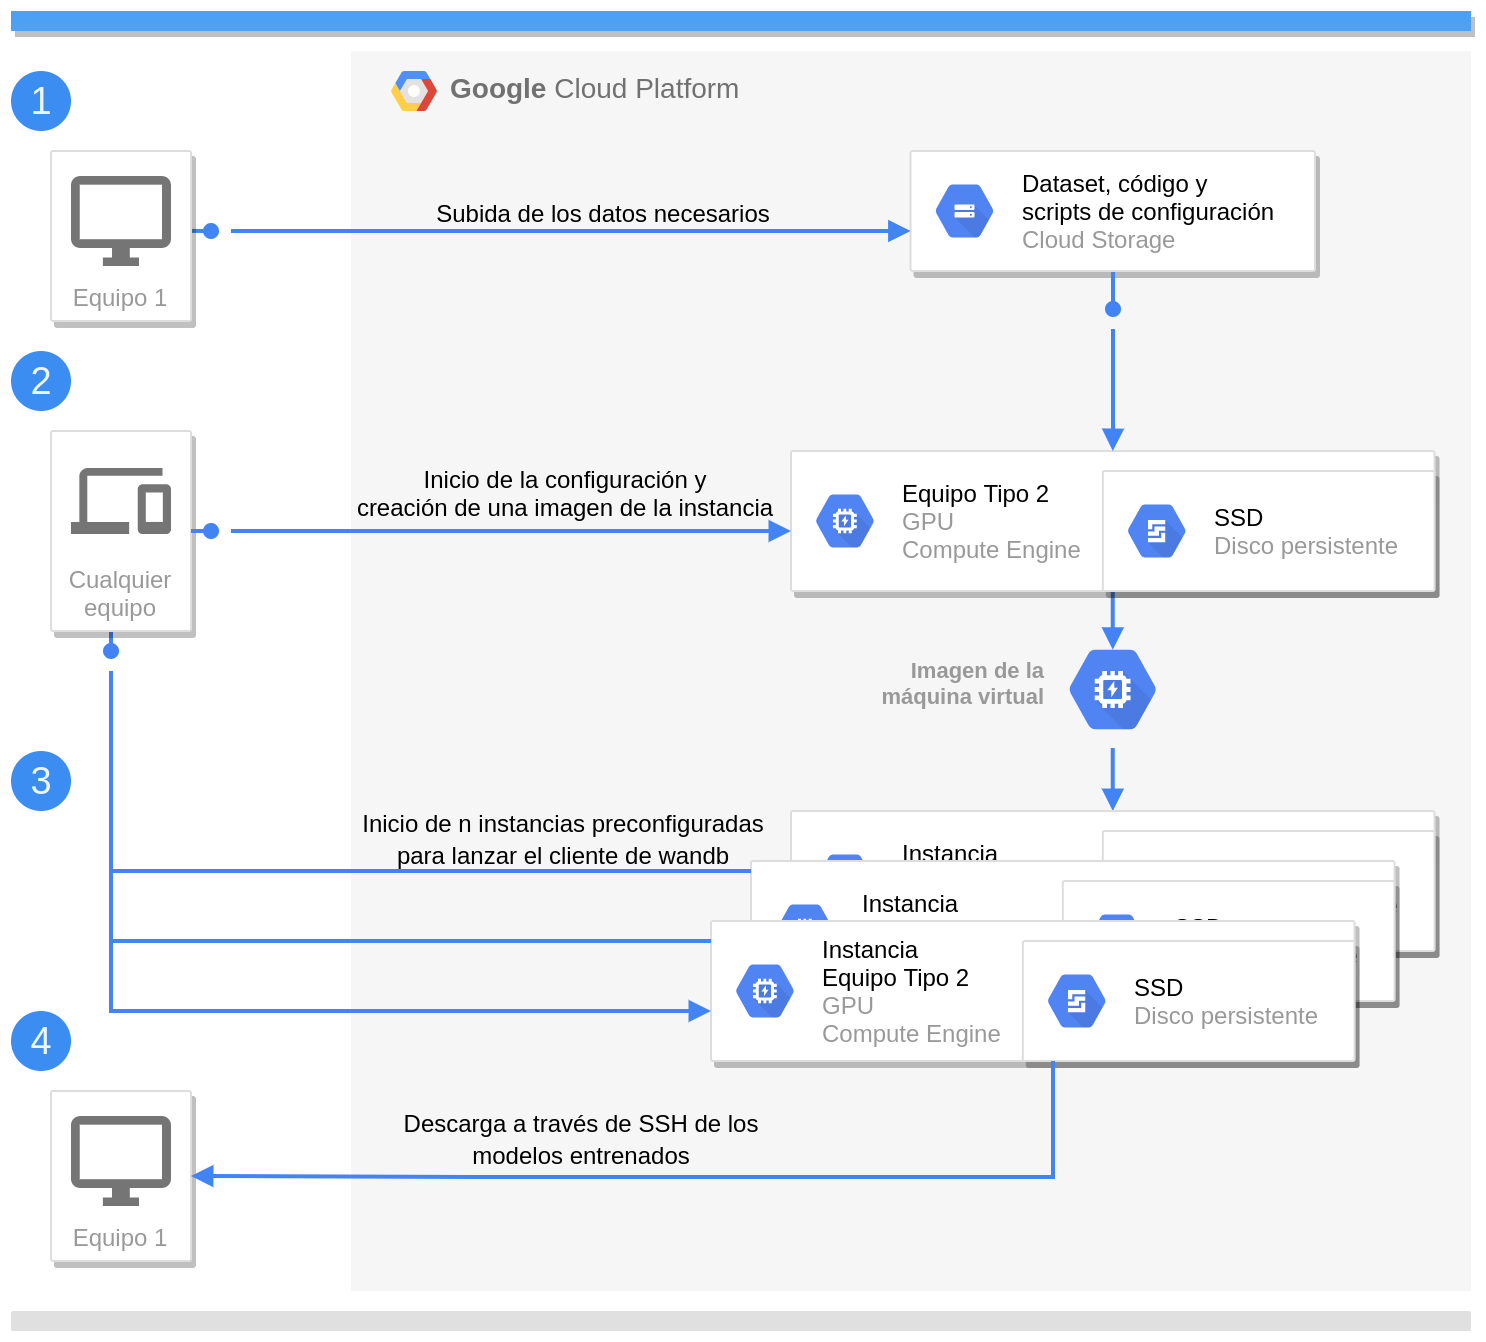
\includegraphics[width=\textwidth]{imagenes/cloud-diagram.png}
\caption{Esquema de la configuración llevada a cabo en la nube.}
\label{fig:cloud-diagram}
\end{figure}

\subsection{Arquitectura y capas}
Hablar de la arquitectura en concreto que se ha utilizado (DPT) apoyándose en todo lo que se haya explicado en el fundamento teórico. Explicar también las capas de atención que se han empleado en más detalle.
Apuntar como se hace para estimar la profundidad métrica en un dataset concreto (aquí o \textbf{en el apartado de arquitectura}).

\subsection{Warmstart}
Para acelerar lo máximo posible la convergencia del modelo durante el entrenamiento, se aprovechan en la medida de lo posible parámetros con sesgos inductivos ya aprendidos, es decir, parámetros de modelos ya entrenados. Más concretamente, los parámetros de los modelos a entrenar se inicializan con los valores de los parámetros del modelo DPT-Hybrid entrenado en MIX6, publicados en el artículo original de \textit{Dense Prediction Transformers} \cite{visiontransformersDPT}. 

Además, ya que en este trabajo se estudian diferentes modificaciones de dicho modelo, se emplea el método \texttt{load\_state\_dict()} de la clase \texttt{torch.nn.Module} con el parámetro \texttt{strict=False} para cargar los parámetros, evitando así que la carga falle si no coinciden una a una las capas en el modelo y las definidas en el archivo que se trata de cargar. En cuanto a las capas/conjuntos de capas que se han modificado y/o añadido, al no disponer del conjunto de datos MIX6 para preentrenarlas, se han inicializado con sus parámetros correspondientes tras ser entrenadas en ImageNet1K.

\todo[inline]{Comprobar esto entrenando el modelo de ResNet con los pesos de imagenet.}
Esta forma de proceder, sin embargo, origina un problema que se comentará más adelante en detalle, y es que como era de esperar, los modelos con menor porcentaje de su arquitectura modificada parten de una situación inicial ventajosa para la tarea de estimación de profundidad monocular (al estar preentrenados en MIX6).

\subsection{Data augmentation}
Hablar de data augmentation si se lleva a cabo, exponer las operaciones y justificarlas con regularización y generalización a casos nuevos, evitar que siempre se itere sobre las mismas imágenes.

\subsection{Entrenamiento}
Pese a que los autores del artículo de DPT \cite{} han publicado el código del modelo y sus pesos preentrenados en MIX6 y ajustados a NYUDepthv2 y KITTI, a día de hoy no han hecho público el \textit{script} de entrenamiento empleado. Por esto, ha sido necesario escribir el proceso de entrenamiento así como el \texttt{Dataset} de PyTorch con el que leer los datos de KITTI.

Para el \texttt{Dataset}, se crea una clase \texttt{KITTIDataset}\footnote{URL al repo?} que hereda de la clase abstracta base para conjuntos de datos que ofrece PyTorch, \texttt{torch.utils.data.Dataset}, y sobreescribe los métodos \texttt{\_\_len\_\_()} y \texttt{\_\_getitem\_\_()} de forma que estos se adapten a la estructura de directorios y nombres de las imágenes de sus anotaciones. Al sobreescribir estos métodos, es posible crear un \texttt{torch.utils.data.Dataloader} de forma directa, pasando las imágenes y las etiquetas a los modelos aprovechando las herramientas de PyTorch. En el método \texttt{\_\_getitem\_\_()}, además, se aplican las transformaciones necesarias a los datos, así como el \textit{Data Augmentation}.

En cuanto al \textit{script} de entrenamiento\footnote{URL de train.py y train\_ utils.py?}, se tienen en cuenta una serie de factores para acelerar el proceso lo máximo posible:
\begin{itemize}

\item \textbf{Número de trabajadores en el \texttt{Dataloader}}: Con el objetivo de asegurar que la limitación en la velocidad de entrenamiento sea el procesamiento en la GPU, se cambia el valor del parámetro \texttt{num\_workers} del constructor del \texttt{Dataloader} de entrenamiento a 8. Este parámetro, controla el número de procesos que se lanzan en paralelo para leer los datos del disco y preprocesarlos.

\item \textbf{\texttt{pin\_memory}}: También en el constructor del \texttt{Dataloader}, es posible activar \texttt{pin\_memory}, parámetro desactivado por defecto. Este parámetro, acelera la transferencia a la memoria de la GPU de los datos cargados en memoria (RAM) por la CPU \cite{harris2012}. De forma resumida, lo que habilita este parámetro es que la carga de datos se haga en memoria no paginable (\textit{pinned}) a la que la GPU accede directamente, evitando así cargar los datos en una zona de memoria paginable y transferir estos a una \textit{pinned memory} temporal cada vez que la GPU quiere leerlos para transferirlos a su propia memoria.

\item \textbf{\texttt{torch.backends.cudnn.enabled y \texttt{torch.backends.cudnn.benchmark}}}: Estas dos opciones, se activan para asegurar, respectivamente, que se use CuDNN en la ejecución del modelo y que se ejecuten al comienzo del \textit{script} distintas implementaciones de algoritmos de convolución para emplear el más rápido en el sistema actual.

\item \textbf{\textit{Mixed precision}}: Ya mencionado en el apartado TODO, pese a que finalmente se ha descartado su uso en el entrenamiento debido a la inestabilidad numérica que introducía y los fallos que ocasionaba, el \textit{script} de entrenamiento incluye la opción de activar el uso de precisión mixta con el escalado pertinente.
\end{itemize}

\todo[inline]{Medir y hacer una gráfica de la influencia de cada uno de estos en un trozo de epoch}

El entrenamiento en sí, se ha llevado a cabo empleando como optimizador \texttt{AdamW} con $lr = 1e-5$, $\beta_1 = 0.9$, $\beta_2 = 0.999$, $\epsilon = 1e-8$ y $\textit{weight decay} = 0.01$ con un número de épocas fijado a 20 (el entrenamiento se detiene en caso de que la función de pérdida se desestabilice y se vuelva $\pm \infty$). Como se ha mencionado en el apartado TODO, el tamaño de lote es uno, pero el \textit{script} de entrenamiento implementa la posibilidad de usar acumulación de gradientes para simular tamaños de lote mayores. La función de pérdida, ha sido TODO, (citar y Ecuación X). Por último, durante el entrenamiento se ha empleado la función \texttt{torch.nn.utils.clip\_grad\_value\_} con un \texttt{clip\_value} de 0.5, que se encarga de limitar los valores de los gradientes en función de su valor, para limitar considerablemente las posibilidades de que explotasen los gradientes del modelo haciendo que se desestabilizase su entrenamiento.


%\todo[inline]{Pseudocódigo del script de entrenamiento}
%\begin{algorithm}
%\floatname{algorithm}{Pseudocódigo}
%\caption{My algorithm}\label{euclid}
%\begin{algorithmic}[1]
%
%\For{\texttt{época = 1 a 20}}
%\State \texttt{train()}
%\State \texttt{val()}
%\If {\texttt{época mod 5 == 0}}
%\State {\texttt{guardaModelo()}}
%\EndIf
%\EndFor
%\end{algorithmic}
%\end{algorithm}


\todo[inline]{En la tabla de resultados generales sumar las horas de entrenamiento y ya de paso mencionar el total de horas atribuyendolas a otros entrenamientos y pruebas/experimentos (en la sección de resultados)}

\subsection{Reducción de tamaño de la entrada}
Para acelerar DPT, lo primero que se modificó fue el tamaño de la entrada. Los resultados de la publicación original calculan la profundidad en el conjunto de evaluación de KITTI con las imágenes en su tamaño original, 1216x352, para reducir el consumo de memoria del modelo durante su entrenamiento, así como acelerar entrenamiento e inferencia, se han añadido dos operaciones de cambio de tamaño: una al principio de la red que reduce el tamaño de las imágenes a 640x192 píxeles, y otra al final de la red que reescala la salida al tamaño original. La primera operación emplea como método de interpolación el algorítmo \texttt{INTER{\_}AREA} de OpenCV, que TODO y está recomendado para reducir el tamaño de imágenes ya que proporciona resultados sin efecto Moire; la operación que amplia la salida al tamaño de la imagen original, por otro lado, emplea interpolación bicúbica, que ofrece los mejores resultados pese a ser más lenta, ya que el tiempo empleado en las operaciones de reescalado es despreciable en comparación con el tiempo de inferencia de la red.

\todo[inline]{Medir el tiempo que está escalando y haciendo inferencia para justificar la frase del final}
\todo[inline]{Hacer una comparación de velocidad de inferencia con la imagen en grande y con la imagen en pequeño}
\todo[inline]{Entrenar un modelo con la imagen grande para ver como afecta? Podría ser solo uno, similar a la prueba que se quiere hacer con el resnet entrenado en imagenet}
\todo[inline]{Explicar inter{\_}area, citarlo? explicar en una nota al pie qué es el efecto moire?}

% https://medium.com/@wenrudong/what-is-opencvs-inter-area-actually-doing-282a626a09b3

\subsection{Número de cabezas}
Hablar del cambio en el número de cabezas
\todo[inline]{Citar y justificar esta dirección de búsqueda con el paper de are 16 heads better than 1}

\subsection{Capas de atención eficiente}
Cambio de las capas, hacer una gráfica midiendo en función del tamaño de la cadena la velocidad en la que pasa por una de estas capas? Puede ser interesante. (Sería para imágenes mayores)

\todo[inline]{Hacer un estudio del incremento de velocidad en función del tamaño de los tokens, es posible que haga falta usar una máquina de Google Cloud para esto, se puede coger una gorda con mucha mucha memoria, habría que incluirla en el apartado de hardware, también se podría usar para el cálculo de el flujo máximo de imagenes (una A100/P100). Se podría usar la misma imagen en teoría, si sale bien mencionarlo también en el apartado de Docker o en el de Google Cloud}

\subsection{Cambio en los hooks del transformer y eliminación de las capas de atención posteriores}

Hablar del cambio en los hooks, en el paper original se valora el cambio de hooks en la etapa convolucional, pero no en el transformer, se estudian 0,1; 2,5; 8,11

Al modificar las capas del transformer de las que se cogen las activaciones para pasarlas a la etapa de fusión convolucional, se abre la posibilidad de eliminar aquellos bloques de atención que ya no se usan. Esta modificación, además de acelerar el entrenamiento e inferencia del modelo, reduce su tamaño considerablemente, tanto a la hora de almacenar sus parámetros como a la hora de cargarlo en memoria para desplegarlo en una aplicación real. En la Figura \ref{fig:attention_block_num}, se puede apreciar la modificación del ViT empleado en DPT: a la izquierda está el encoder tal y como se encuentra en el trabajo de DPT, con los \textit{hooks} en los bloques 8 y 11, sin eliminar ninguno de los parámetros del transformer, y con la inferencia recorriendo los 12 bloques de atención; a la derecha, por otro lado, está una de las opciones valoradas para este hiperparámetro de la arquitectura, donde los hooks se sitúan en la salida de los bloques 0 y 1 del ViT. De esta forma, en el ejemplo, los parámetros a partir del segundo bloque de atención pueden eliminarse ya que la inferencia del modelo solo llega hasta este segundo bloque.

\todo[inline]{Hacer una comparación del tamaño del modelo cuando se eliminan los pesos}
\todo[inline]{Hacer una comparación de los resultados en validación en función de los hooks}
\todo[inline]{Hacer una comparación de la velocidad de inferencia en función de los hooks empleados}
\todo[inline]{Mencionar en la discusión que esto está muy bien porque no están reduciendo la complejidad de la atención, te la estás cargando directamente}
\todo[inline]{Meter el código aquí o una referencia a las partes del código donde se encuentra este cambio?}

\begin{figure}[H]
\centering
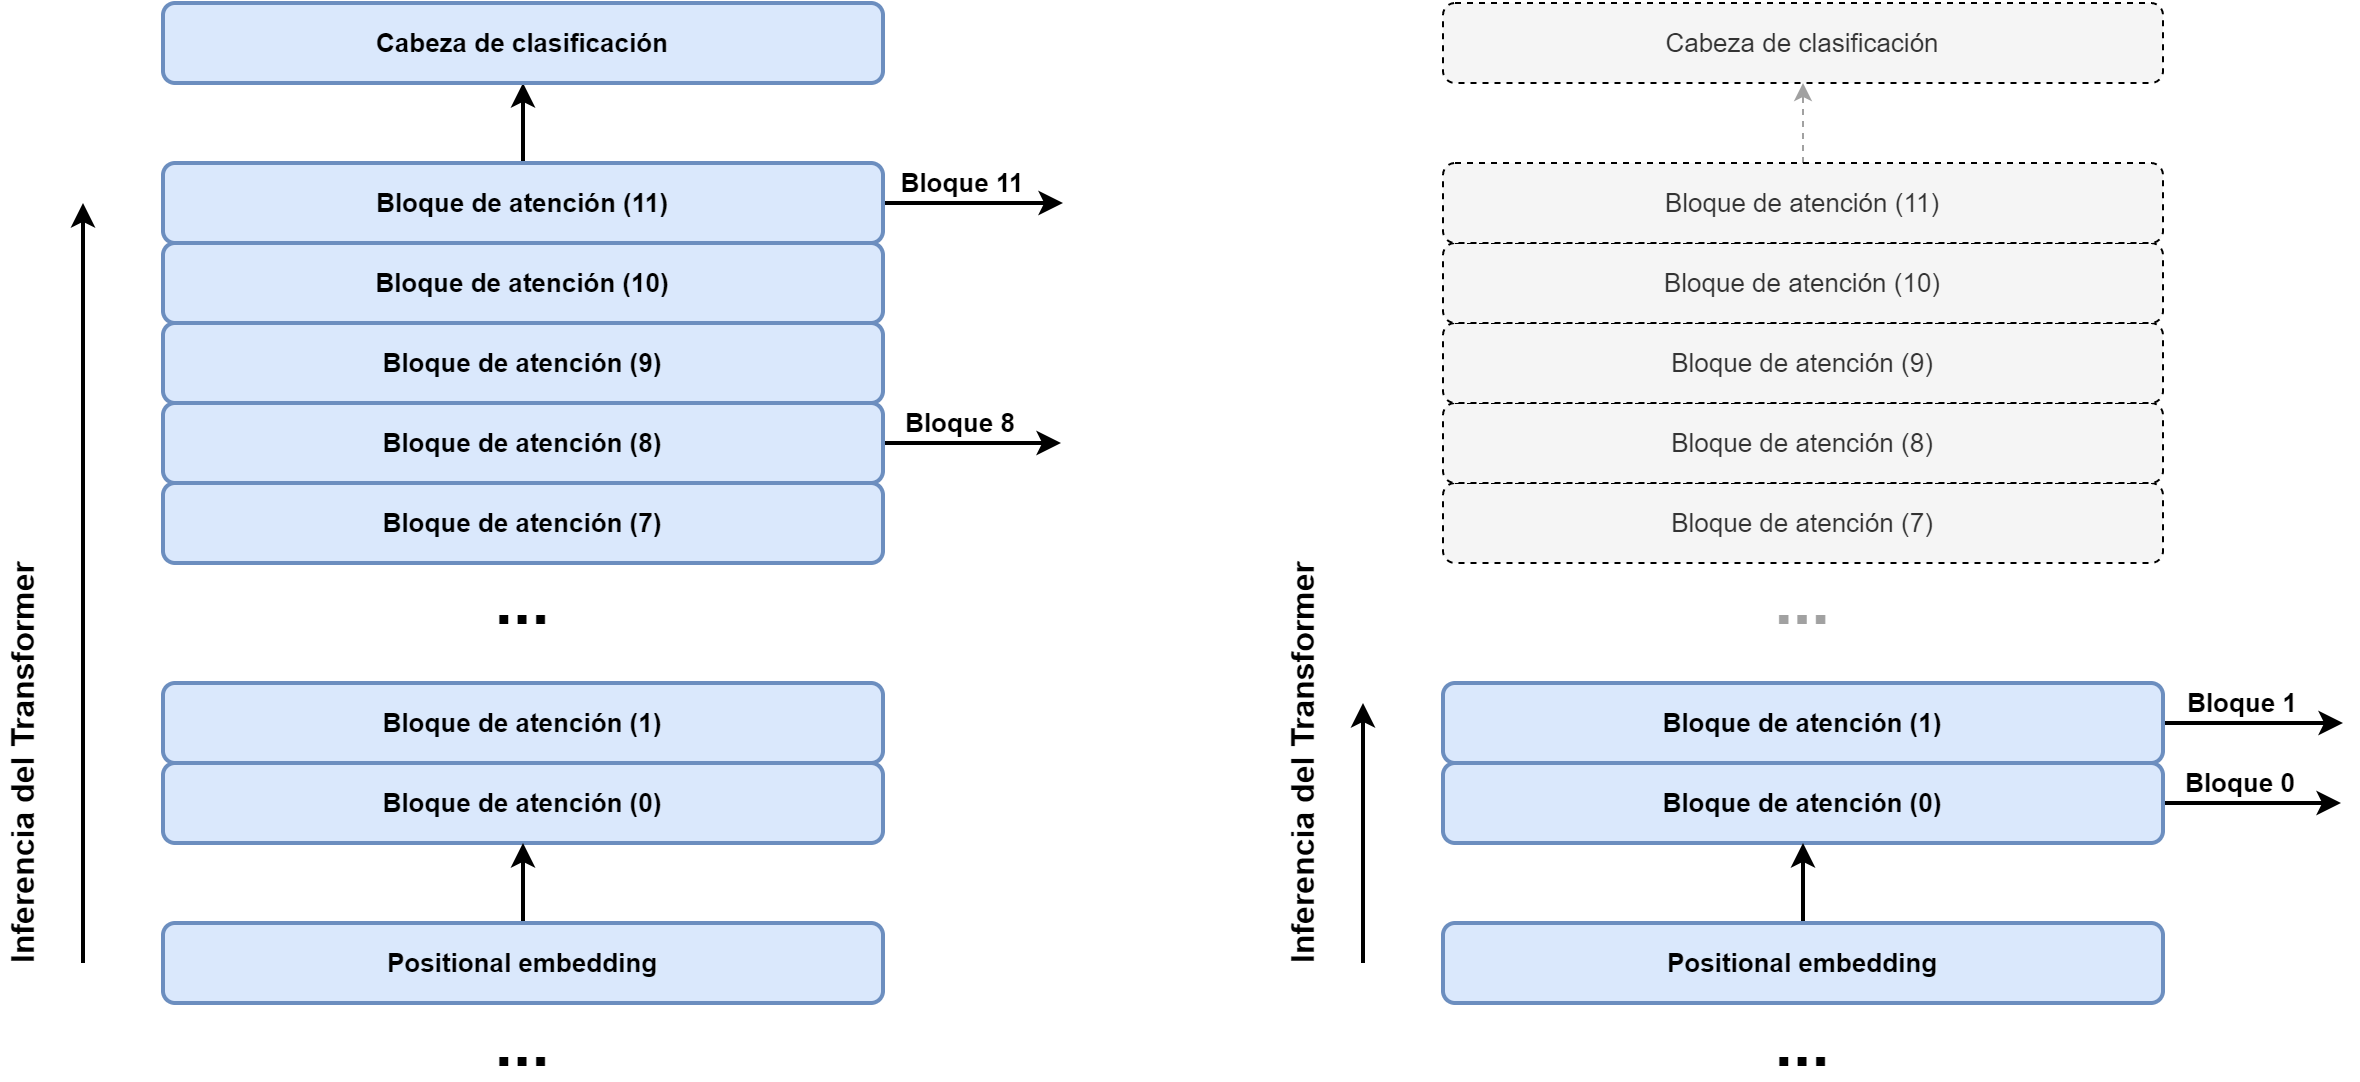
\includegraphics[width=\textwidth]{imagenes/DPT-cambio-bloques-transformer.png}
\caption{Cambio en el número de bloques de atención.}
\label{fig:attention_block_num}
\end{figure}



\begin{figure}[H]
\centering
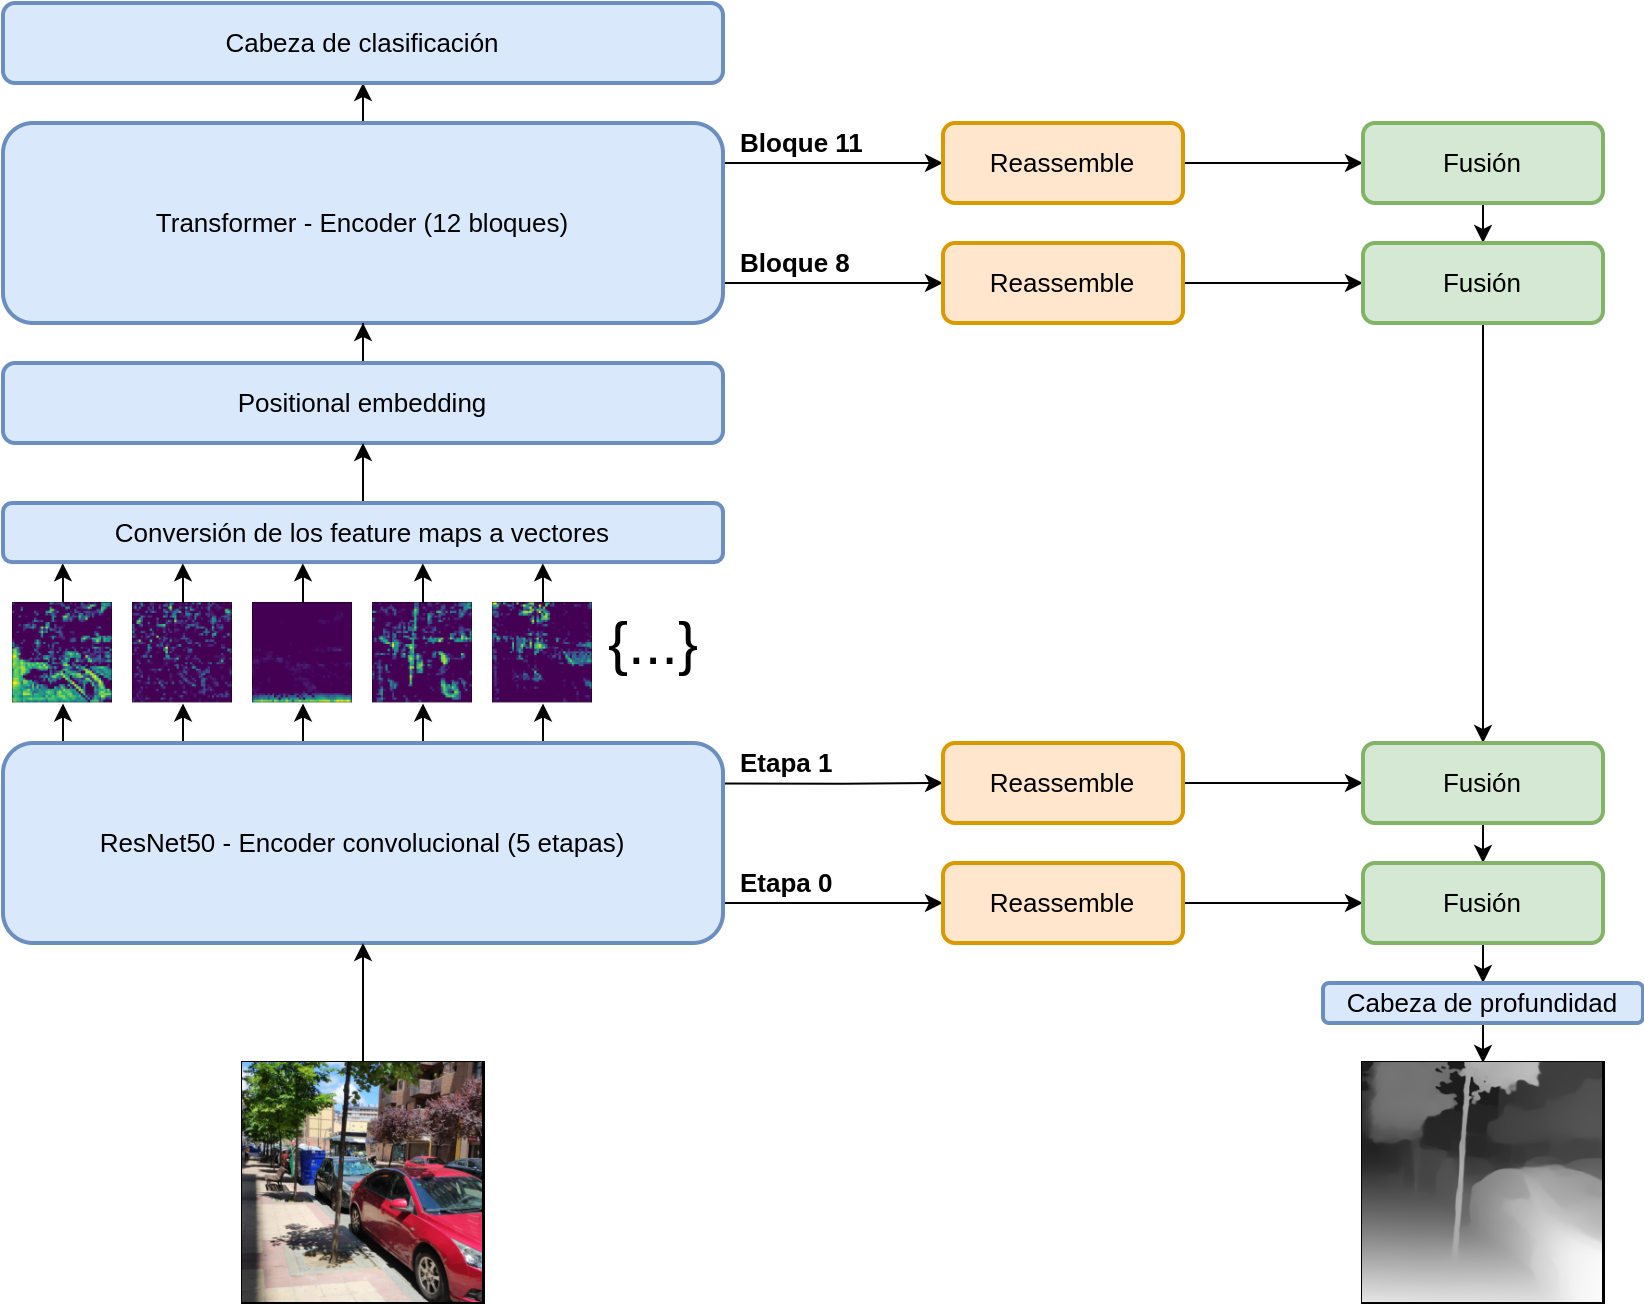
\includegraphics[width=\textwidth]{imagenes/DPT-general.png}
\caption{Arquitectura general DPT.}
\label{fig:dpt-general}
\end{figure}

\begin{figure}[H]
\centering
\includegraphics[width=\textwidth]{imagenes/DPT-modificado-general.png}
\caption{Arquitectura general DPT tras las modificaciones.}
\label{fig:dpt-mod-general}
\end{figure}

\subsection{Cambio del backbone convolucional}
El último cambio estudiado en este proyecto es el del backbone convolucional del Hybrid ViT. En el modulo propuesto en la publicación original, se elige como backbone una ResNet50v2, de la que se extraen las activaciones en los bloques 0 y 1, que tienen un tamaño TODO de 256 y 512, quedando así TODO de tamaños [256, 512, 768, 768]. Por otro lado, la salida de la última capa de la ResNet50v2, es decir, la entrada de los bloques de atención, tiene forma [n, c, h, w], donde n es el número de imágenes en el batch (batch size), c el número de canales (en este caso mapas de características), que son 1024 por como está diseñada la arquitectura, y por último, h y w, que son la altura y anchura de los mapas de características y son iguales a las dimensiones de la imagen de entrada divididas 4 veces entre 2. Después de la ResNet, hay una capa de proyección que no es más que una capa convolucional con kernels de tamaño 1x1 y stride 1x1, con 1024 canales de entrada y 768 canales de salida. Este tipo de capas, realmente son 786 kernels de 1x1x1024, por lo que al convolucionar cada uno de ellos la entrada, se obtienen 768 mapas de características del mismo tamaño que los de la entrada. Los 768 mapas de características resultantes, se aplanan en tensores de forma [n, 768, h/8 * w/8] y se transponen de forma que la entrada sea de tipo [n, t, 768], donde 768 es el tamaño de los tokens de los bloques de atención y t el número de tokens extraidos de la imagen. De esta forma, a mayor tamaño de imagen mayor será el número de tokens, pero la dimensión de estos permanece constante.

\todo[inline]{Hablar de las convoluciones con kernels 1x1 arriba en vez de aquí?}

A modo de ejemplo, supongamos una entrada de una sola imagen de tamaño 384x384: la salida de la ResNet50v2 tendrá la forma [1, 1024, 24, 24]. Esta salida atraviesa la capa de proyección y pasa a tener forma [1, 768, 24, 24]. Estos mapas de características se aplanan en un tensor [1, 768, 576] que se traspone para obtener la forma [1, 576, 768], que equivale a 576 tokens de dimensión 768. Una vez llegados a este punto, el tensor está listo para pasar a los bloques de atención del transformer.

Por otro lado, la arquitectura EfficientNet-B0, alternativa usada en las pruebas de este trabajo, proporciona una salida (antes de la capa de global pooling) de forma [n, c, h, w] donde n vuelve a ser el número de imágenes procesadas en paralelo, el número de mapas de características es en este caso 1280, y la altura y anchura se corresponden con las de las imágenes de entrada divididas 5 veces entre 2. Es decir: [n, 1280, h/16, w/16]. Para poder sustituir el backbone convolucional del Hybrid ViT sin tener que cambiar el tamaño de todas las capas de atención (para poder aprovechar los pesos preentrenados), se sustituye la capa de proyección mencionada en el párrafo superior, que recordemos era una capa convolucional con kernels de tamaño 1x1 por una capa de convolución transpuesta. Esta capa de convolución transpuesta, cumple dos funciones fundamentales: la primera, transforma los 1280 mapas de características en 768; y la segunda, al tener un kernel de tamaño 2x2 y un stride también de 2x2, consigue que las dimensiones de estos mapas de características se multiplen exactamente por 2 en ambas dimensiones, convirtiendo la entrada [n, 1280, h/16, w/16] en [n, 1280, h/8, w/8], que es lo que espera la etapa que aplana los mapas de características y transpone el tensor para obtener de nuevo la entrada preparada para los bloques de atención de forma [n, t, 768] donde t vuelve a ser el número de tokens que pasan al transformer, cada uno de dimensión 768.

\todo[inline]{Explicar bien y añadir en el parrafo de efficientnet el tamaño que tienen los hooks de la red convolucional}
\todo[inline]{Meter alguna imagen para explicar todo este apartado}
\todo[inline]{Decir lo de que se ha modificado la carga de pesos del modelo}
\todo[inline]{Decir (y luego repetir) que efficientnet no está preentrenada en mix y que esto evidentemente afectará a los resultados}


% En los resultados hablar de la distribución de los pesos antes y después de convertir el modelo si es pertinente, hacer una especie de estudio de ablación si se puede entrenar modelos, etc. Puede estar interesante quitar cabezas de atención, quitar bloques de atención, ver como afecta al tamaño dle modelo, su rendimiento (velocidad y métricas)...

\clearpage
\capitulo{5}{Resultados}

\begin{wrapfigure}{r}{0.45\textwidth}
\vspace{-15pt}
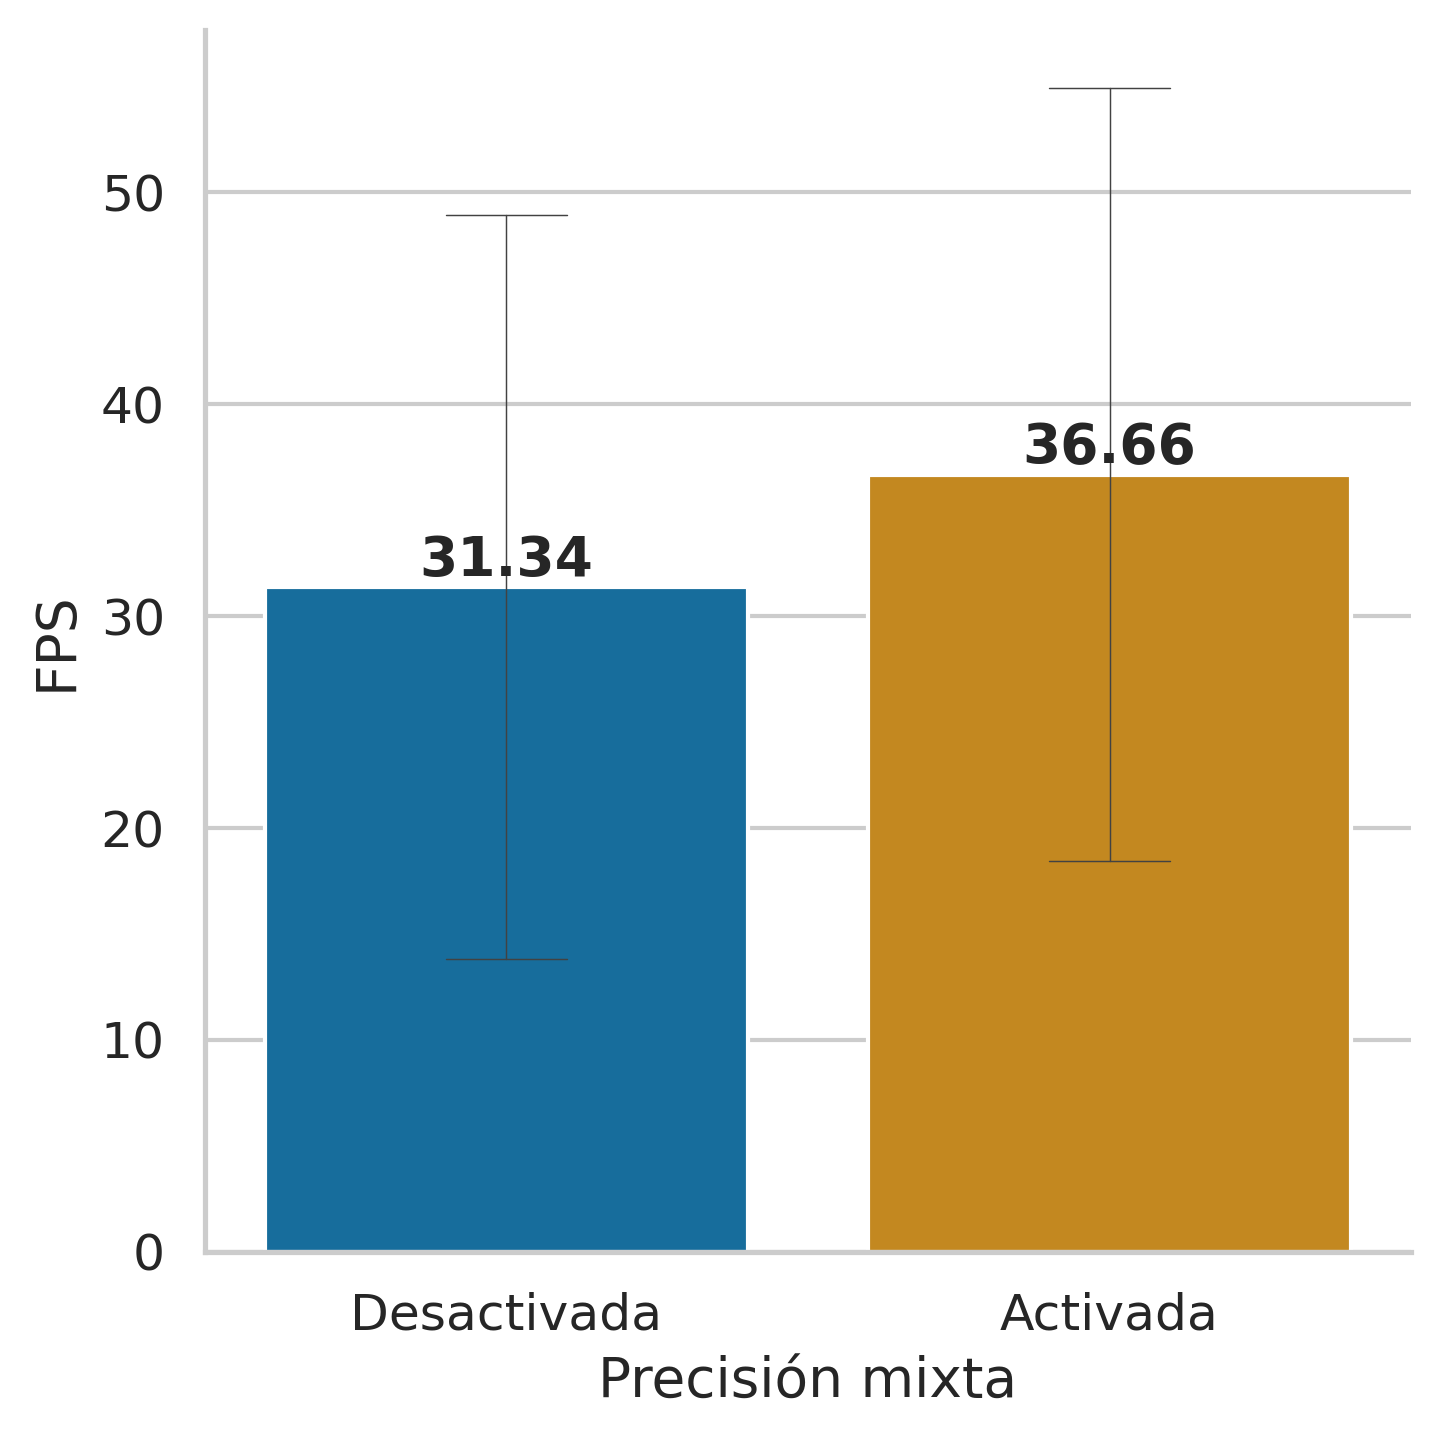
\includegraphics[width=0.95\linewidth]{imagenes/Resultados/mixed_precision.png} 
\caption{FPS promedios de los modelos en función de la precisión usada para realizar la inferencia. Las barras grises representan la desviación estándar de las medidas.}
\label{fig:resultados-mixed-precision}
\end{wrapfigure}

En este capítulo se exponen los resultados obtenidos en el conjunto de validación tras entrenar las arquitecturas con las modificaciones planteadas. Tal y como se plantearon en el \Cref{modelos-a-entrenar}, los experimentos han consistido en entrenar $36$ modelos definidos por el producto cartesiano de las opciones: (ResNet50, EfficientNet-B0) como \textit{backbone}, (Atención estándar, Atención \textit{Performer}) como mecanismo de atención, ($1$, $12$, $24$) como número de cabezas de atención, y ([$0$, $1$], [$2$, $5$], [$8$, $11$]) como bloques de atención de los que se toma la salida para que sea la entrada del \textit{decoder}. En este capítulo, además de las métricas que miden la exactitud de las salidas, se presentan también métricas de velocidad de inferencia. Para medir este último grupo de variables, tras comprobar que los resultados numéricos en la salida de los modelos eran idénticos, se emplea precisión mixta para aumentar la velocidad lo máximo posible (\Cref{fig:resultados-mixed-precision}).


\section{Resultados cuantitativos}

\subsection{Reducción del tamaño de la entrada}

Dado que el entrenamientos de los modelos - por limitaciones materiales y temporales - se ha llevado a cabo reduciendo el tamaño de la entrada, no es posible comparar los resultados obtenidos para cada una de las modificaciones de la arquitectura con su modelo entrenado con las imágenes en su tamaño original.

\begin{wrapfigure}{l}{0.45\textwidth}
\vspace{-15pt}
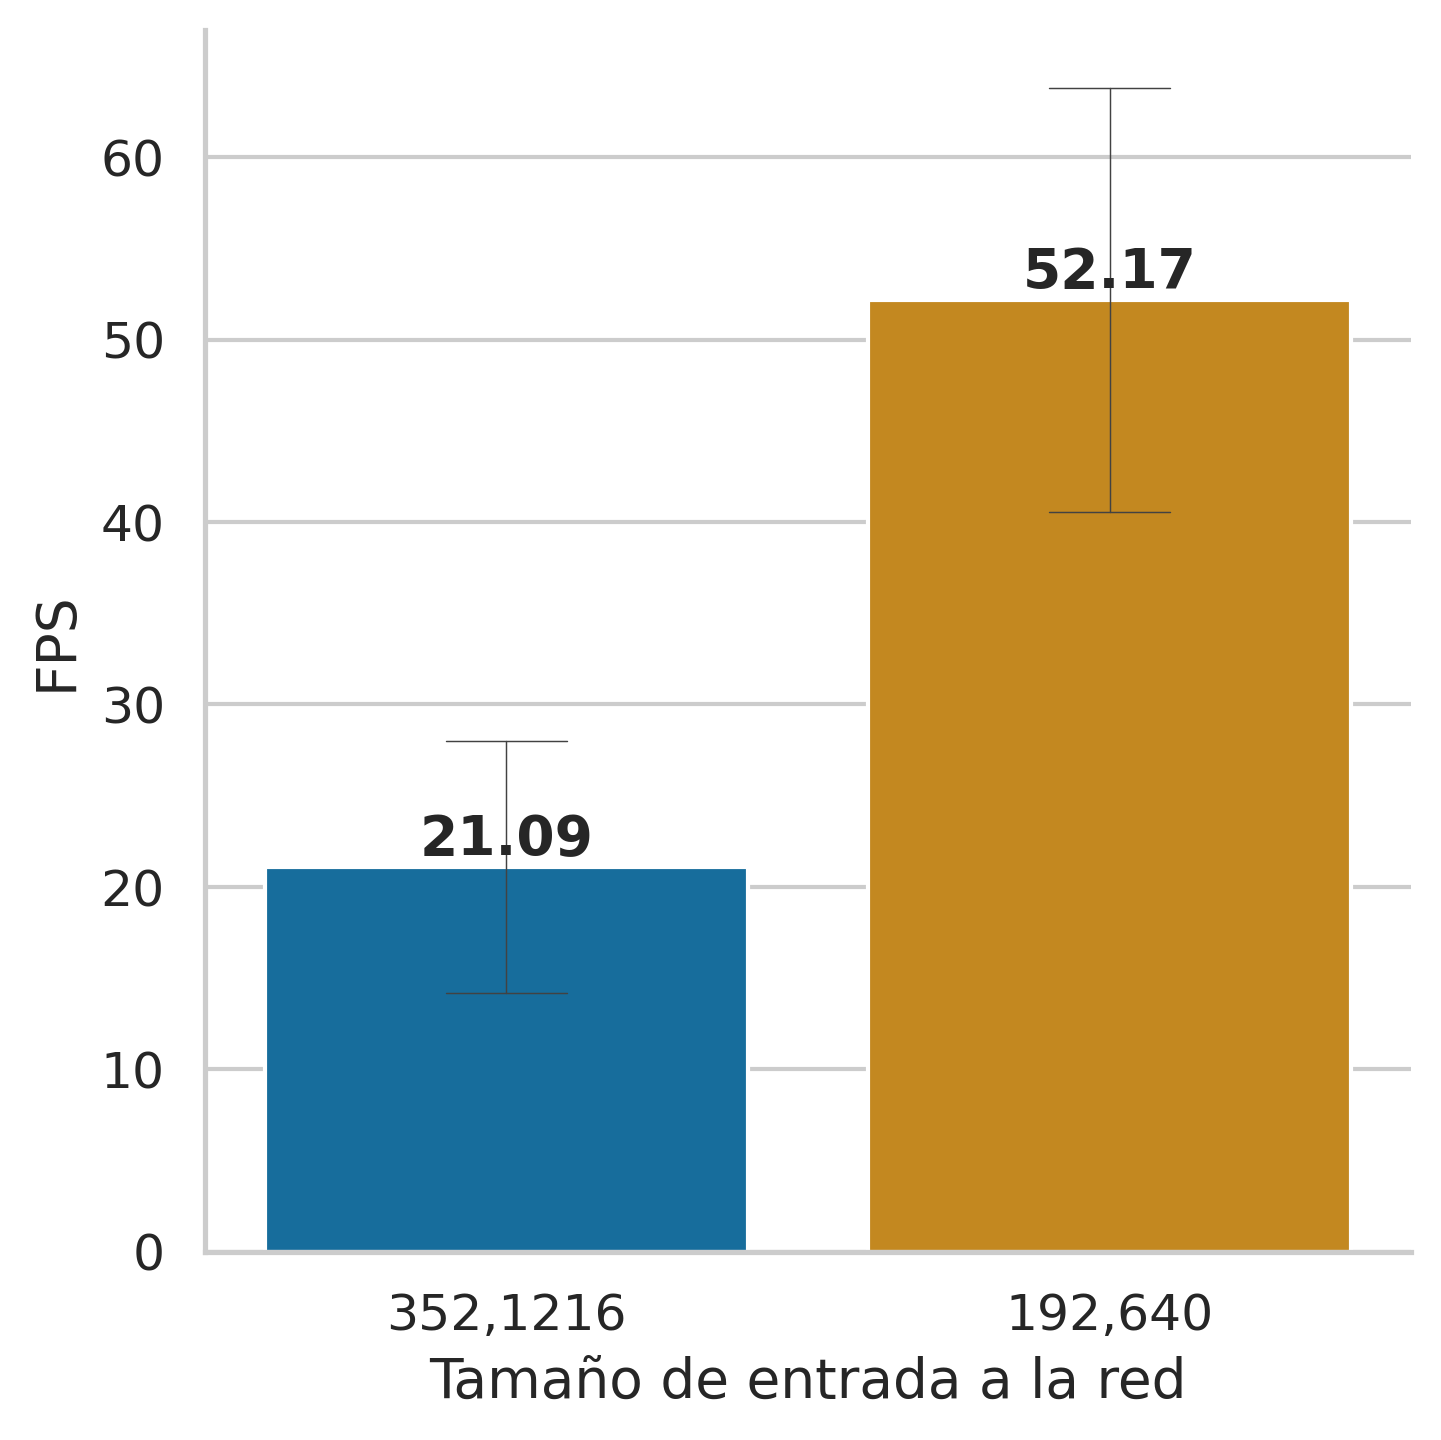
\includegraphics[width=0.95\linewidth]{imagenes/Resultados/velocidad_inferencia_entrada.png} 
\caption{FPS medios de los modelos en función del tamaño de su entrada. Las barras grises representan la desviación estándar de las medidas.}
\label{fig:resultados-inf-tam-entrada}
\end{wrapfigure}

Sin embargo, la medida de la velocidad de inferencia sí que es posible obtenerla independientemente de que los pesos correspondan al modelo entrenado o no. En la \Cref{fig:resultados-inf-tam-entrada} se puede apreciar la diferencia en función del tamaño de entrada de los FPS promedio de todas las modificaciones realizadas sobre el modelo DPT. El valor de la izquierda, corresponde al tamaño con el que se evalúa KITTI en la publicación original \cite{visiontransformersDPT}, mientras que el de la derecha es la reducción de tamaño establecida en este trabajo. Dado que este cambio es significativo y es, en términos de magnitud, el que mayor aceleración media conlleva ($\times2.47$), en las siguientes Figuras que representen los FPS en función de los otros cambios introducidos en el trabajo se presentarán los datos tanto con el tamaño de entrada original como con el tamaño de entrada reducido para poder así valorar también la mejora de rendimiento que conllevaría la modificación si no se hubiese reducido el tamaño de la entrada.



















\subsection{Cambio del backbone convolucional}\label{resultados-cuantitativos-backbone}
El cambio del \textit{backbone} convolucional usado para extraer los mapas de características, como era de esperar, también influye en la velocidad de inferencia de la red. En la \Cref{fig:resultados-inf-backbone}, es posible ver el incremento en los FPS promedio entre los modelos con ResNet50 y los modelos con EfficientNet-B0.

\begin{figure}[H]
\centering
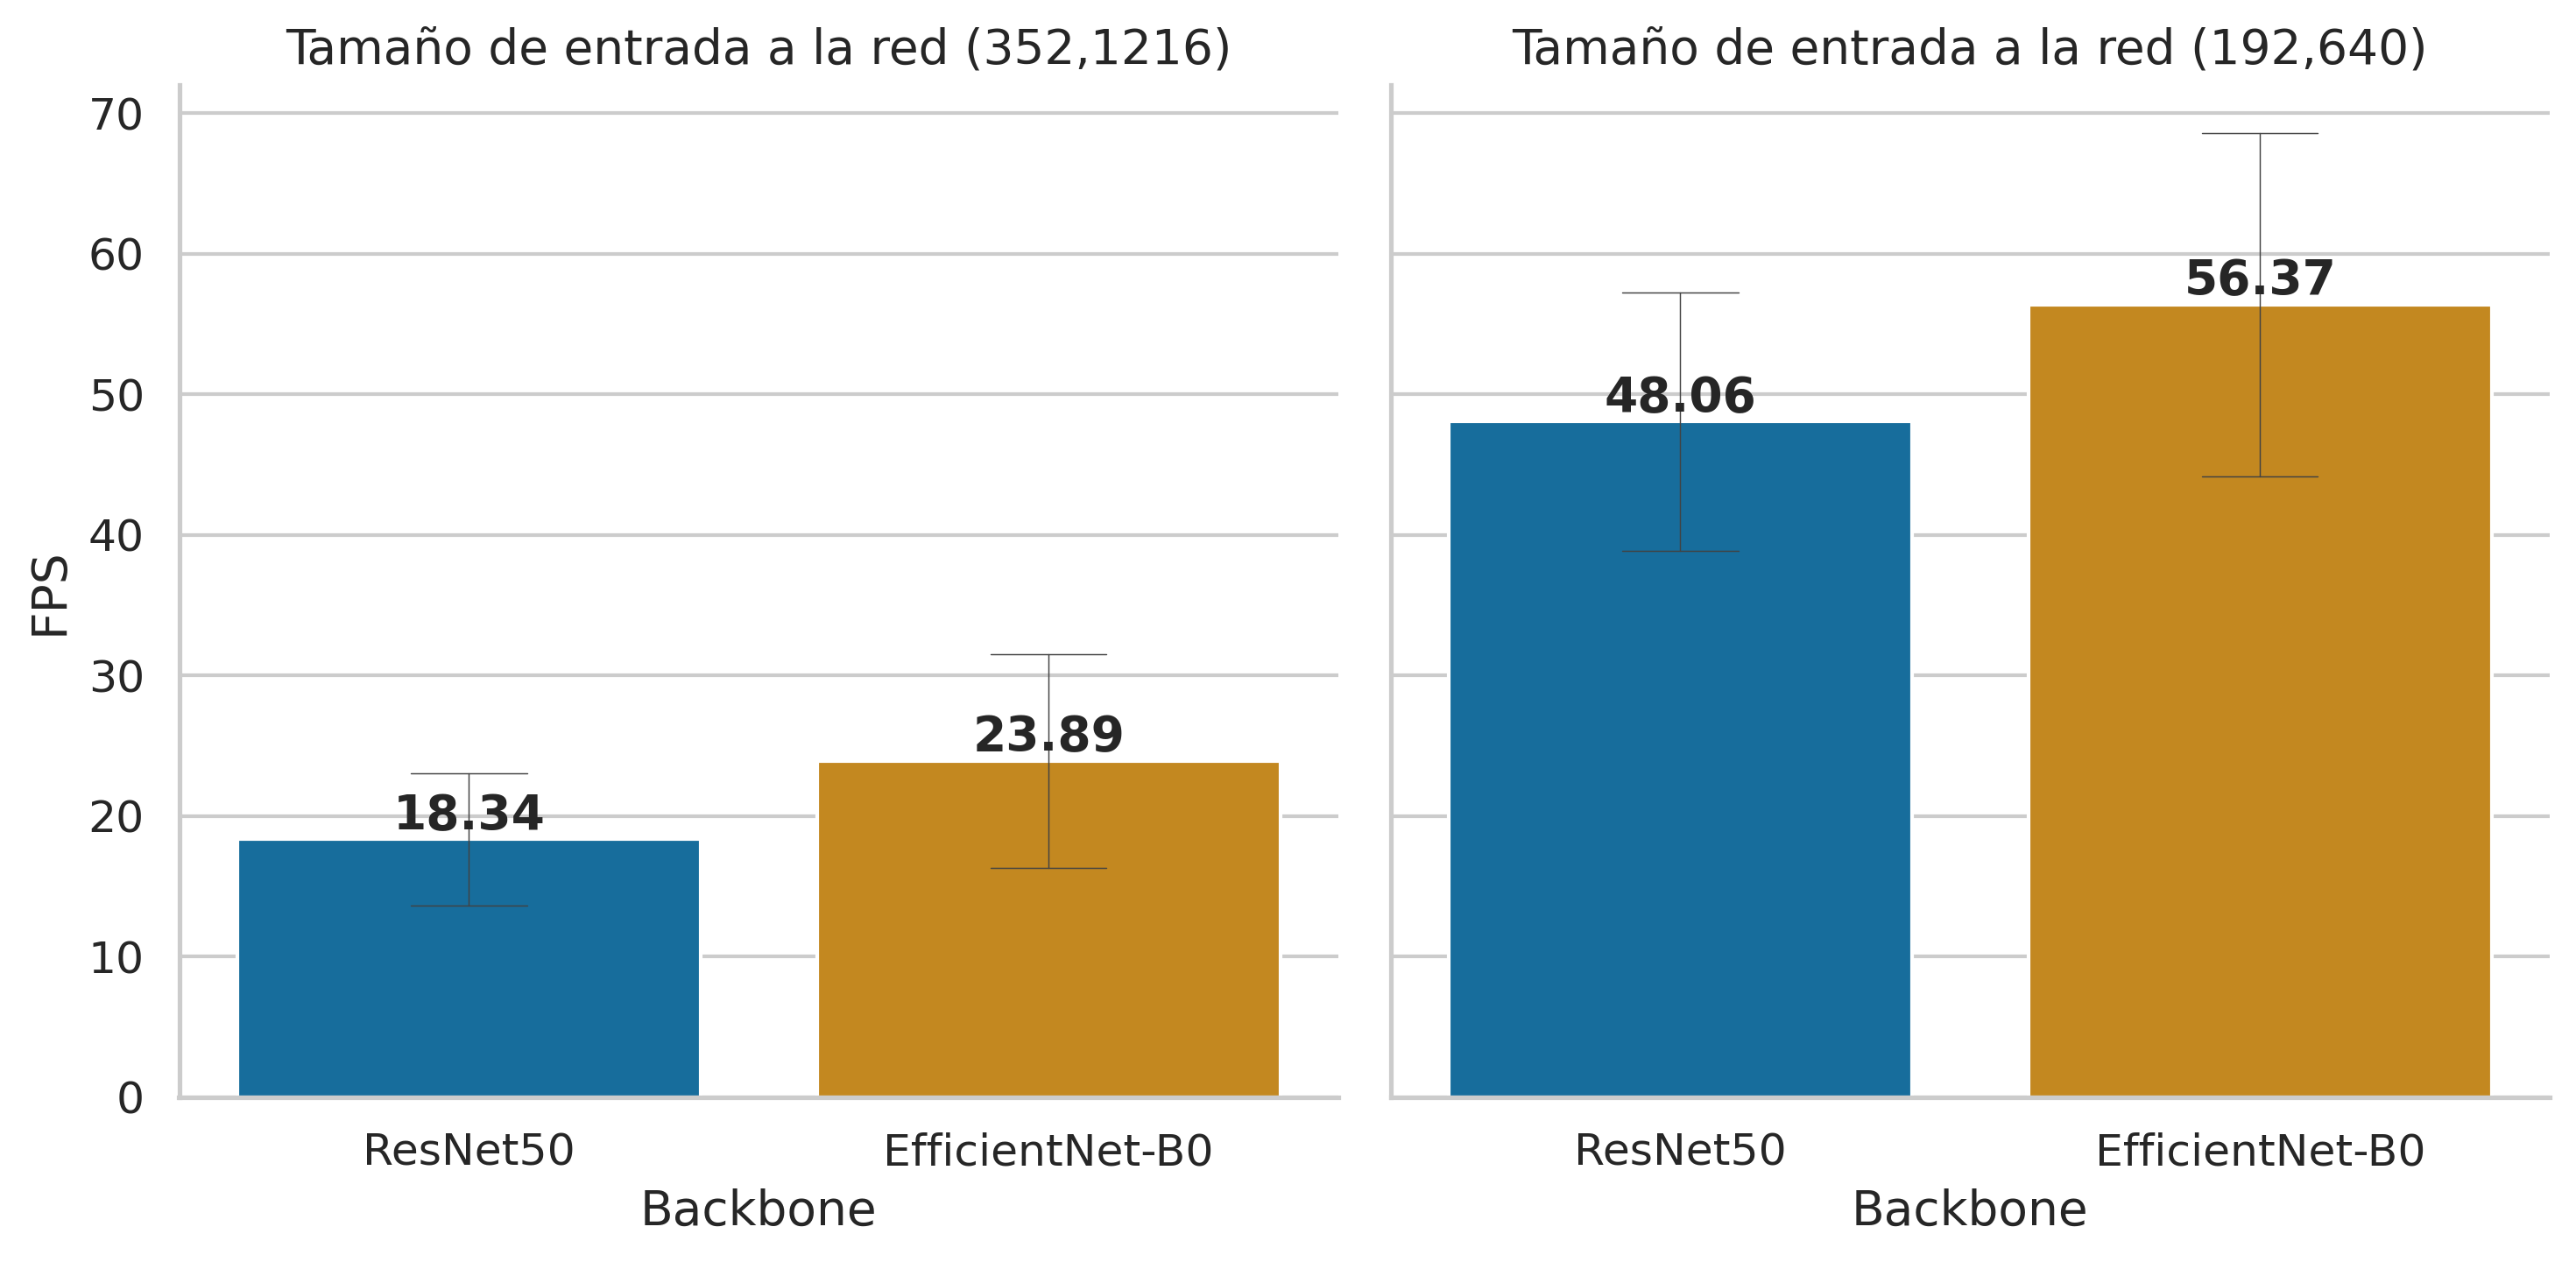
\includegraphics[width=0.8\linewidth]{imagenes/Resultados/velocidad_inferencia_backbone.png} 
\captionsetup{width=.8\linewidth}
\caption{FPS medios de los modelos en función del \textit{backbone} utilizado y del tamaño de la entrada. Las barras grises representan la desviación estándar de las medidas.}
\label{fig:resultados-inf-backbone}
\end{figure}

A pesar de que el incremento de velocidad es positivo, existe un problema asociado a la modificación del \textit{backbone}. De todas las modificaciones desarrolladas y estudiadas en este trabajo, el cambio de \textit{backbone} domina de forma muy considerable el deterioro de la calidad de los resultados, esto se puede ver claramente, por ejemplo, en la comparación del error logarítmico invariante a la escala (SIlog) disponible en la \Cref{fig:SIlog-validation}.

\begin{figure}[H]
\centering
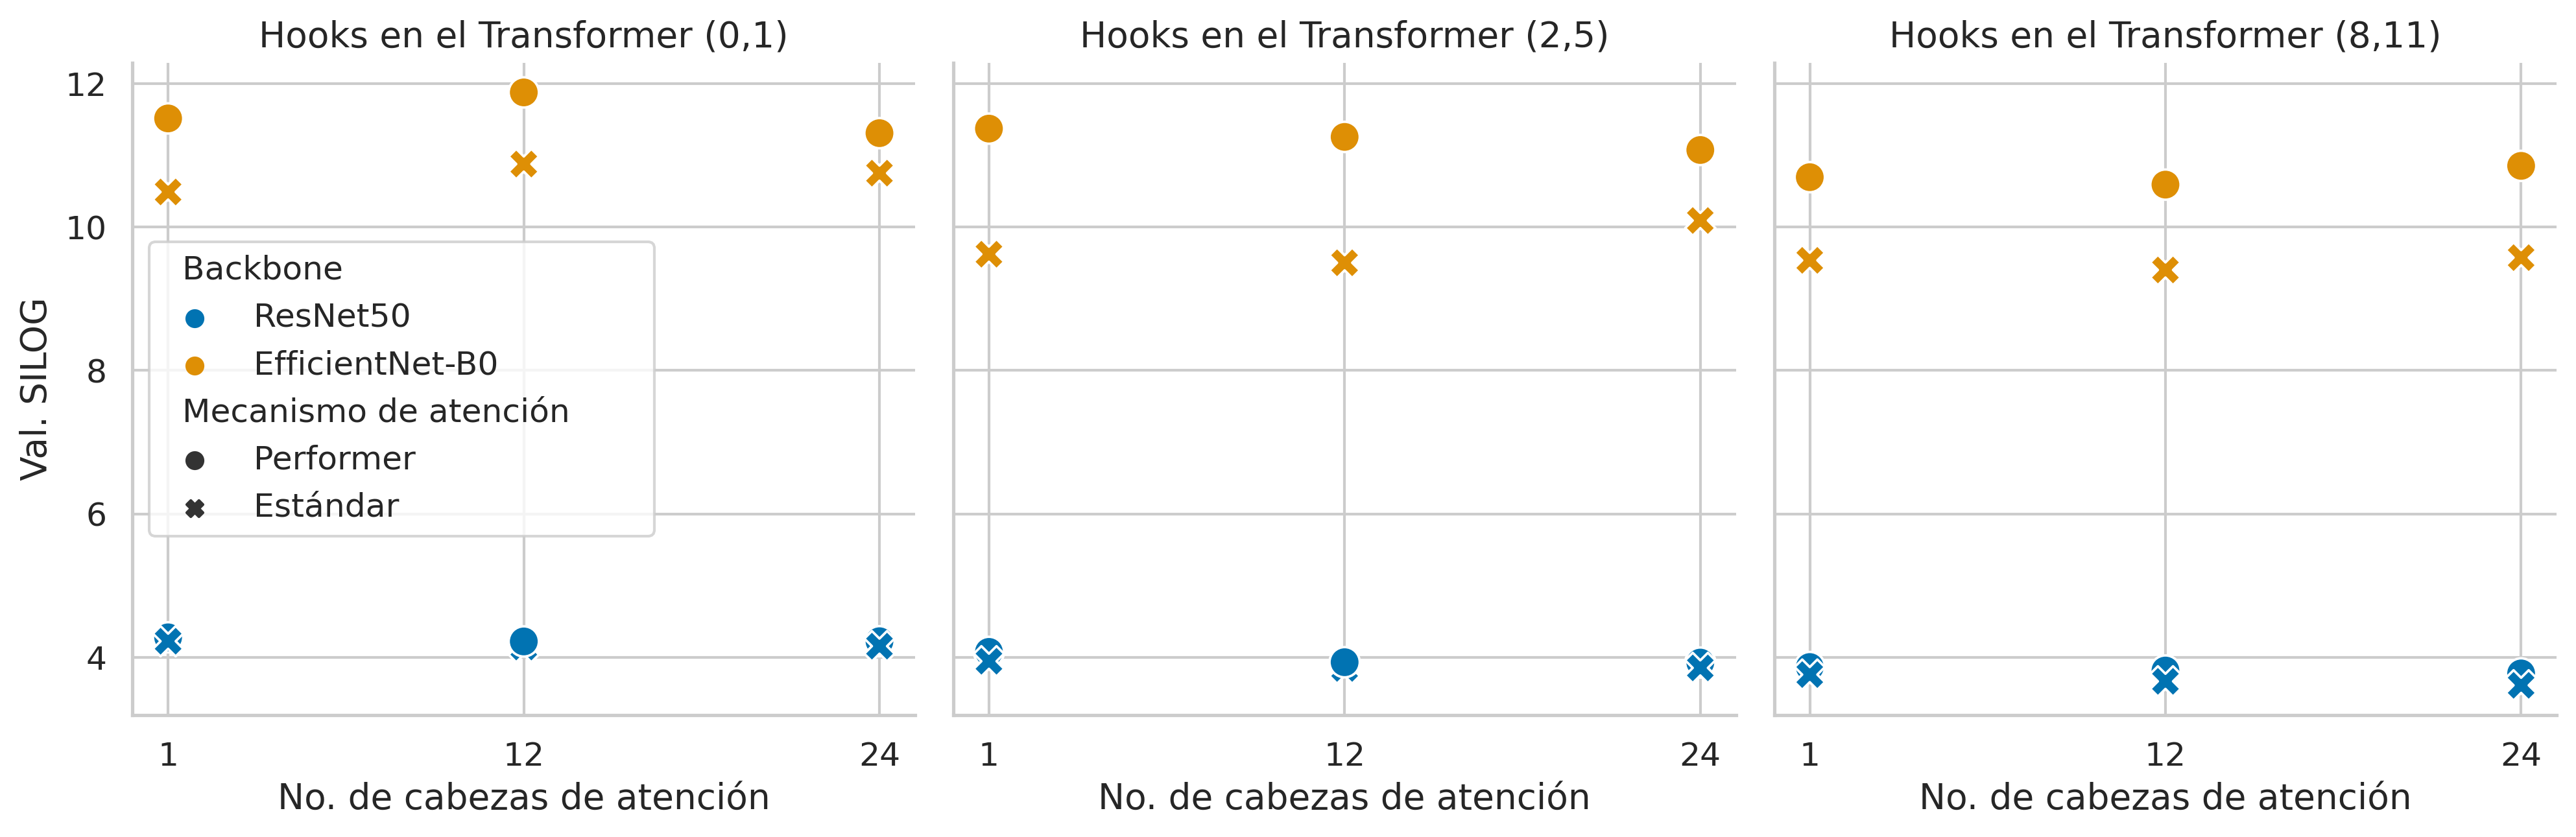
\includegraphics[width=\linewidth]{imagenes/Resultados/SIlog_val.png} 
\captionsetup{width=.95\linewidth}
\caption{SIlog obtenido en el conjunto de validación para cada uno de los 36 modelos entrenados. Más bajo es mejor.}
\label{fig:SIlog-validation}
\end{figure}

Con el objetivo de buscar la causa de esta diferencia tan grande del error, se estudian las curvas de aprendizaje de entrenamiento y validación. En estas curvas (\Cref{fig:efficientnet-overfitting}), se puede observar como en comparación con el modelo equivalente con ResNet50, el modelo que tiene como \textit{backbone} la EfficientNet-B0 está sobreajustado (\textit{overfitting}) sus parámetros al conjunto de entrenamiento, ya que la diferencia entre el error en el conjunto de entrenamiento y el error en el conjunto de validación es mucho mayor en el caso del modelo con EfficientNet.

\begin{figure}[H]
\centering
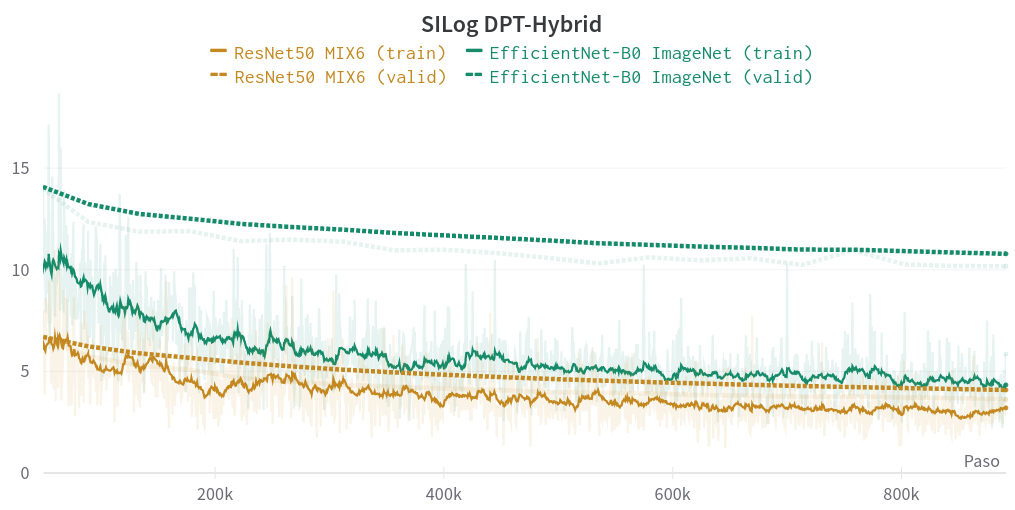
\includegraphics[width=\linewidth]{imagenes/Resultados/EfficientNet_overfitting.png} 
\captionsetup{width=.95\linewidth}
\caption{Comparación de las curvas de aprendizaje del SIlog durante el entrenamiento y validación de dos modelos con diferentes \textit{backbones} e inicializaciones de pesos. Valores suavizados con una media exponencial ponderada para facilitar su visualización.}
\label{fig:efficientnet-overfitting}
\end{figure}

Dado que los parámetros de EfficientNet-B0 se han inicializado con parámetros entrenados en ImageNet y no en MIX6 (\textit{dataset} de profundidad utilizado para preentrenar las ResNet50), se plantea un experimento adicional para descartar que esta falta de preentrenamiento especializado sea la causa del \textit{overfitting}. Para llevar a cabo este experimento, se extraen los parámetros de un ViT-Hybrid preentrenado en ImageNet y se utilizan para inicializar los pesos de un DPT-Hybrid con ResNet50. De esta forma, la ResNet50 parte de un estado similar al de la EfficientNet-B0 (preentrenamiento en ImageNet). En la \Cref{fig:mix6-imagenet}, se pueden apreciar los resultados en el conjunto de validación de estos tres modelos y se comprueba como el dominio del preentrenamiento no influye en el sobreajuste del \textit{backbone} convolucional.

\begin{figure}[H]
\centering
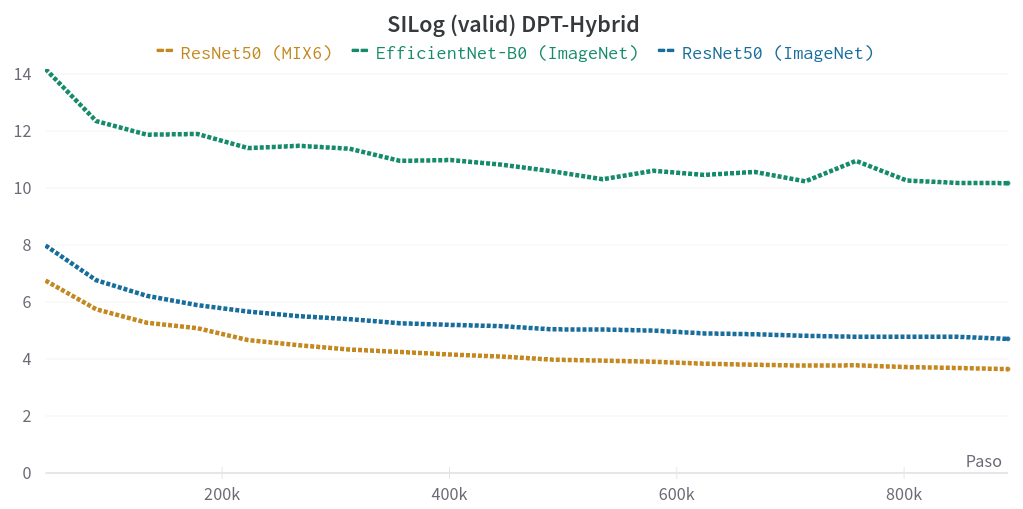
\includegraphics[width=\linewidth]{imagenes/Resultados/ResNet50ImageNet.png} 
\captionsetup{width=.95\linewidth}
\caption{Comparación del SIlog en el conjunto de validación durante el entrenamiento en tres modelos con diferentes inicializaciones de pesos.}
\label{fig:mix6-imagenet}
\end{figure}














































\subsection{Número de cabezas}\label{resultados-cuantitativos-cabezas}

En la \Cref{fig:SIlog-val-split}, equivalente a la \Cref{fig:SIlog-validation} pero separada en función del \textit{backbone}, es posible ver como la diferencia en los resultados según el número de cabezas en los bloques de atención es relativamente pequeña, especialmente en el caso del mecanismo de atención estándar.

\begin{figure}[H]
\centering
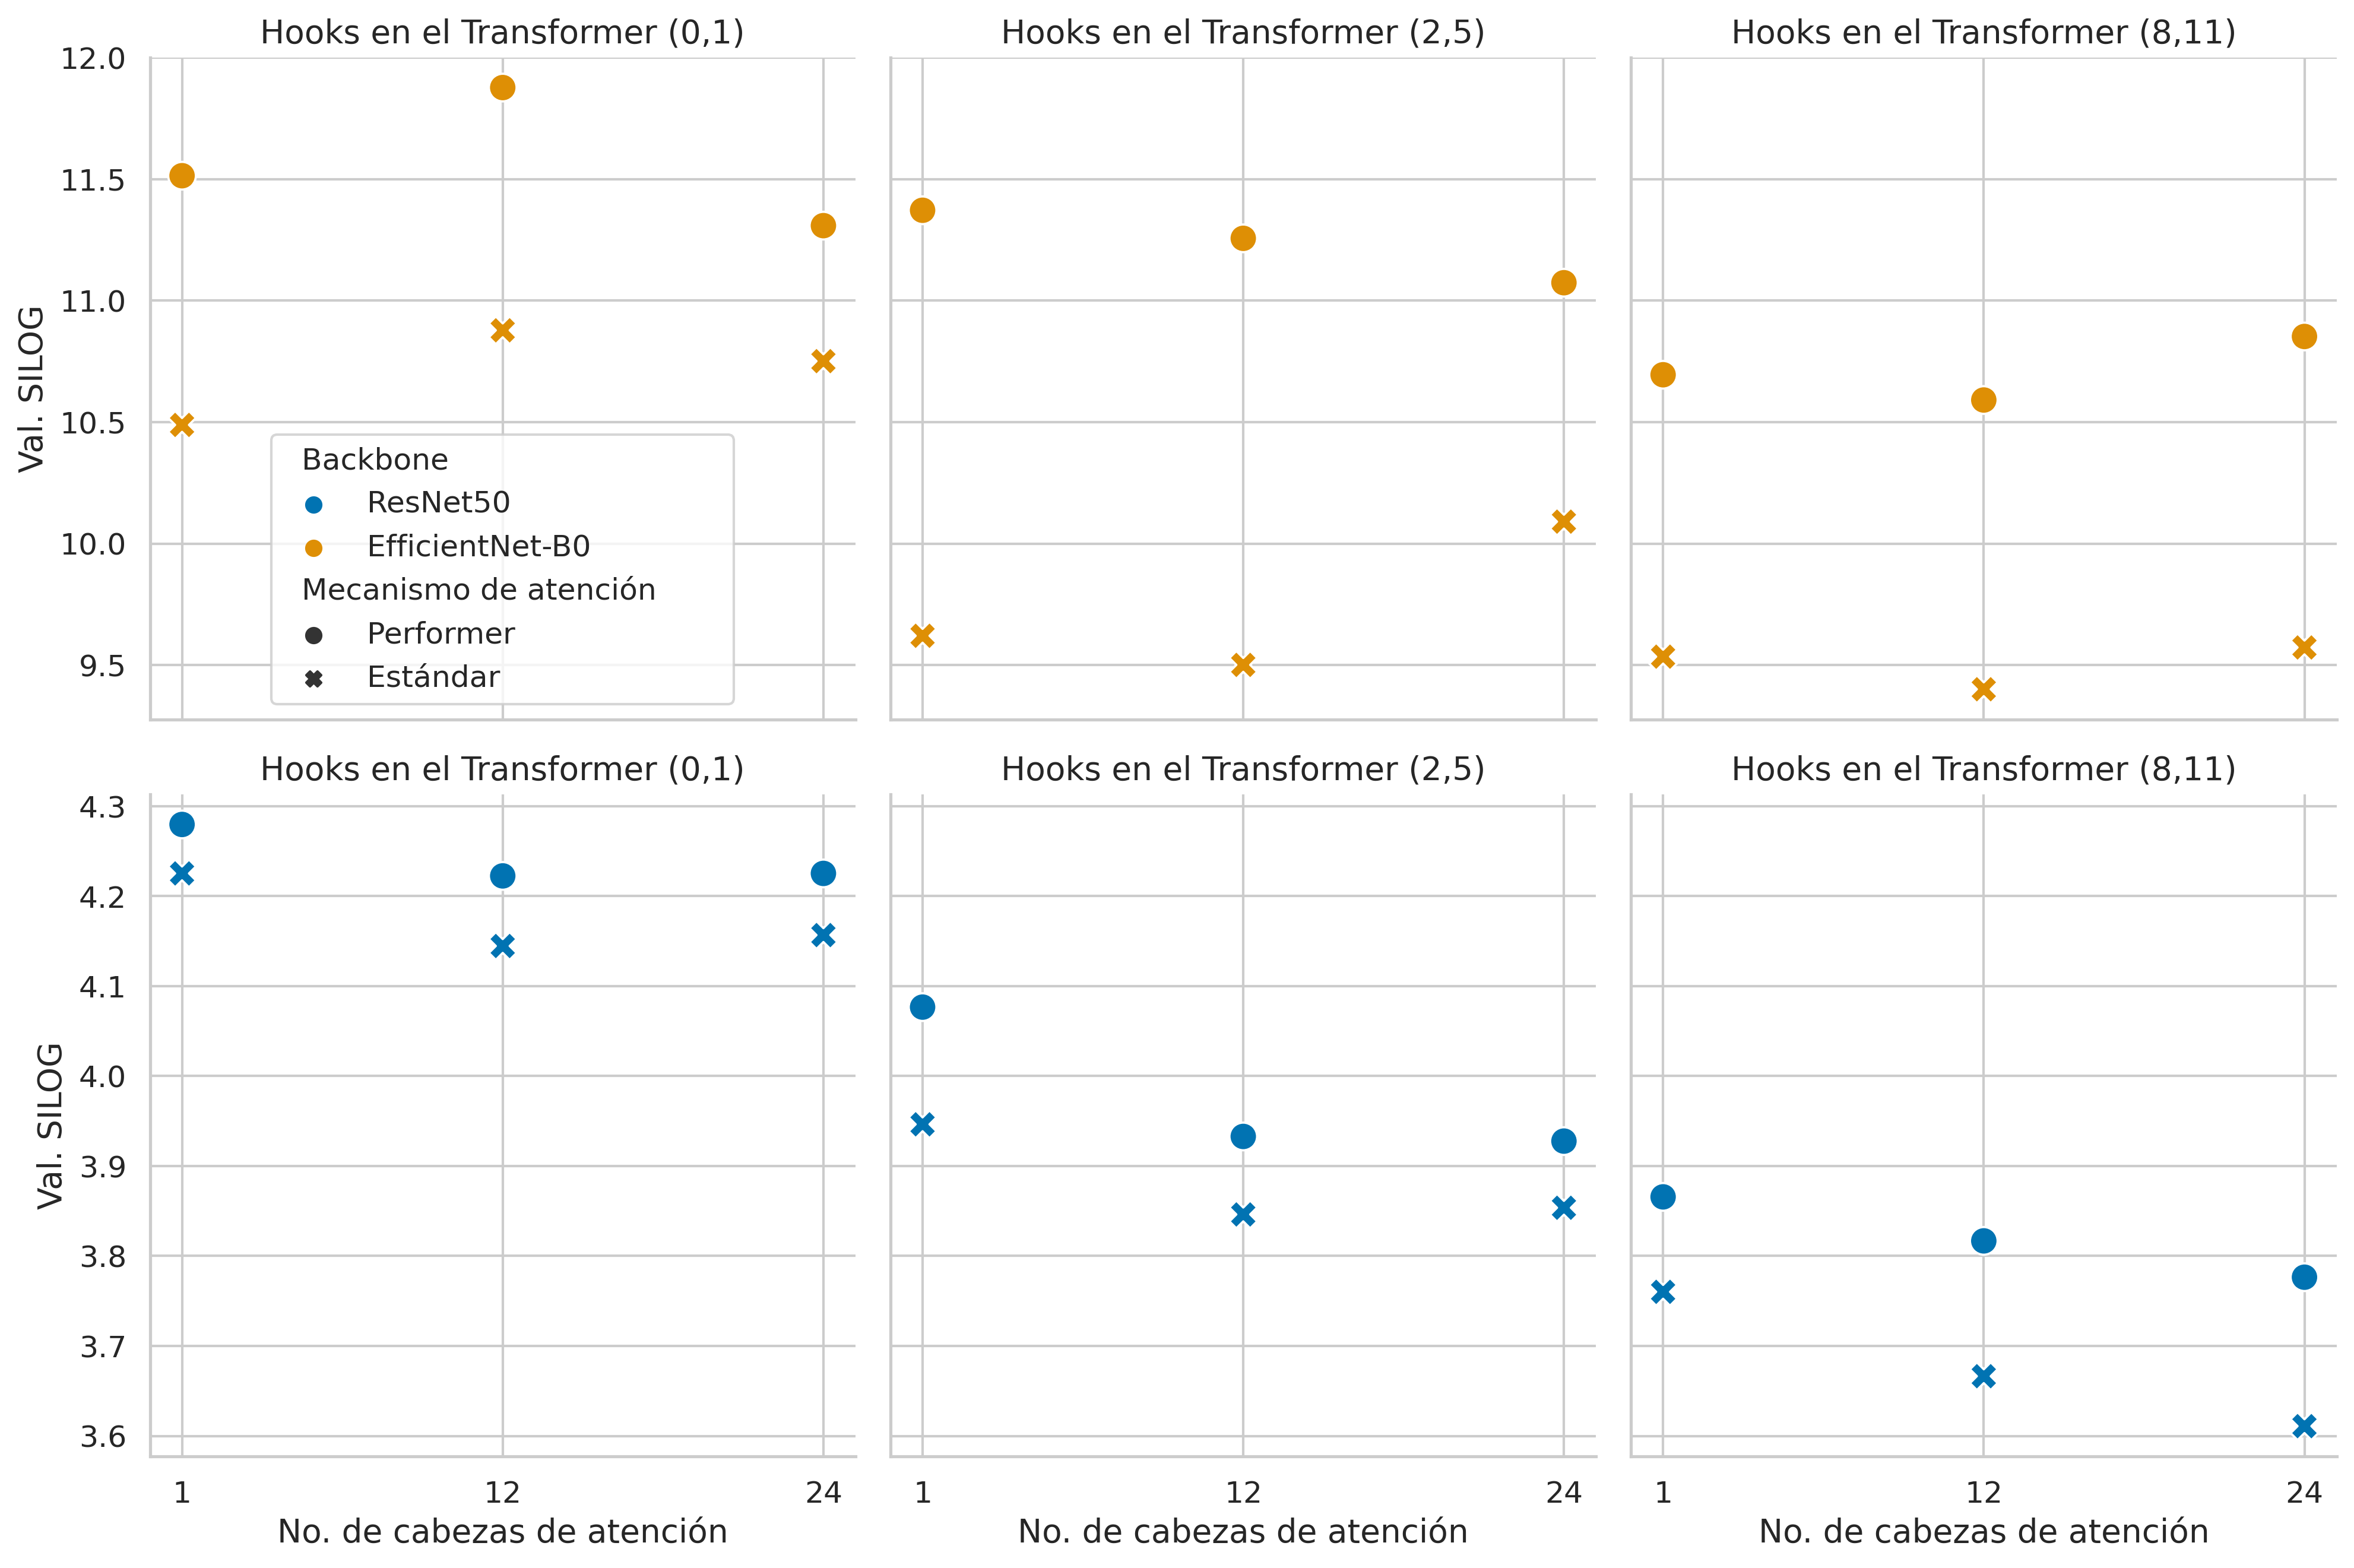
\includegraphics[width=\linewidth]{imagenes/Resultados/SIlog_val_split.png} 
\captionsetup{width=.95\linewidth}
\caption{SIlog obtenido en el conjunto de validación para cada uno de los 36 modelos entrenados con distintos ejes en función del \textit{backbone}. Más bajo es mejor.}
\label{fig:SIlog-val-split}
\end{figure}

De forma similar, en el caso de las métricas de velocidad de inferencia (\Cref{fig:resultados-inf-num-cabezas}), sobretodo en el caso de las imágenes reducidas, no se encuentra un aumento de la velocidad especialmente significativo.

\begin{figure}[H]
\centering
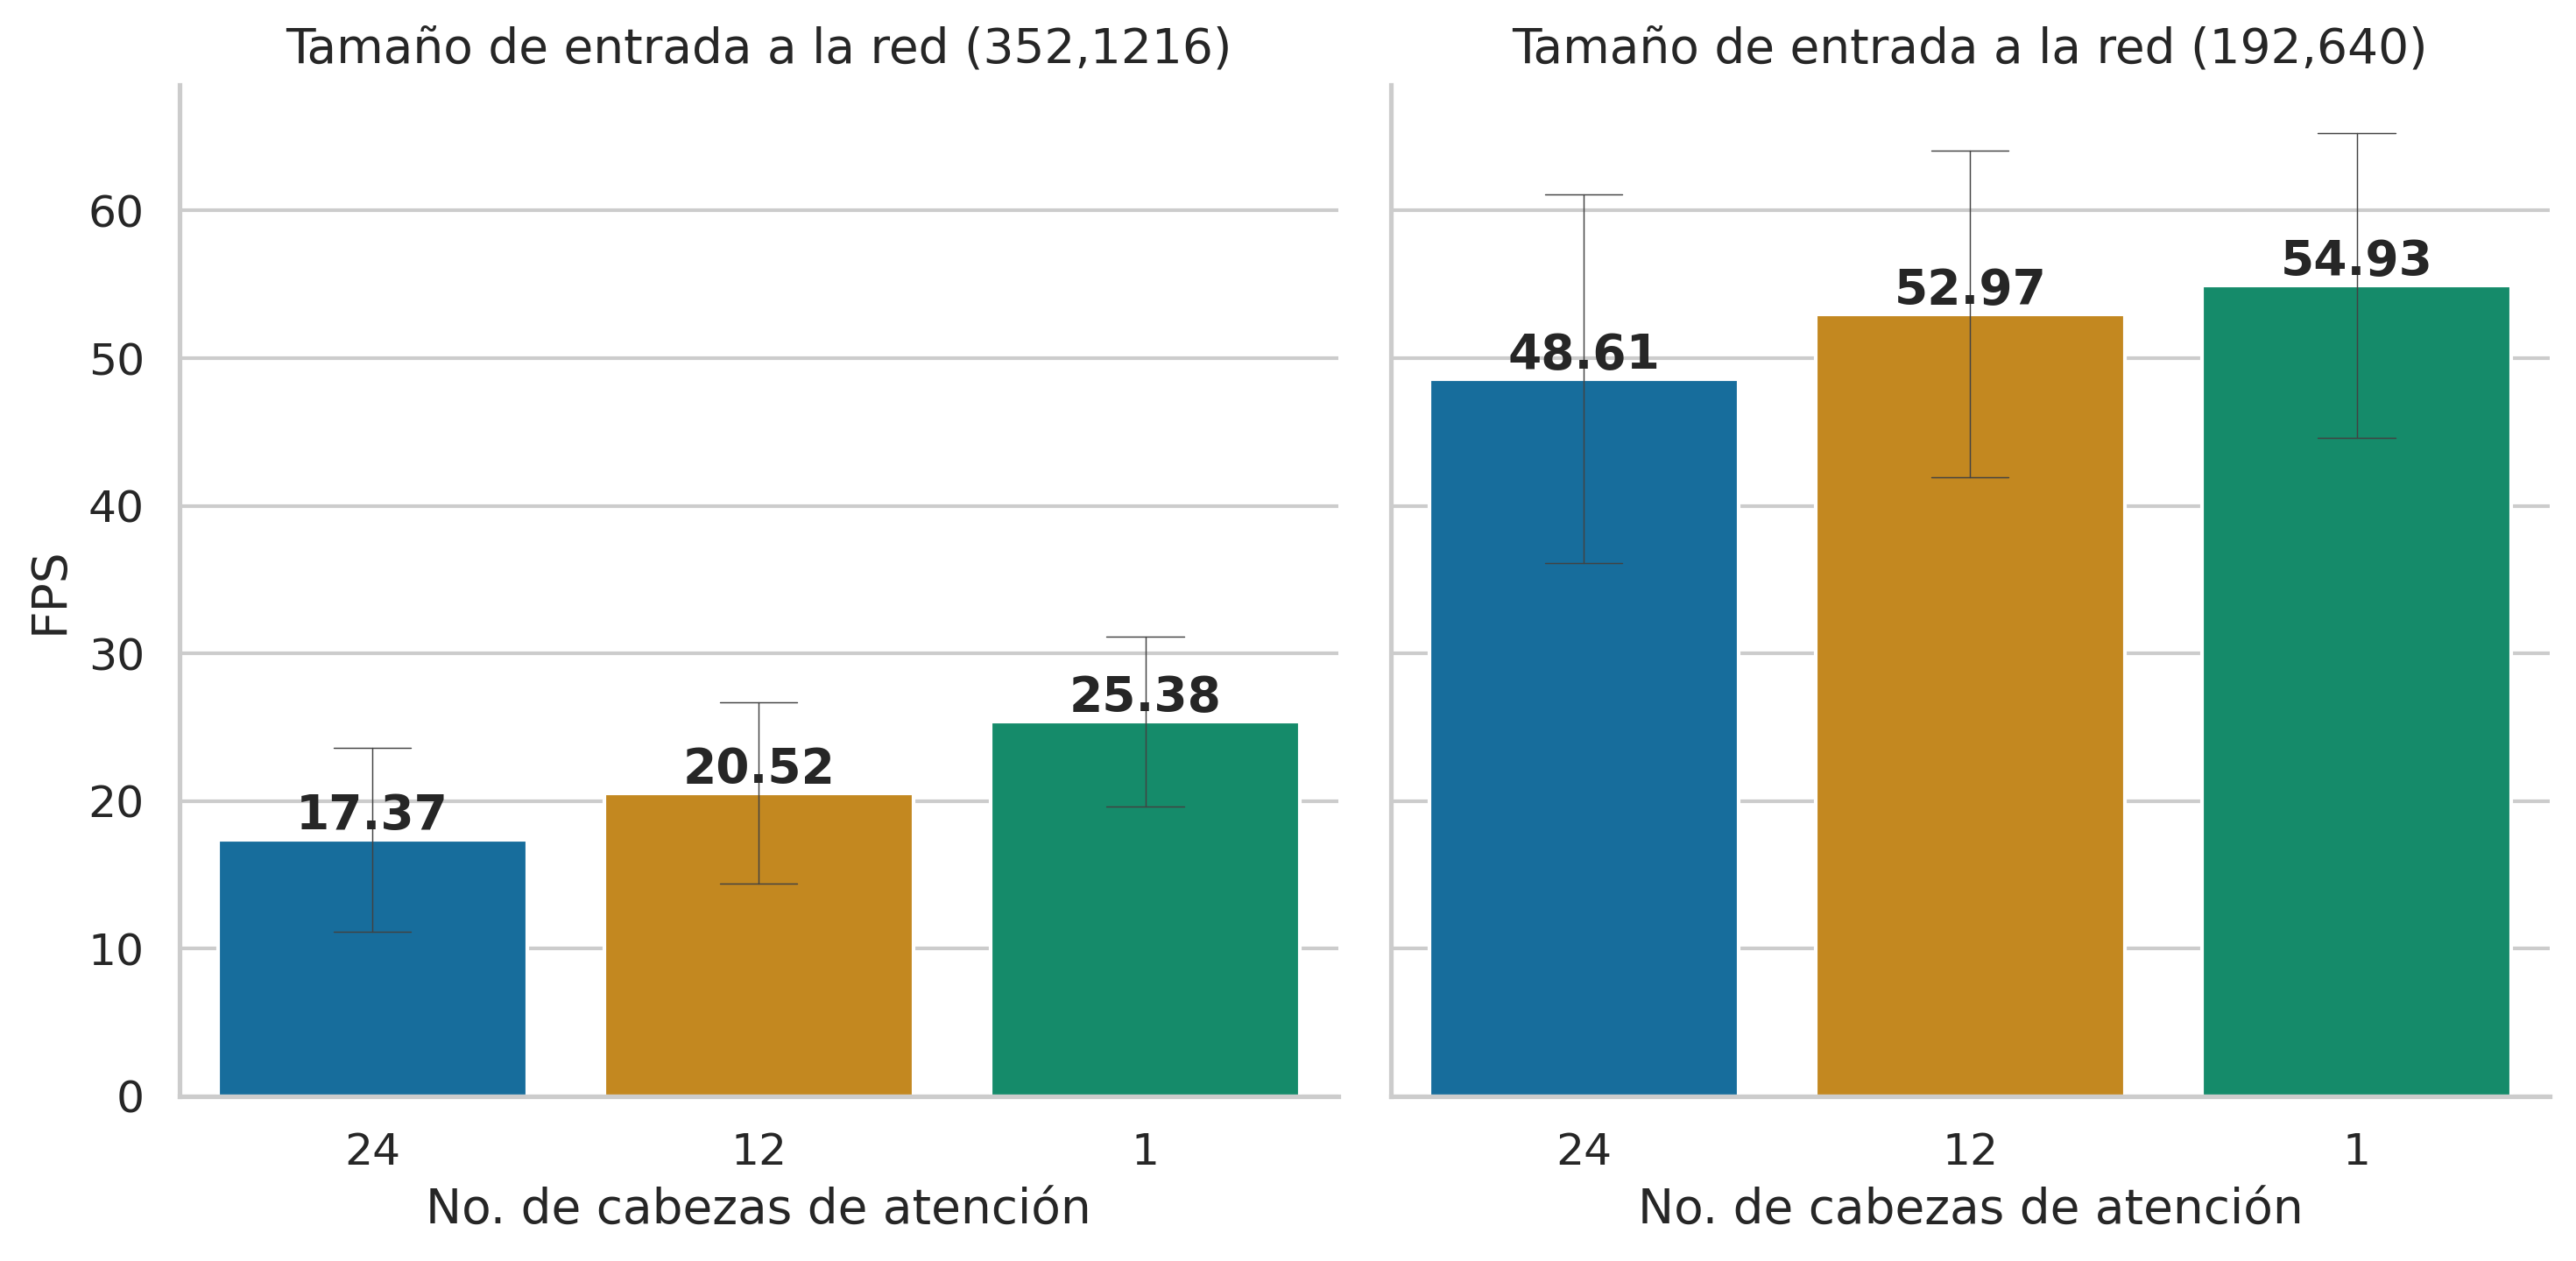
\includegraphics[width=0.75\linewidth]{imagenes/Resultados/velocidad_inferencia_cabezas_atencion.png} 
\captionsetup{width=.8\linewidth}
\caption{FPS medios de los modelos en función del número de cabezas utilizado y del tamaño de la entrada. Las barras grises representan la desviación estándar de las medidas.}
\label{fig:resultados-inf-num-cabezas}
\end{figure}
























\subsection{Capas de atención eficiente}\label{resultados-cuantitativos-atencion}
Tal y como se ha visto en la \Cref{fig:SIlog-val-split}, el cambio del mecanismo de atención eficiente también influye negativamente en la calidad de los resultados. Dado que el incremento de la métrica de error es relativamente pequeño, esto podría ser totalmente aceptable si no fuese por los resultados de las métricas de velocidad (\Cref{fig:resultados-inf-mec-atention}), donde se puede observar que los modelos con el mecanismo de atención eficiente (\textit{Performer}) son en realidad más lentos cuando el tamaño de la entrada es reducido.

\begin{figure}[H]
\centering
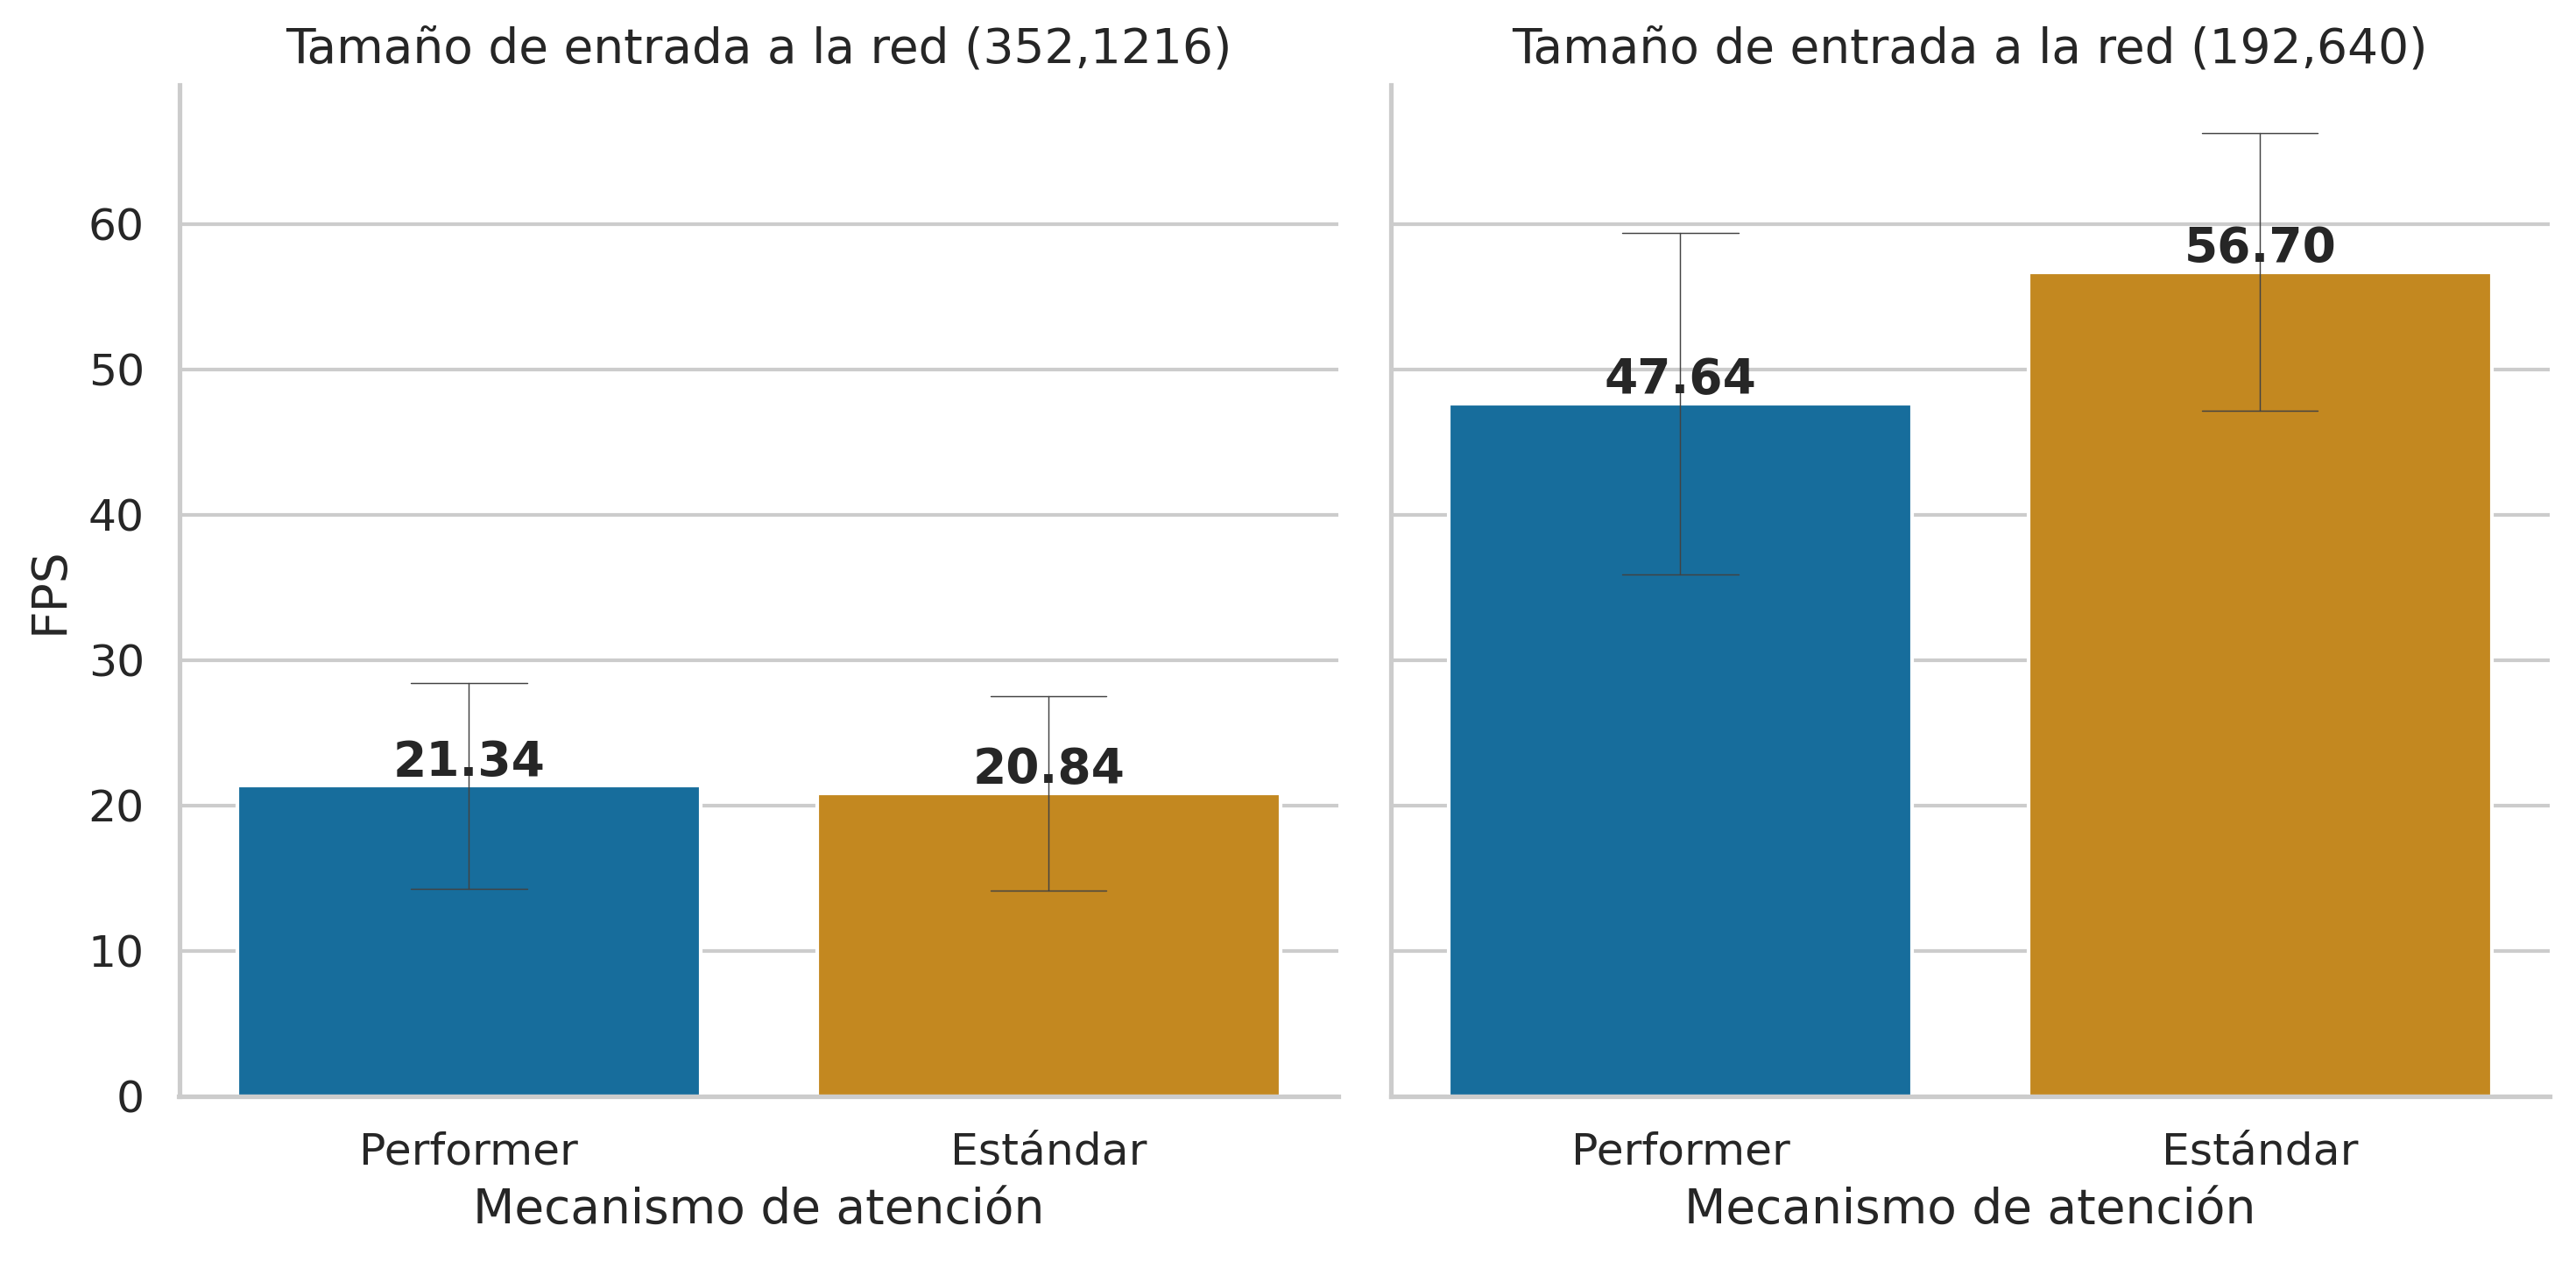
\includegraphics[width=0.9\linewidth]{imagenes/Resultados/velocidad_inferencia_mecanismo_atencion.png} 
\captionsetup{width=.9\linewidth}
\caption{FPS medios de los modelos en función del mecanismo de atención utilizado y del tamaño de la entrada. Las barras grises representan la desviación estándar de las medidas.}
\label{fig:resultados-inf-mec-atention}
\end{figure}

Esto, se debe a que, pese a que la complejidad del mecanismo de atención eficiente es $O(n)$ y la del mecanismo de atención estándar es $O(n^2)$, existe un \textit{overhead} asociado al mecanismo de atención eficiente que hace que la ejecución para secuencia de elementos cortas (como es el caso de la imagen reducida) sea más lento que con la atención estándar. En la \Cref{fig:resultados-complejidad-mec-atencion}, donde se muestran los resultados de otro experimento donde se incrementó la longitud de la secuencia de entrada progresivamente para medir el tiempo de inferencia de un bloque de atención, se puede apreciar este comportamiento.

\begin{figure}[H]
\centering
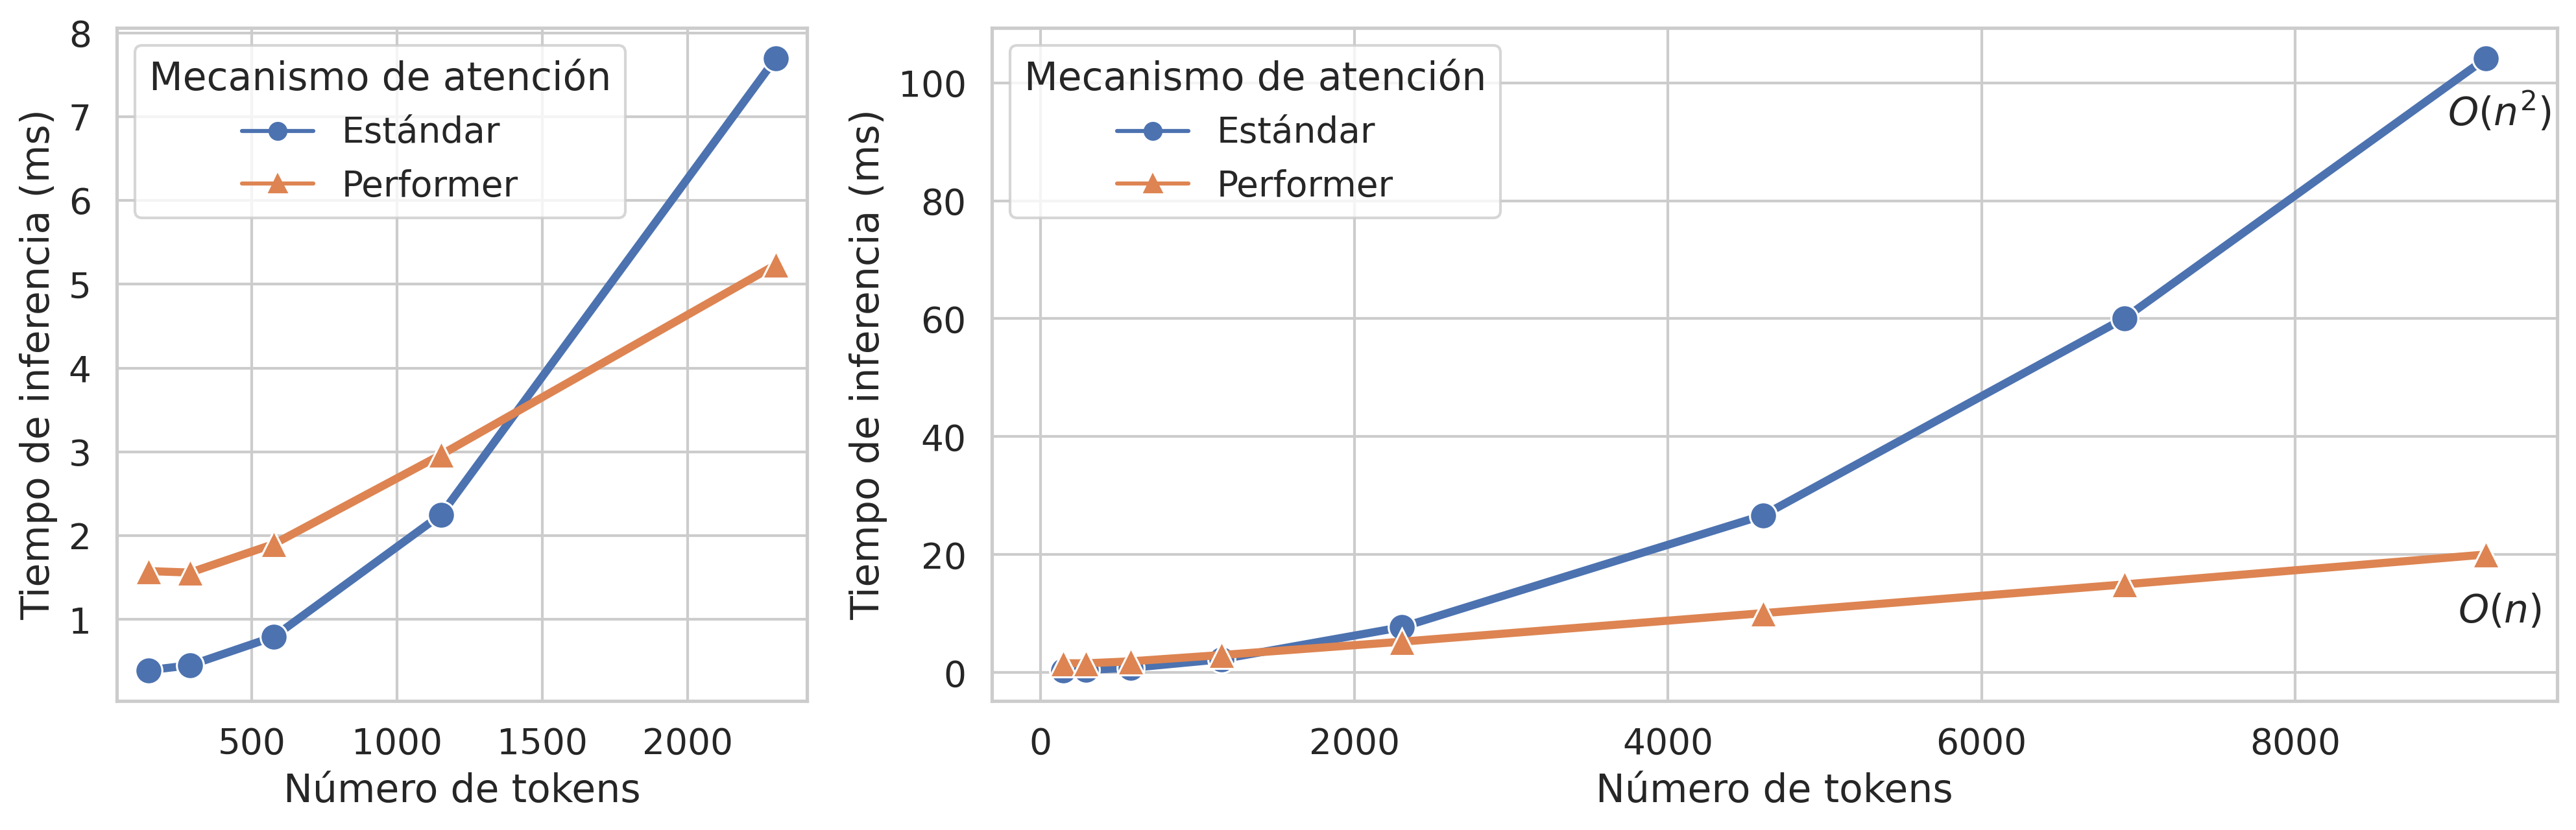
\includegraphics[width=\linewidth]{imagenes/Resultados/complejidad_mecanismo_atencion.png} 
\captionsetup{width=.95\linewidth}
\caption{Comparación de la complejidad y el tiempo de inferencia en un bloque de atención usando el mecanismo de atención estándar y el mecanismo eficiente del \textit{Performer}. Detalle de los tiempos de inferencia para entradas con un número de \textit{tokens} reducido a la izquierda.}
\label{fig:resultados-complejidad-mec-atencion}
\end{figure}

















\subsection{Cambio en los hooks del transformer y eliminación de las capas de atención posteriores}\label{resultados-cuantitativos-hooks}
La última modificación de la arquitectura estudiada, el cambio en los \textit{hooks}, es decir, la elección de los bloques de atención de los cuales se toman las salidas como entradas del \textit{encoder} es, después del cambio de \textit{backbone}, la que más afecta a la calidad de los resultados (\Cref{fig:SIlog-val-split}). Por otro lado, el incremento en la velocidad de inferencia asociado a este cambio sí que es considerable (\Cref{fig:resultados-inf-hooks}) llegando casi a duplicar los FPS en los modelos con la entrada a resolución original y aumentando en más de un $50\%$ los FPS cuando el tamaño de la entrada se ha reducido.

\begin{figure}[H]
\centering
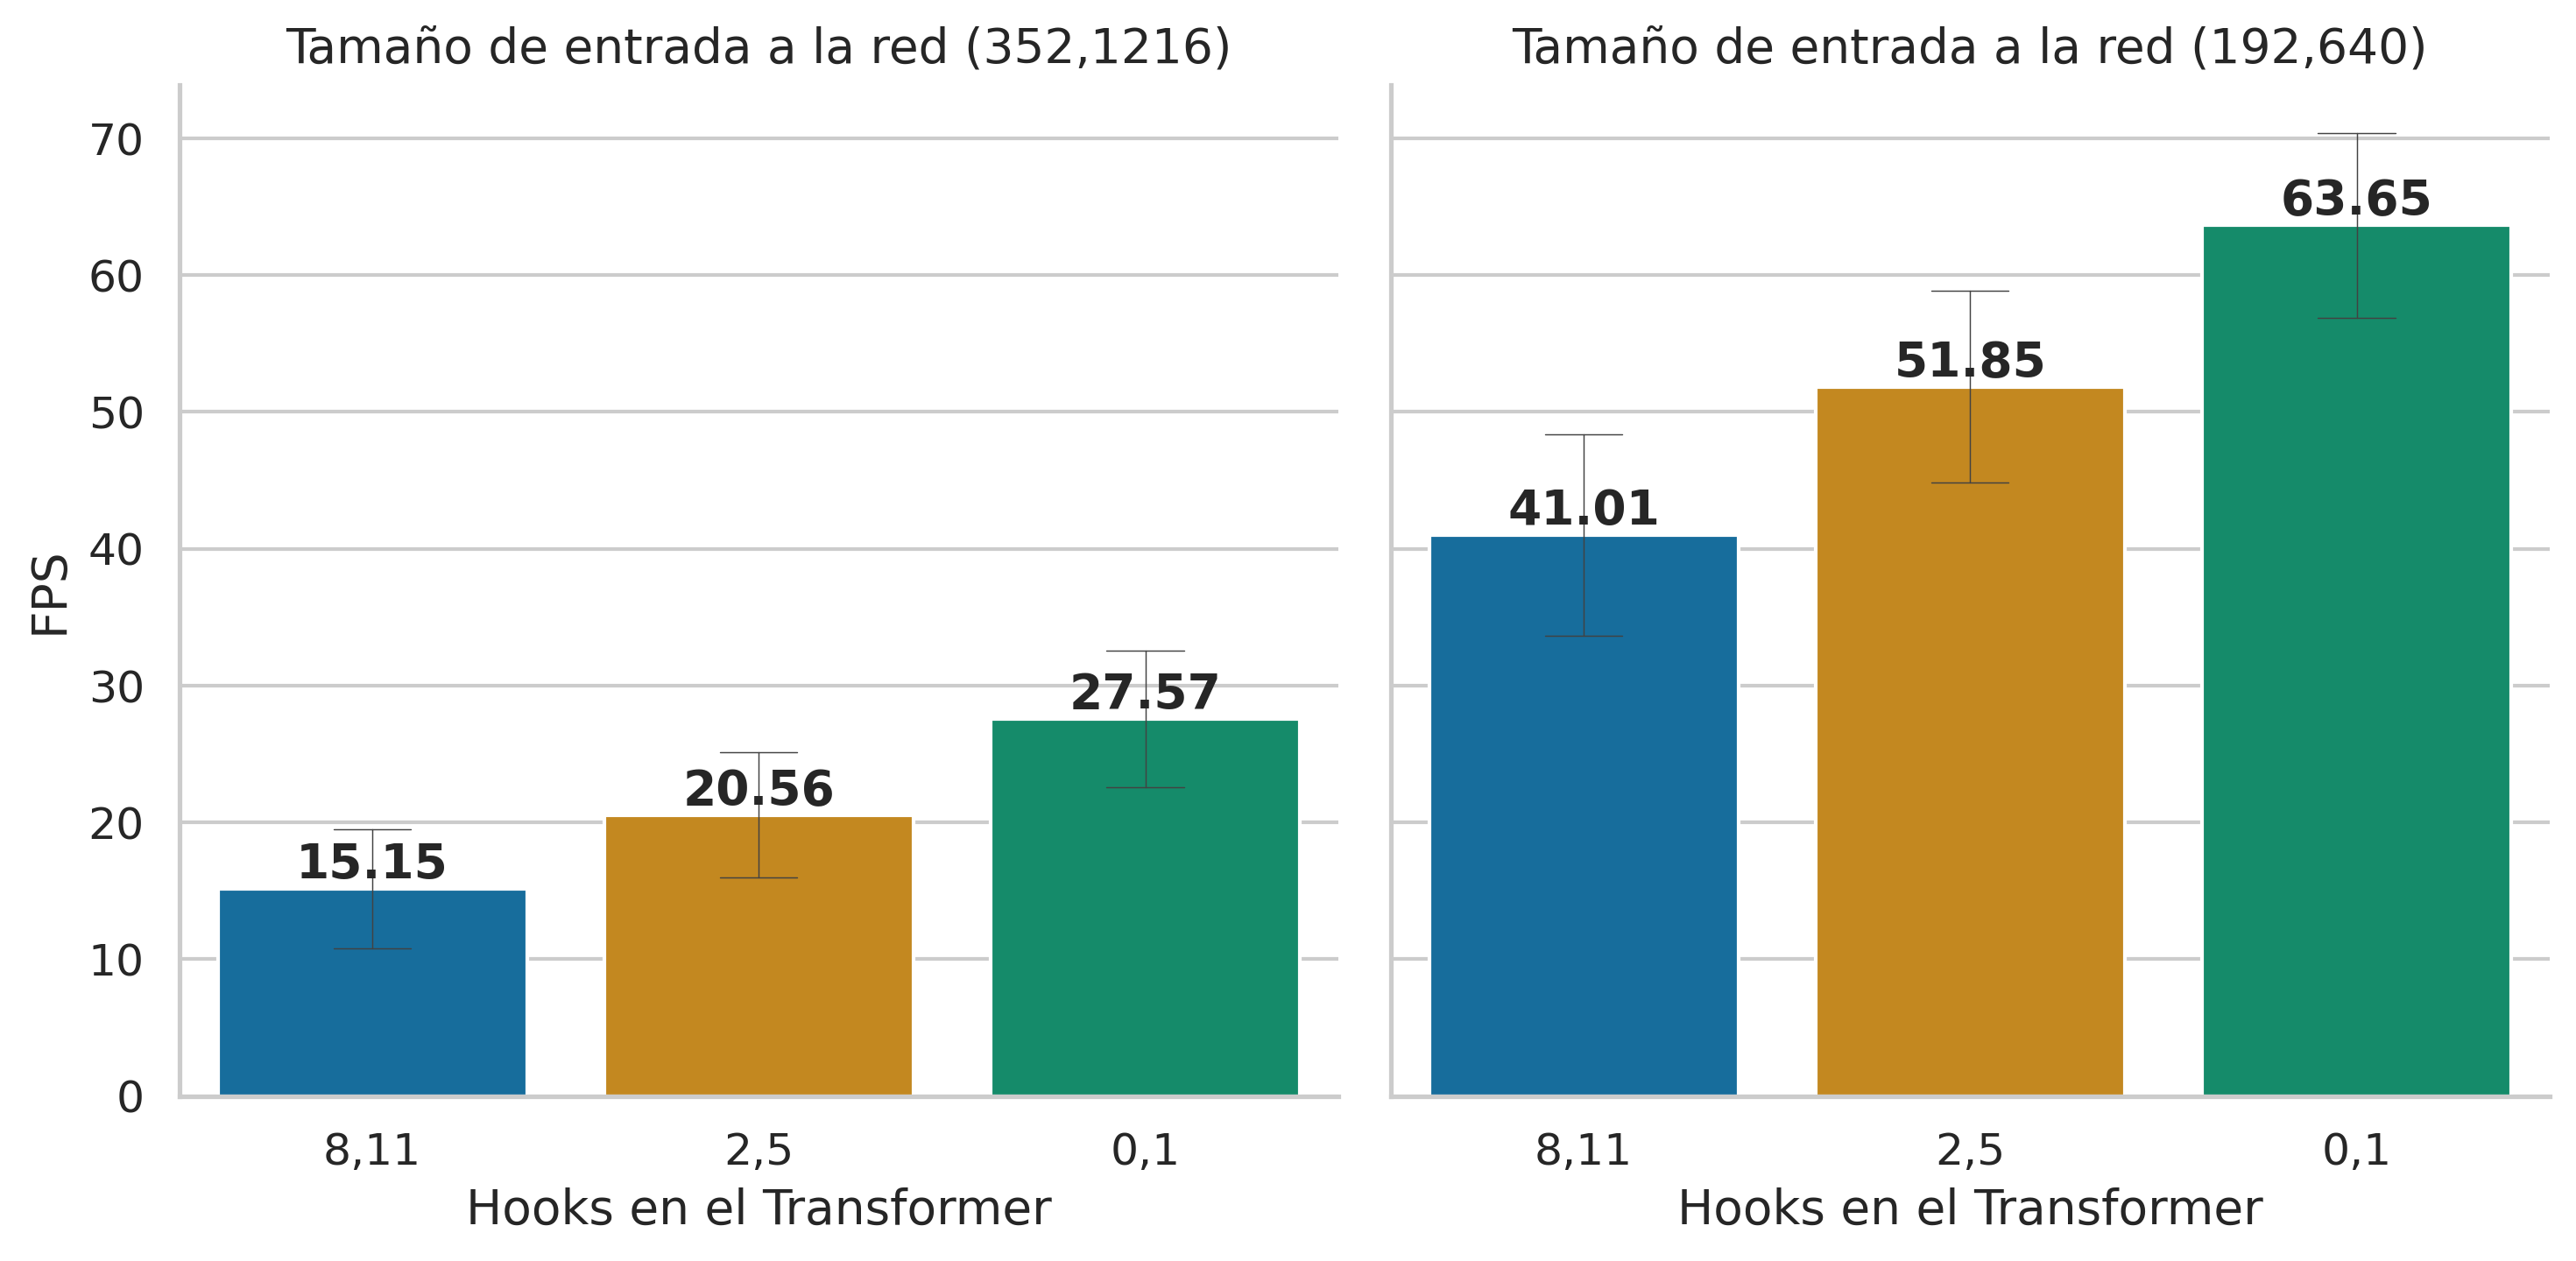
\includegraphics[width=0.85\linewidth]{imagenes/Resultados/velocidad_inferencia_hooks.png} 
\captionsetup{width=.9\linewidth}
\caption{FPS medios de los modelos en función de los \textit{hooks} utilizados y del tamaño de la entrada. Las barras grises representan la desviación estándar de las medidas.}
\label{fig:resultados-inf-hooks}
\end{figure}















\section{Tamaño de los modelos y número de operaciones}
El tamaño de los modelos también se ve afectado por las modificaciones del modelo que se han llevado a cabo en este proyecto. En la \Cref{fig:resultados-mb} se puede ver el tamaño en \textit{megabytes} (MB) que ocupan los modelos. En esta gráfica, puede apreciarse como la mayor diferencia viene dada por los bloques donde se situan los \textit{hooks} ya que al elegir los bloques iniciales del \textit{transformer} es posible eliminar todos los parámetros correspondientes a los bloques de atención posteriores. Cabe destacar también de estos resultados cómo la diferencia de tamaño entre los modelos en función del \textit{backbone} convolucional es relativamente pequeña, y la forma en que el número de cabezas afecta al tamaño del modelo en función del mecanismo de atención empleado.


\begin{figure}[H]
\centering
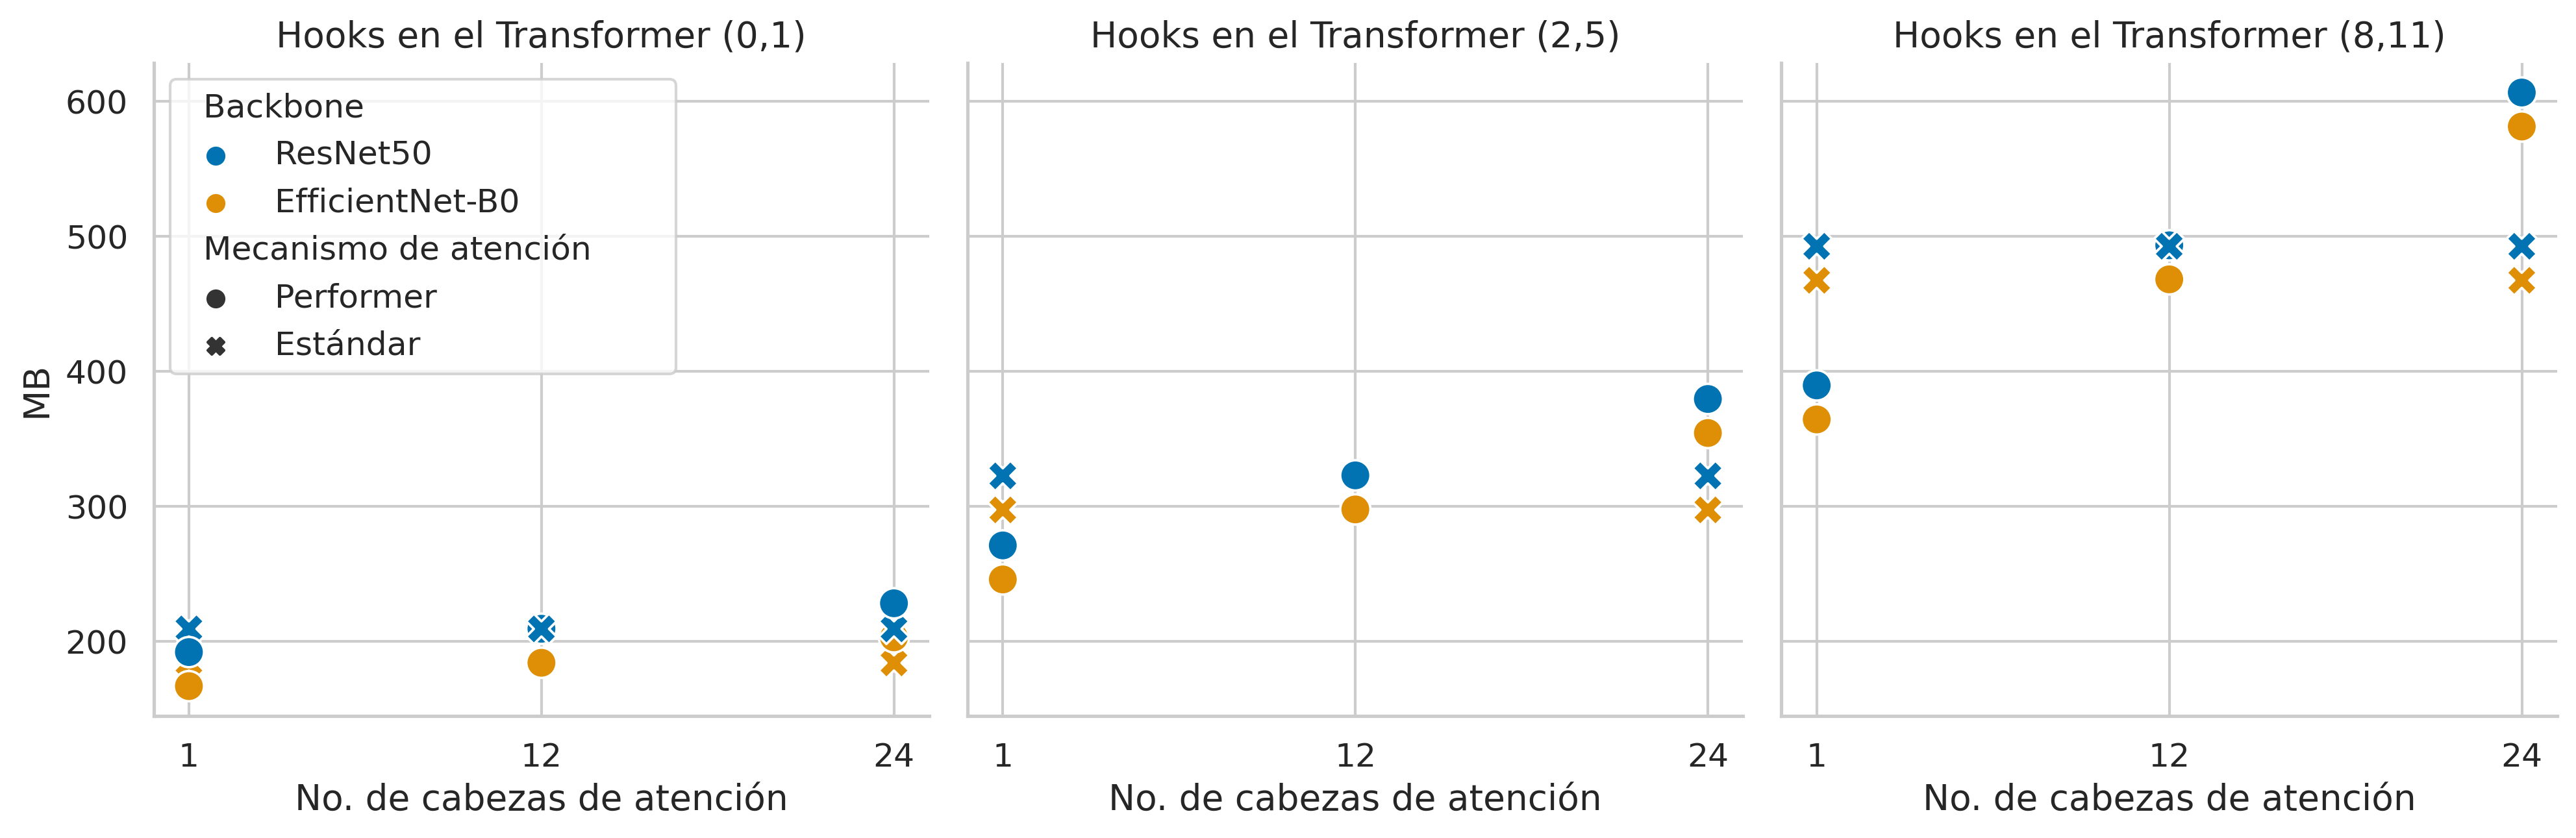
\includegraphics[width=\linewidth]{imagenes/Resultados/mb.png} 
\captionsetup{width=0.95\linewidth}
\caption{Tamaño en memoria de los modelos en función de su configuración.}
\label{fig:resultados-mb}
\end{figure}

La tendencia de los tamaños de los modelos en función de sus características es posible verla también en las medidas de Giga FLOPs (número de operaciones en coma flotante requeridas para inferir la salida con una sola entrada) presentadas en la \Cref{fig:resultados-gflops}. No obstante, una diferencia interesante entre estas dos Figuras es que en el número de operaciones necesarias para obtener la salida del modelo sí que influye en mayor medida la elección del \textit{backbone} convolucional, es decir, se puede comprobar que para un número de parámetros similar, EfficientNet-B0 lleva a cabo un número de operaciones menor que ResNet50.

\begin{figure}[H]
\centering
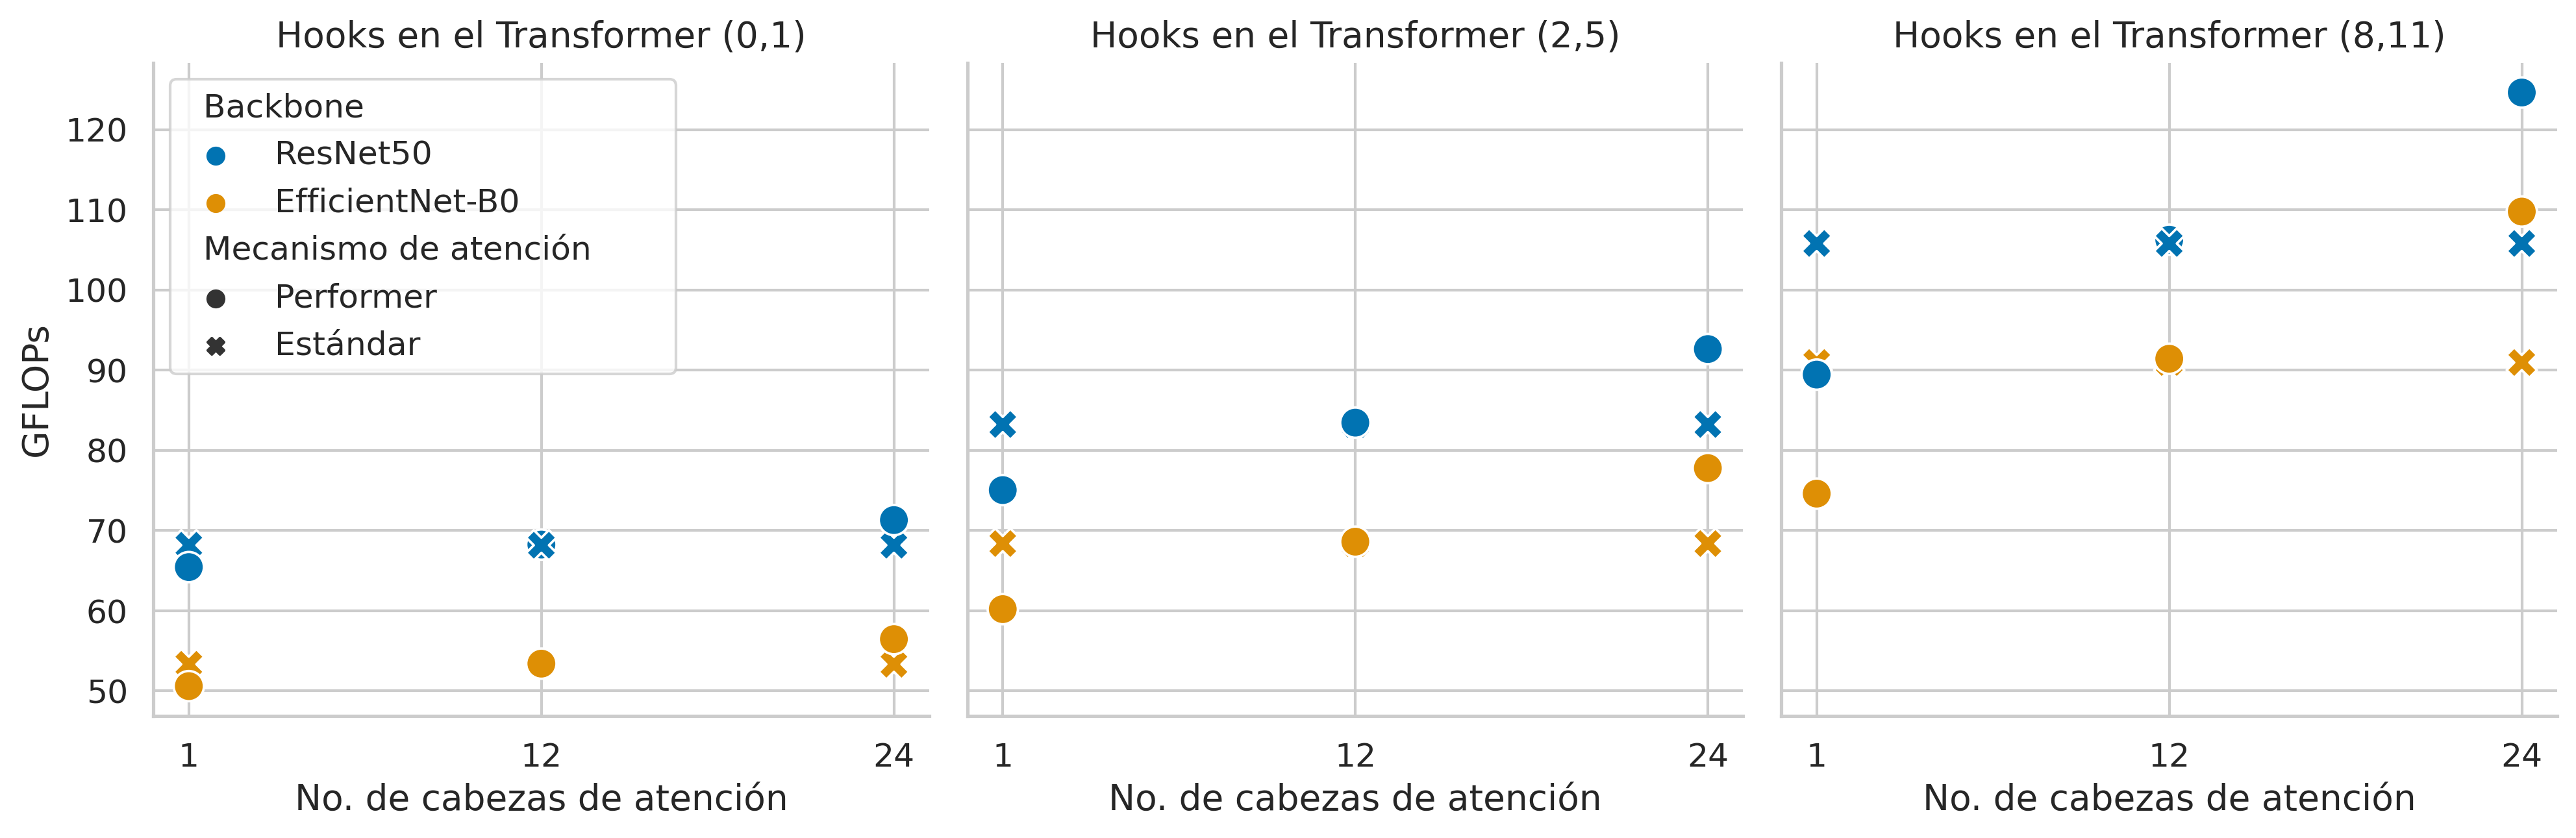
\includegraphics[width=\linewidth]{imagenes/Resultados/gflops.png} 
\captionsetup{width=.95\linewidth}
\caption{Número de operaciones en coma flotante necesarias para inferir la profundidad en una imagen en función de la configuración del modelo.}
\label{fig:resultados-gflops}
\end{figure}















\section{Resultados cualitativos}

En esta sección, se presentan los resultados en el conjunto de evaluación (\textit{test}) de distintos modelos en función de sus modificaciones, con el objetivo de comparar visualmente y apreciar las diferencias entre las salidas que generan las distintas arquitecturas. Las imágenes generadas los valores solo ocupan una pequeña parte de la escala de grises, sin embargo, las imágenes siguientes han sido escaladas para ocupar todo el rango de grises, facilitando así la apreciación de detalles. 

%% http://www.peteryu.ca/tutorials/publishing/latex_captions_old
%% https://tex.stackexchange.com/questions/162824/vertical-spacing-between-subfloat
%% https://tex.stackexchange.com/questions/395515/how-to-scale-and-align-figures-and-tables-in-latex-in-a-3x2-grid-like-manner




%\captionsetup[subfigure]{labelformat=empty}
%    \begin{figure}[!ht]
%\centering
%    \subfloat{\includegraphics[width=0.33\linewidth]{imagenes/test_output_samples/input/2011_09_26_drive_0002_sync_0000000021.png}}
%\hfil
%    \subfloat{
\includegraphics[width=0.33\linewidth]{imagenes/test_output_samples/2011_09_26_drive_0002_sync_0000000021/e7069aae.png}}
%\hfil
%    \subfloat{\includegraphics[width=0.33\linewidth]{imagenes/test_output_samples/2011_09_26_drive_0002_sync_0000000021/qsudwuyk.png}}\\[-2ex]
%
%
%    \subfloat{\includegraphics[width=0.33\linewidth]{imagenes/test_output_samples/input/2011_09_26_drive_0009_sync_0000000112.png}}
%\hfil
%    \subfloat{
\includegraphics[width=0.33\linewidth]{imagenes/test_output_samples/2011_09_26_drive_0009_sync_0000000112/e7069aae.png}}
%\hfil
%    \subfloat{\includegraphics[width=0.33\linewidth]{imagenes/test_output_samples/2011_09_26_drive_0009_sync_0000000112/qsudwuyk.png}}\\[-2ex]
%    
%    
%    \subfloat{\includegraphics[width=0.33\linewidth]{imagenes/test_output_samples/input/2011_09_26_drive_0009_sync_0000000196.png}}
%\hfil
%    \subfloat{
\includegraphics[width=0.33\linewidth]{imagenes/test_output_samples/2011_09_26_drive_0009_sync_0000000196/e7069aae.png}}
%\hfil
%    \subfloat{\includegraphics[width=0.33\linewidth]{imagenes/test_output_samples/2011_09_26_drive_0009_sync_0000000196/qsudwuyk.png}}\\[-2ex]
%    
%    
%    
%    \subfloat{\includegraphics[width=0.33\linewidth]{imagenes/test_output_samples/input/2011_09_26_drive_0009_sync_0000000292.png}}
%\hfil
%    \subfloat{
\includegraphics[width=0.33\linewidth]{imagenes/test_output_samples/2011_09_26_drive_0009_sync_0000000292/e7069aae.png}}
%\hfil
%    \subfloat{\includegraphics[width=0.33\linewidth]{imagenes/test_output_samples/2011_09_26_drive_0009_sync_0000000292/qsudwuyk.png}}\\[-2ex]
%    
%    
%    
%    \subfloat{\includegraphics[width=0.33\linewidth]{imagenes/test_output_samples/input/2011_09_26_drive_0009_sync_0000000324.png}}
%\hfil
%    \subfloat{\includegraphics[width=0.33\linewidth]{imagenes/test_output_samples/2011_09_26_drive_0009_sync_0000000324/e7069aae.png}}
%\hfil
%    \subfloat{\includegraphics[width=0.33\linewidth]{imagenes/test_output_samples/2011_09_26_drive_0009_sync_0000000324/qsudwuyk.png}}\\[-2ex]
%
%
%
%    \subfloat[Entrada]{\includegraphics[width=0.33\linewidth]{imagenes/test_output_samples/input/2011_09_26_drive_0013_sync_0000000030.png}}
%\hfil
%    \subfloat[Salida DPT sin modificar]{\includegraphics[width=0.33\linewidth]{imagenes/test_output_samples/2011_09_26_drive_0013_sync_0000000030/e7069aae.png}}
%\hfil
%    \subfloat[Salida DPT modificado]{\includegraphics[width=0.33\linewidth]{imagenes/test_output_samples/2011_09_26_drive_0013_sync_0000000030/qsudwuyk.png}}
%    
%\caption{Comparación cualitativa de resultados en el conjunto de evaluación entre el modelo DPT original y el modelo DPT con las modificaciones desarrolladas en este trabajo. Para facilitar su visualización, el rango de las profundidades predichas se ha ajustado a toda la escala de grises.}
%    \label{fig:comparacion-cualitativa}
%    \end{figure}
%\captionsetup[subfigure]{labelformat=parens}





En la primera comparación de resultados (\Cref{fig:cualitativa-1}), se encuentran las salidas del modelo original DPT-Hybrid publicado en \cite{visiontransformersDPT} y el modelo equivalente entrenado durante este trabajo. Es decir, la diferencia entre los dos modelos es el tamaño de las imágenes con las que se ha entrenado y el \textit{script} de entrenamiento empleado (como recordatorio, la imagen se reduce antes de ser procesada, pero después se vuelve a escalar a su tamaño original en la salida). En cuanto a las dos salidas, si bien es cierto que en la salida correspondiente a la entrada reducida (c) se pueden apreciar unos bordes menos suavizados, también es posible observar como la salida es considerablemente similar.

Por otro lado, en la \Cref{fig:cualitativa-2}, donde se comparan las salidas del modelo original entrenado con imágenes reducidas y el modelo equivalente pero con EfficientNet-B0 como \textit{backbone}, sí que se puede observar un deterioro de los resultados que se corresponde con la diferencia en las métricas del \Cref{resultados-cuantitativos-backbone}, por ejemplo, en el pilar del puente mostrado en el detalle.

\pagebreak

\captionsetup[subfigure]{labelformat=empty}
\begin{figure}[!ht]
\centering

    \subfloat{\bottominset{\colorbox{white}{\textbf{(a)}}}{\includegraphics[width=0.66\linewidth]{imagenes/test_output_samples/input/2011_09_26_drive_0020_sync_0000000012.png}
}{2mm}{2mm}    
}
\hspace{-3mm}
    \subfloat{\includegraphics[width=0.33\linewidth]{imagenes/test_output_samples/input/2011_09_26_drive_0020_sync_0000000012_detail.png}}

\vspace{-3.5mm}

    \subfloat{\bottominset{\colorbox{white}{\textbf{(b)}}}{\includegraphics[width=0.66\linewidth]{imagenes/test_output_samples/2011_09_26_drive_0020_sync_0000000012/e7069aae.png}
}{2mm}{2mm}    
}
\hspace{-3mm}
    \subfloat{\includegraphics[width=0.33\linewidth]{imagenes/test_output_samples/2011_09_26_drive_0020_sync_0000000012/e7069aae_detail.png}}
    
\vspace{-3.5mm}

    \subfloat{\bottominset{\colorbox{white}{\textbf{(c)}}}{\includegraphics[width=0.66\linewidth]{imagenes/test_output_samples/2011_09_26_drive_0020_sync_0000000012/rdcufuen.png}
}{2mm}{2mm}    
}
\hspace{-3mm}
    \subfloat{\includegraphics[width=0.33\linewidth]{imagenes/test_output_samples/2011_09_26_drive_0020_sync_0000000012/rdcufuen_detail.png}}
       
\caption{Resultados en función de la resolución de entrada. (a) Entrada del modelo y detalle. (b) Salida del modelo proporcionado en el repositorio de DPT \cite{visiontransformersDPT} (sin reducir la entrada). (c) Salida del modelo equivalente a DPT con el tamaño de entrada reducido.}
    \label{fig:cualitativa-1}
    % \end{figure}
% \captionsetup[subfigure]{labelformat=parens}





% \captionsetup[subfigure]{labelformat=empty}
   % \begin{figure}[!ht]
% \centering

    \subfloat{\bottominset{\colorbox{white}{\textbf{(a)}}}{\includegraphics[width=0.66\linewidth]{imagenes/test_output_samples/input/2011_09_26_drive_0052_sync_0000000002.png}
}{2mm}{2mm}    
}
\hspace{-3mm}
    \subfloat{\includegraphics[width=0.33\linewidth]{imagenes/test_output_samples/input/2011_09_26_drive_0052_sync_0000000002_detail.png}}

\vspace{-3.5mm}

    \subfloat{\bottominset{\colorbox{white}{\textbf{(b)}}}{\includegraphics[width=0.66\linewidth]{imagenes/test_output_samples/2011_09_26_drive_0052_sync_0000000002/rdcufuen.png}
}{2mm}{2mm}    
}
\hspace{-3mm}
    \subfloat{\includegraphics[width=0.33\linewidth]{imagenes/test_output_samples/2011_09_26_drive_0052_sync_0000000002/rdcufuen_detail.png}}
    
\vspace{-3.5mm}

    \subfloat{\bottominset{\colorbox{white}{\textbf{(c)}}}{\includegraphics[width=0.66\linewidth]{imagenes/test_output_samples/2011_09_26_drive_0052_sync_0000000002/vulaigjq.png}
}{2mm}{2mm}    
}
\hspace{-3mm}
    \subfloat{\includegraphics[width=0.33\linewidth]{imagenes/test_output_samples/2011_09_26_drive_0052_sync_0000000002/vulaigjq_detail.png}}
       
\caption{Resultados en función del \textit{backbone} empleado. (a) Entrada del modelo y detalle. (b) Salida del modelo equivalente a DPT con el tamaño de entrada reducido (ResNet50). (c) Salida del modelo equivalente a DPT con el tamaño de entrada reducido y EfficientNet-B0 como \textit{backbone}.}
    \label{fig:cualitativa-2}
    \end{figure}
\captionsetup[subfigure]{labelformat=parens}


En la \Cref{fig:cualitativa-3}, se encuentran las salidas de tres modelos que difieren en el número de cabezas de sus bloques de atención. En estas imágenes, sin embargo, es difícil apreciar diferencias, ya que como se ha visto en el \Cref{resultados-cuantitativos-cabezas}, la diferencia en las métricas en función de este parámetro es relativamente pequeña. A modo de detalle, se señala en el recorte de la derecha de esta Figura cómo la salida del modelo con una sola cabeza (c), estima incorrectamente la profundidad en el reflejo del lateral de la camioneta, mientras que los otros dos modelos sí que lo identifican correctamente.






\captionsetup[subfigure]{labelformat=empty}
    \begin{figure}[!ht]
\centering

    \subfloat{\bottominset{\colorbox{white}{\textbf{(a)}}}{\includegraphics[width=0.66\linewidth]{imagenes/test_output_samples/input/2011_09_26_drive_0027_sync_0000000056.png}
}{2mm}{2mm}    
}
\hspace{-3mm}
    \subfloat{\includegraphics[width=0.33\linewidth]{imagenes/test_output_samples/input/2011_09_26_drive_0027_sync_0000000056_detail.png}}

\vspace{-3.5mm}

    \subfloat{\bottominset{\colorbox{white}{\textbf{(b)}}}{\includegraphics[width=0.66\linewidth]{imagenes/test_output_samples/2011_09_26_drive_0027_sync_0000000056/rdcufuen.png}
}{2mm}{2mm}    
}
\hspace{-3mm}
    \subfloat{\includegraphics[width=0.33\linewidth]{imagenes/test_output_samples/2011_09_26_drive_0027_sync_0000000056/rdcufuen_detail.png}}
    
\vspace{-3.5mm}

    \subfloat{\bottominset{\colorbox{white}{\textbf{(c)}}}{\includegraphics[width=0.66\linewidth]{imagenes/test_output_samples/2011_09_26_drive_0027_sync_0000000056/ohegkkpv.png}
}{2mm}{2mm}    
}
\hspace{-3mm}
    \subfloat{\includegraphics[width=0.33\linewidth]{imagenes/test_output_samples/2011_09_26_drive_0027_sync_0000000056/ohegkkpv_detail.png}}
    
\vspace{-3.5mm}

    \subfloat{\bottominset{\colorbox{white}{\textbf{(d)}}}{\includegraphics[width=0.66\linewidth]{imagenes/test_output_samples/2011_09_26_drive_0027_sync_0000000056/ytsftbhm.png}
}{2mm}{2mm}    
}
\hspace{-3mm}
    \subfloat{\includegraphics[width=0.33\linewidth]{imagenes/test_output_samples/2011_09_26_drive_0027_sync_0000000056/ytsftbhm_detail.png}}
       
\caption{Resultados en función del número de cabezas de atención del modelo. (a) Entrada del modelo y detalle. (b) Salida del modelo equivalente a DPT con el tamaño de entrada reducido (12 cabezas de atención). (c) Salida del modelo equivalente a DPT con el tamaño de entrada reducido y 1 cabeza de atención. (d) Salida del modelo equivalente a DPT con el tamaño de entrada reducido y 24 cabezas de atención.}
    \label{fig:cualitativa-3}
    \end{figure}
\captionsetup[subfigure]{labelformat=parens}

\pagebreak




En el caso de la \Cref{fig:cualitativa-5}, es posible comparar las salidas de dos modelos cuya única diferencia es el mecanismo de atención empleado. En este caso, de forma similar al cambio del número de cabezas, es difícil observar diferencias notables. A modo de detalle, y en contra de lo que indican las métricas en el conjunto de validación, es posible observar como el modelo con la atención estándar (b) predice una profundidad errónea para el coche del reflejo del cristal de un edificio, mientras que el modelo con el mecanismo de atención del \textit{Performer} si que identifica correctamente la pared.










\captionsetup[subfigure]{labelformat=empty}
    \begin{figure}[!ht]
\centering

    \subfloat{\bottominset{\colorbox{white}{\textbf{(a)}}}{\includegraphics[width=0.66\linewidth]{imagenes/test_output_samples/input/2011_09_26_drive_0048_sync_0000000018.png}
}{2mm}{2mm}    
}
\hspace{-3mm}
    \subfloat{\includegraphics[width=0.33\linewidth]{imagenes/test_output_samples/input/2011_09_26_drive_0048_sync_0000000018_detail.png}}

\vspace{-3.5mm}

    \subfloat{\bottominset{\colorbox{white}{\textbf{(b)}}}{\includegraphics[width=0.66\linewidth]{imagenes/test_output_samples/2011_09_26_drive_0048_sync_0000000018/rdcufuen.png}
}{2mm}{2mm}    
}
\hspace{-3mm}
    \subfloat{\includegraphics[width=0.33\linewidth]{imagenes/test_output_samples/2011_09_26_drive_0048_sync_0000000018/rdcufuen_detail.png}}
    
\vspace{-3.5mm}

    \subfloat{\bottominset{\colorbox{white}{\textbf{(c)}}}{\includegraphics[width=0.66\linewidth]{imagenes/test_output_samples/2011_09_26_drive_0048_sync_0000000018/mdfjfbjy.png}
}{2mm}{2mm}    
}
\hspace{-3mm}
    \subfloat{\includegraphics[width=0.33\linewidth]{imagenes/test_output_samples/2011_09_26_drive_0048_sync_0000000018/mdfjfbjy_detail.png}}
       
\caption{Resultados en función de los \textit{hooks} empleados. (a) Entrada del modelo y detalle. (b) Salida del modelo equivalente a DPT con el tamaño de entrada reducido (atención estándar). (c) Salida del modelo equivalente a DPT con el tamaño de entrada reducido y atención tipo \textit{Performer}.}
    \label{fig:cualitativa-5}
    \end{figure}
\captionsetup[subfigure]{labelformat=parens}

\pagebreak


Por último, en la \Cref{fig:cualitativa-4}, lo que cambia en los modelos son los \textit{hooks} en los bloques de atención, y por lo tanto está directamente relacionada con el \Cref{resultados-cuantitativos-hooks}. En estas salidas, sí que es posible visualizar como los resultados son peores en algunos detalles, sobre todo en objetos de menor tamaño en la imagen como son las señales de tráfico señaladas en el detalle de la derecha o los carteles más alejados.






\captionsetup[subfigure]{labelformat=empty}
    \begin{figure}[!ht]
\centering

    \subfloat{\bottominset{\colorbox{white}{\textbf{(a)}}}{\includegraphics[width=0.66\linewidth]{imagenes/test_output_samples/input/2011_09_26_drive_0029_sync_0000000196.png}
}{2mm}{2mm}    
}
\hspace{-3mm}
    \subfloat{\includegraphics[width=0.33\linewidth]{imagenes/test_output_samples/input/2011_09_26_drive_0029_sync_0000000196_detail.png}}

\vspace{-3.5mm}

    \subfloat{\bottominset{\colorbox{white}{\textbf{(b)}}}{\includegraphics[width=0.66\linewidth]{imagenes/test_output_samples/2011_09_26_drive_0029_sync_0000000196/rdcufuen.png}
}{2mm}{2mm}    
}
\hspace{-3mm}
    \subfloat{\includegraphics[width=0.33\linewidth]{imagenes/test_output_samples/2011_09_26_drive_0029_sync_0000000196/rdcufuen_detail.png}}
    
\vspace{-3.5mm}

    \subfloat{\bottominset{\colorbox{white}{\textbf{(c)}}}{\includegraphics[width=0.66\linewidth]{imagenes/test_output_samples/2011_09_26_drive_0029_sync_0000000196/bqaauynr.png}
}{2mm}{2mm}    
}
\hspace{-3mm}
    \subfloat{\includegraphics[width=0.33\linewidth]{imagenes/test_output_samples/2011_09_26_drive_0029_sync_0000000196/bqaauynr_detail.png}}
    
\vspace{-3.5mm}

    \subfloat{\bottominset{\colorbox{white}{\textbf{(d)}}}{\includegraphics[width=0.66\linewidth]{imagenes/test_output_samples/2011_09_26_drive_0029_sync_0000000196/paqfhvde.png}
}{2mm}{2mm}    
}
\hspace{-3mm}
    \subfloat{\includegraphics[width=0.33\linewidth]{imagenes/test_output_samples/2011_09_26_drive_0029_sync_0000000196/paqfhvde_detail.png}}
       
\caption{Resultados en función de los \textit{hooks} empleados. (a) Entrada del modelo y detalle. (b) Salida del modelo equivalente a DPT con el tamaño de entrada reducido (\textit{hooks} en bloques $[8, 11]$). (c) Salida del modelo equivalente a DPT con el tamaño de entrada reducido y \textit{hooks} en los bloques $[2, 5]$. (d) Salida del modelo equivalente a DPT con el tamaño de entrada reducido y \textit{hooks} en los bloques $[0, 1]$.}
    \label{fig:cualitativa-4}
    \end{figure}
\captionsetup[subfigure]{labelformat=parens}








\clearpage
\section{Discusión}

Hablar y comentar los resultados obtenidos con otros resultados (convolucionales? y transformers), si los resultados en la jetson son lentos y no se puede acceder a otra más potente, buscar referencias para ver el incremento de rendimiento que presentan con otros algoritmos para poder dar una estimación de cuanto más rápido podría ir en otro hardware embebido más potente.

Mencionar que las capas eficientes no afectan muchisimo debido a que el tamaño de las cadenas de tokens no son demasiado grandes (estamos trabajando con imágenes pequeñas y no con larguisimas cadenas de texto para las que fueron diseñadas).

\clearpage

% Así como la estimación de profundidades es un campo con un gran número de propuestas, estas se reducen cuando se acota a imágenes monoculares, y se reduce más aún en el caso de la estimación de profundidades monocular eficiente, que es un campo poco explorado pese a que la gran mayoría de aplicaciones de este tipo de tecnologías se plantean para dispositivos embebidos o dispositivos móviles. Además, las pocas propuestas existentes basan su funcionamiento en convoluciones, mientras que los modelos con mejores resultados (sin tener en cuenta la eficiencia) están basados en \textit{transformers}. Por lo tanto, quedaría como trabajo futuro el desarrollo de un método monocular eficiente basado en \textit{transformers} para estudiar el equilibrio entre rendimiento y calidad de los resultados de dicho modelo.
% En cuanto a la sección de evaluación, se ha conseguido una estimación del tiempo de inferencia de los modelos basados en \textit{transformers} en distintas plataformas. Las velocidades que se han obtenido, pese a estar relativamente cerca, no llegan a alcanzar el procesamiento online de vídeo (30 FPS), abriendo la posibilidad de mejorar la eficiencia de sus mecanismos de atención con los métodos vistos en este mismo documento.

\section{Conclusiones y lineas futuras}
Overview del trabajo y de los resultados obtenidos, hacer hincapié en los modelos producidos y su utilidad, hablar del interés de la gente en optimizar este tipo de modelos (github)...


Decir que queda pendiente probar en otro hardware empotrado, entrenar con más datos, reentrenar desde cero sin hacer warmstart, entrenar en imagenet antes las transformers con las capas de atención modificadas, explorar más técnicas de optimización que no se han empleado, más atenciones efificnetes, aplicarlo a imágenes mucho mayores. Por otro lado, desarrollar aplicaciones con los modelos producidos como hacer un slam monocular, conducción autónoma, 


% En esta memoria, se ha presentado la motivación detrás de esta estancia en el Grupo de sistemas Inteligentes, así como los objetivos a cumplir y el plan de trabajo seguido. Además de esto, dado el carácter de revisión y contextualización del trabajo realizado, se expone el marco teórico y el estado del arte de la estimación de profundidades y la base de los \textit{transformers}, así como de las técnicas más usadas para reducir el tamaño y acelerar la inferencia de modelos de aprendizaje automático, tanto generales como aplicables a \textit{transformers}. Por último, se presentan las pruebas de velocidad de inferencia realizadas sobre dos de los modelos que mejores resultados proporcionan en estimación de profundidades.

% \bibliographystyle{abbrv}
\bibliographystyle{ieeetr}
\clearpage
\bibliography{referencias}
% \todo[inline]{Ver orden de referencias.}
% \todo[inline]{Ver si se pueden citar los de arXiv.}
% \todo[inline]{Ver si hay que poner notas en los preprints. https://tex.stackexchange.com/questions/219189/how-to-cite-an-unpublished-preprint-with-bibtex}
\clearpage

\end{document}






% \appendix
% \section{Anexo 1: Funcionamiento de la atención en los \textit{transformers}}\label{anexo1}
% \todo[inline]{Adaptar la parte de atención de este post: \url{https://jalammar.github.io/illustrated-transformer/}}

% \clearpage
% \section{Anexo 1: Resultados gráficos de las pruebas}\label{anexo1}
% \begin{figure}[H]
% \centering
% \includegraphics[width=0.9\linewidth]{imagenes/resultados2.png} 
% \captionsetup{width=.8\linewidth}
% \caption{Resultados de \textit{DPT} y \textit{AdaBins} en dos imágenes. Primera fila - imágenes de entrada, segunda fila - resultados \textit{DPT}, tercera fila - resultados \textit{AdaBins}.}
% \label{fig:resultados-anexo2}
% \end{figure}






% \clearpage
%\section{WIP: Texto de dataset mix5 y mix6}\label{unk}
%DPT parece que no está preparado para pasarse a onnx (o sí https://github.com/isl-org/DPT/issues/42), una de las opciones sería reescribir el modelo (probablemente simplificado) y reentrenar. Se describe a continuación los dataset empleados, reentrenar no parece muy viable. Otra opción que se podría explorar es destilar el modelo de alguna forma. También se puede leer los data efficient transformers de facebook a ver si reducen la necesidad de emplear tantisimas imágenes. Otra opción (si la implementación de Adabins está hecha orientada a onnx, sería usar solamente adabins y hacer todo el tfm con esa arquitectura).
%
%El dataset de profundidad que se usa para entrenar DPT (MIX6) es una ampliación de MIX5, presentado en \url{https://arxiv.org/abs/1907.01341}, el cual incluía los datasets:
%\begin{itemize}
%\item ReDWeb (\url{https://sites.google.com/site/redwebcvpr18/})
%\item DIML (\url{https://dimlrgbd.github.io/})
%\item 3D Movies (\url{https://github.com/isl-org/MiDaS/issues/13}) (\url{https://github.com/isl-org/MiDaS/issues/24}) el material complementario no está en el paperv3, ver v2 \url{https://arxiv.org/pdf/1907.01341v2.pdf}
%\item MegaDepth (\url{https://www.cs.cornell.edu/projects/megadepth/})
%\item WSVD (este también es un jaleo hacerlo \url{https://sites.google.com/view/wsvd/home} ; \url{https://github.com/aycatakmaz/wsvd_dataset_loader}) se descargan vídeos de youtube y se calcula, parecido a 3d movies, parece más automatizado.
%\end{itemize}
%
%Para el artículo de DPT, se incluyen cinco dataset más para conseguir MIX6:
%\begin{itemize}
%\item TartanAir (\url{https://theairlab.org/tartanair-dataset/})
%\item HRWSI (\url{https://github.com/KexianHust/Structure-Guided-Ranking-Loss})
%\item ApolloScape (\url{http://apolloscape.auto/stereo.html})
%\item BlendedMVS (\url{https://github.com/YoYo000/BlendedMVS})
%\item IRS (\url{https://github.com/HKBU-HPML/IRS})
%\end{itemize}
%
%Estos datasets se usan para entrenamiento solamente. Para el test, se usan los siguientes datasets: 
%
%\begin{itemize}
%\item DIW (\url{http://www-personal.umich.edu/~wfchen/depth-in-the-wild/})
%\item ETH3D (\url{https://www.eth3d.net/datasets})
%\item Sintel (\url{http://sintel.is.tue.mpg.de/about})
%\item KITTI (\url{https://stackoverflow.com/questions/63512296/kitti-eigen-split} - \url{http://www.cvlibs.net/datasets/kitti/eval_depth.php?benchmark=depth_prediction})
%\item NYU (\url{https://cs.nyu.edu/~silberman/datasets/nyu_depth_v2.html})
%\item TUM (\url{https://vision.in.tum.de/data/datasets/rgbd-dataset}). 
%Tanto en el paper de DPT como en el paper de MiDas (versión anterior y convolucional de DPT (\url{https://github.com/isl-org/MiDaS})).
%\end{itemize}








%\section{Evaluación y pruebas}\label{resultados}
%% \todo[inline]{Hablar de las pruebas que se han hecho, valorar CPU GPU y TPU?. Comparar con los resultados que proporcionan los papers si es que los proporcionan.}
%% \todo[inline]{Hacer un experimento de pruning como el de Learning both weights and connections for efficient neural networks. La visualización de la distribución de los pesos antes y después del pruning también es muy interesante. (TFM)}
%% \todo[inline]{Hacer experimento de ablación para ver que partes corresponden a un mayor incremento/decremento de la velocidad/accuracy. (TFM)}
%% \todo[inline]{Redactar todo esto mejor}
%
%Para tener una estimación de cuánto tardan en realizar inferencia los modelos de estimación de profundidad monocular no eficientes que emplean \textit{transformers} y aprendizaje supervisado (expuestos en la sección \hyperref[aprendizaje-supervisado]{Aprendizaje supervisado}), se llevan a cabo una serie de pruebas en GPU y CPU. Siguiendo la metodología expuesta en \cite{visiontransformersDPT}, se mide el tiempo de inferencia media en 400 imágenes de 384x384 píxeles. Estas pruebas, se llevan a cabo tanto como para \textit{Dense Prediction Transformers} como para \textit{AdaBins} (Tabla \ref{tab:resultados-inferencia}). Además de estas pruebas de velocidad, también se han realizado pruebas sobre imágenes propias, algunas de las cuales están disponibles en el \hyperref[anexo1]{Anexo 1}. 
%% \todo{Incluir imágenes}.
%%Se obtienen resultados bastante razonables considerando que se emplean gráficas diferentes.\\
%
%\begin{table}[H]
%\centering
%\begin{tabular}{cccccc}
%\toprule
%             & \multicolumn{2}{c}{Inferencia (ms)} & \multicolumn{2}{c}{FPS} &           \\ 
%Prueba       & DPT  & AdaBins                      & DPT  & AdaBins          & Hardware  \\ \midrule
%Paper DPT    & 38   & -                            & 26.3 & -                & RTX 2080 (GPU) \\
%Propia   & 41   & 105                          & 24.5 & 9.52             & RTX 3070 (GPU) \\
%Propia (Colab) & 60   & 164                            & 16.7 & 6.08                & Tesla T4 (GPU)\\
%Propia    & 1675 & 2008                         & 0.60 & 0.50             & AMD\textsuperscript{\textregistered} Ryzen 7 3800x (CPU) \\ \bottomrule
%\end{tabular}
%\caption{Resultados de tiempos de inferencia con DPT y AdaBins}
%\label{tab:resultados-inferencia}
%\end{table}